%---------------------------------------------------------------------------%
%-                                                                         -%
%-                           LaTeX Template                                -%
%-                                                                         -%
%---------------------------------------------------------------------------%
%- Copyright (C) Huangrui Mo <huangrui.mo@gmail.com> 
%- This is free software: you can redistribute it and/or modify it
%- under the terms of the GNU General Public License as published by
%- the Free Software Foundation, either version 3 of the License, or
%- (at your option) any later version.
%---------------------------------------------------------------------------%
%->> Document class declaration
%---------------------------------------------------------------------------%
\documentclass[twoside]{Style/ucasthesis}%
%- Multiple optional arguments:
%- [<oneside|twoside|print>]% oneside eprint, twoside eprint, or paper print
%- [fontset=<adobe|none|...>]% specify font set instead of automatic detection
%- [scheme=plain]% thesis writing of international students
%- [draftversion]% show draft version information
%- [standard options for ctex book class: draft|paper size|font size|...]%
%---------------------------------------------------------------------------%
%->> Document settings
%---------------------------------------------------------------------------%

%\usepackage[authoryear,list]{Style/artratex}
\usepackage[super,list]{Style/artratex}% 文本: Jones 上标[1]; 括号: 上标[1]
% document settings
%- usage: \usepackage[option1,option2,...,optionN]{artratex}
%- Multiple optional arguments:
%- [bibtex|biber]% set bibliography processor and package
%- [<numbers|super|authoryear|alpha>]% set citation and reference style
%- <numbers>: textual: Jones [1]; parenthetical: [1]
%- <super>: textual: Jones superscript [1]; parenthetical: superscript [1]
%- <authoryear>: textual: Jones (1995); parenthetical: (Jones, 1995)
%- <alpha>: textual: not available; parenthetical: [Jon95]
%- [geometry]% reconfigure page layout via geometry package
%- [lscape]% provide landscape layout environment
%- [xhf]% disable header and footer via fancyhdr package
%- [color]% provide color support via xcolor package
%- [background]% enable page background
%- [tikz]% provide complex diagrams via tikz package
%- [table]% provide complex tables via ctable package
%- [list]% provide enhanced list environments for algorithm and coding
%- [math]% enable some extra math packages
%- [xlink]% disable link colors
\usepackage{Style/artracom}% user defined commands
%---------------------------------------------------------------------------%
%->> Document inclusion
%---------------------------------------------------------------------------%
%\includeonly{Tex/Chap_1,...,Tex/Chap_N}% selected files compilation
%---------------------------------------------------------------------------%
%->> Document content
%---------------------------------------------------------------------------%
%-
%-> Titlepage information
%-
%---------------------------------------------------------------------------%
%->> Titlepage information
%---------------------------------------------------------------------------%
%-
%-> 中文封面信息
%-
\confidential{}% 密级:只有涉密论文才填写
\schoollogo[scale=0.095]{ucas_logo}% 校徽
%\title{中国科学院大学学位论文\LaTeX{}模板 {$~^{\pi}\pi^{\pi}$}}% 论文中文题目
\title{超冷费米气体中的杂质物理}
\author{彭程}% 论文作者
\advisor{崔晓玲~研究员\\中国科学院物理研究所}% 指导教师:姓名 专业技术职务 工作单位
%\advisor{指导教师一\\指导教师二\\指导教师三}% 多行指导教师示例
\degree{博士}% 学位:学士、硕士、博士
\degreetype{理学}% 学位类别:理学、工学、工程、医学等
\major{理论物理}% 二级学科专业名称
\institute{中国科学院物理研究所}% 院系名称
%\institute{中国科学院力学研究所\\流固耦合实验室}% 多行院系名称示例
\date{2022~年~6~月}% 毕业日期:夏季为6月、冬季为12月
%-
%-> 英文封面信息
%-
%\TITLE{\LaTeX{} Thesis Template\\ of \\ The University of Chinese Academy of Sciences {$~^{\pi}\pi^{\pi}$}}% 论文英文题目
\TITLE{Impurity Physics in Ultraold Fermi Atom Gas}% 论文英文题目

\AUTHOR{Peng Cheng}% 论文作者
\ADVISOR{Supervisor: Professor Cui Xiaoling}% 指导教师
\DEGREE{Doctor}% 学位:Bachelor, Master, Doctor, Postdoctor。封面据英文学位名称自动切换,需确保拼写准确
\DEGREETYPE{Natural Science}% 学位类别:Philosophy, Natural Science, Engineering, Economics, Agriculture 等
\MAJOR{Theoretical Physics}% 二级学科专业名称
\INSTITUTE{Institute of Physics, Chinese Academy of Sciences}% 院系名称
\DATE{June, 2022}% 毕业日期:夏季为June、冬季为December
%---------------------------------------------------------------------------%
%
\begin{document}
%-
%-> Frontmatter: title page, abstract, content list, symbol list, preface
%-
\frontmatter% initialize the environment
%---------------------------------------------------------------------------%
%->> Frontmatter
%---------------------------------------------------------------------------%
%-
%-> 生成封面
%-
\maketitle% 生成中文封面
\MAKETITLE% 生成英文封面
%-
%-> 作者声明
%-
\makedeclaration% 生成声明页
%-
%-> 中文摘要
%-
\intobmk\chapter*{摘\quad 要}% 显示在书签但不显示在目录
\setcounter{page}{1}% 开始页码
\pagenumbering{Roman}% 页码符号

得益于实验制备、操控、测量的便捷性和多样性,冷原子物理研究进展快速。目前的研究重点不仅在于冷原子体系自身特性的挖掘,更进一步其作为量子模拟的平台正受到越来越多的关注。固体物理中的众多概念相继被冷原子模拟平台实现,越来越多在固体物理中难以实现的模型、难以探索的区域在冷原子平台中得到探索。这些新的探索发现了越来越多的新奇物理特性,这些新奇特性的解释与发现相互促进,使得这一领域研究结果频出。

本文便沿着这样的思路,聚焦于最近冷原子模拟平台揭示的物理来展开理论研究。在本文的第一章中我们简要介绍了近期实验相关的背景物理介绍,主要包括:少体物理、自旋交换相互作用、费米极化子、热化动力学。第二章我们用数值对角化的方法研究了带有自旋交换相互作用的一维少体磁性杂质体系,发现两体与三体能谱揭示出反铁磁耦合下基态局域自旋的屏蔽现象。进一步我们找到了一系列铁磁支,其波函数已知且具有良好的自旋-电荷分离行为。借助目前实验进展,实验中可以制备并探测这一体系。在第三章,我们进入多体非磁性杂质——费米极化子的研究。通过统一的变分波函数我们系统地研究不同维度下极化子到分子的转变,验证这一转变在三维与二维下存在,在一维下不存在。揭示这一转变的本质在于基态从零动量到费米动量的转移,基于此发现了分子态的巨大简并。进一步采用局域密度近似讨论了有限温度有限密度下的单粒子实验可观测量的连续化问题,并与近期实验做了比较。在第四章我们从能谱静态性质的研究来到了非平衡热化动力学特性的研究,利用数值严格对角化讨论了带有纵场的横场伊辛模型从初态$|Z_2\rangle$出发的局域算符测量的热化相图,选取不同参数区间做局域可观测量的时间平均与热力学平均做对比来确定是否热化,我们发现了多体伤痕区域附近的非热化行为以及基态附近的弱热化行为,并尝试建立不同区域间的联系。最后第五章,我们总结这一从少体到多体再到动力学的研究,并给出未来值得继续探索问题的思考。

\keywords{杂质,少体,自旋交换,极化子,热化}% 中文关键词


\intobmk\chapter*{Abstract}% 显示在书签但不显示在目录

Cold atom physics has made great progress thanks to the advantage on preparing, manipulating and measuring. Recent attention has not only been focused on intrinsic properties of cold atom systems, but also on quantum simulation. Many phenomena in solid state physics has been observed on cold atom platforms. More and more models and regions that cannot be explored experimentally in solid state physics have been successfully realized in cold atom. These new experimental progress will show more and more interesting results. Theoretical explanation for these progress and extensions follows quickly. Both of them stimulate each other generously, which makes the whole community flourishing.

This thesis follows along this logic, which focus on recent experimental progress to get down research. In Chapter I we generally introduce some background and methods relating to four hot systems, which mainly includes : few body system, spin-exchange system, Fermi polaron and thermalization system. In Chapter II we use exact diagonalization to obtain whole spectrum of two body and three body magnetic impurity system with spin exchange interaction in 1D. We find screening effect in anti-ferromagnetic coupling. We go on illustrating a series of ferromagnetic branches. They have exact wave function of spin and charge separation. This few body system can be realized directly and the special correlation coulde be detected. In chapter III we enter into non-magnetic many body impurity system: Fermi polaron. We use unified variational wave function with up to 2 p-h excitation to systematically study polaron-molecule transition in different dimensions. We confirm the existence of this transition in 3D and 2D. We show that nature of this transition lies on transformation of ground state momentum from 0 to Fermi momentum. Furthermore, we show huge degeneracy of molecule states. With the help of local density approximation we calculate trap-averaged single particle properties in realistic system with finite density and finite temperature. Comparison with experiment data is also shown. In chapter IV we consider non-equilibrium thermalization dynamics. By exact diagonalization we study thermalization phase diagram of TFIM with longitudinal field starting from $|Z_2\rangle$. Choosing different parameters, we take comparison between long time average and thermal Gibbs average as justification of thermalization. We found non-thermalization in many body scar regime and weak thermalization nearby ground state, we try bridging different regimes. Finally, we summarize our research along this logic: from few to many to dynamics and show our thoughts on directions worthy further investigation in chapter V.

\KEYWORDS{Impurity, Few Body, Spin-exchange, Polaron, Thermalization}% 英文关键词
%---------------------------------------------------------------------------%
% title page, abstract
{% content list region
\linespread{1.2}% local line space
\intobmk*{\cleardoublepage}{\contentsname}% add link to bookmark
\tableofcontents% content catalog
\intobmk*{\cleardoublepage}{\listfigurename}% add link to bookmark
\listoffigures% figure catalog
\intobmk*{\cleardoublepage}{\listtablename}% add link to bookmark
\listoftables% table catalog
}
\intobmk\chapter*{符号列表}% 显示在书签但不显示在目录

\section*{字符}
\nomenclatureitem[\textbf{Unit}]{\textbf{Symbol}}{\textbf{Description}}
\nomenclatureitem[$\Unit{m^{2} \cdot s^{-2} \cdot K^{-1}}$]{$R$}{the gas constant}
\nomenclatureitem[$\Unit{m^{2} \cdot s^{-2} \cdot K^{-1}}$]{$C_v$}{specific heat capacity at constant volume}
\nomenclatureitem[$\Unit{m^{2} \cdot s^{-2} \cdot K^{-1}}$]{$C_p$}{specific heat capacity at constant pressure}
\nomenclatureitem[$\Unit{m^{2} \cdot s^{-2}}$]{$E$}{specific total energy}
\nomenclatureitem[$\Unit{m^{2} \cdot s^{-2}}$]{$e$}{specific internal energy}
\nomenclatureitem[$\Unit{m^{2} \cdot s^{-2}}$]{$h_T$}{specific total enthalpy}
\nomenclatureitem[$\Unit{m^{2} \cdot s^{-2}}$]{$h$}{specific enthalpy}
\nomenclatureitem[$\Unit{kg \cdot m \cdot s^{-3} \cdot K^{-1}}$]{$k$}{thermal conductivity}
\nomenclatureitem[$\Unit{kg \cdot m^{-1} \cdot s^{-2}}$]{$S_{ij}$}{deviatoric stress tensor}
\nomenclatureitem[$\Unit{kg \cdot m^{-1} \cdot s^{-2}}$]{$\tau_{ij}$}{viscous stress tensor}
\nomenclatureitem[$\Unit{1}$]{$\delta_{ij}$}{Kronecker tensor}
\nomenclatureitem[$\Unit{1}$]{$I_{ij}$}{identity tensor}

\section*{算子}
\nomenclatureitem{\textbf{Symbol}}{\textbf{Description}}
\nomenclatureitem{$\Delta$}{difference}
\nomenclatureitem{$\nabla$}{gradient operator}
\nomenclatureitem{$\delta^{\pm}$}{upwind-biased interpolation scheme}

\section*{缩写}
\nomenclatureitem{CFD}{Computational Fluid Dynamics}
\nomenclatureitem{CFL}{Courant-Friedrichs-Lewy}
\nomenclatureitem{EOS}{Equation of State}
\nomenclatureitem{JWL}{Jones-Wilkins-Lee}
\nomenclatureitem{WENO}{Weighted Essentially Non-oscillatory}
\nomenclatureitem{ZND}{Zel'dovich-von Neumann-Doering}

% symbol list, preface content
%-
%-> Mainmatter
%-
\mainmatter% initialize the environment
%---------------------------------------------------------------------------%
%->> Main content
%---------------------------------------------------------------------------%
%\chapter{绪论}\label{chap:intro}



\section{概述}

自1995年实验中首次在冷原子系统中观测到玻色-爱因斯坦凝聚\cite{anderson1995observation,davis1995bose,Bradley1995evidence}以来,冷原子物理已经成长为凝聚态物理中枝繁叶茂的研究领域。当束缚的稀薄原子气体冷却到其德布罗意波长与粒子平均距离可以比拟,系统的量子力学效应显现,玻色子体系经历相变发生玻色-爱因斯坦凝聚。与${}^4$He超流不同的是原子气体之间相互作用很弱,理论上可以用微观散射长度来表征\cite{Dalfovo1999theory,Fetter2009rotating,pethick2008bose,pitaevskii2003bose}。随后超冷费米气体在实验中制备成功,围绕超冷费米气体研究多体物理量子模拟掀起了又一次的研究热潮\cite{Giorgini2008theory}。这其中涌现了两个关键技术:光晶格\cite{Bloch2008many}与Feshbach共振调节原子间有效相互作用\cite{Chin2010feshbach},极大地丰富了实验体系的制备与调节。这些技术使得很多固体物理中的体系可以被人工地制造出来(如低维体系\cite{Cazalilla2011one,Guan2013fermi}),结合冷原子测量的便捷探索新的物理。

在本文中我们将围绕以下介绍的实验体系展开相关背景研究介绍,我们首先在~\ref{1sec:fewbody}~节介绍冷原子中的少体物理研究,结合~\ref{1sec:spin-exchange}~节中最近碱土金属实现的自旋交换相互作用,为探索带有自旋交换相互作用磁性杂质少体体系的研究做好铺垫。然后我们从杂质少体关联延伸到多体非磁性杂质多体体系——费米极化子物理,我们在~\ref{1sec:polaron}~节回顾了费米极化子在冷原子物理中的理论与实验进展。最后我们从能谱的静态信息来到了热化动力学的研究,我们在~\ref{1sec:ETH}~节给出了本征热化假说的介绍,这是后续讨论热化中的反常动力学的基础,最后我们在~\ref{1sec:sum}~节概述本文的行文安排。





\section{少体物理}\label{1sec:fewbody}
伴随着冷原子平台实验技术的进步,少体物理的研究有了较大进展,少体物理中很多概念诸如少体束缚态、费米化等理论概念不断地在冷原子实验中被观测到,进而引发了冷原子特性平台下相关少体物理的理论研究。实际的冷原子少体体系中几个原子被束缚在势阱中,因此我们这一部分内容也主要集中在束缚势阱中少体体系实验与理论研究进展,以期为接下来的研究提供启发,更细致全面的综述可推荐\cite{sowinski2019one,blume2012few},本章不涉及Efimov物理,相关综述参见\cite{nielsen2001three,braaten2006universality,KohlerMolFRRMP}。随着实验技术的进步,体系的维度可以通过各向异性的势阱或光晶格实现,束缚原子数的可控程度越来越高,原子之间的相互作用可以调节,从极弱到极强,从吸引到排斥,进一步选取不同的混合原子体系带来质量比的可调节性,以上这些丰富的实验技术手段为少体体系研究带来极大的便捷。
\begin{comment}
实验中最早制备出费米子少体体系可以追溯到2005年,在较深的光晶格体系中,进入到莫特绝缘体区域,制备少体体系\cite{greiner2002quantum,EsslingerFermiSea,Esslinger1DMol,Esslinger3DMol,Ospelkaus3DMol,Hecker3DMol,SalaCIRMol}。如图~\ref{3dmol}~所示,
%%%%%%%%%%%%%%%%%%%%%%%%%%%%%%%%%%%%%%%%%%%%%%%%%%%%%%%%%%%%%%%%%%%%%%%%%%
\begin{figure}[!htbp]
    \centering
    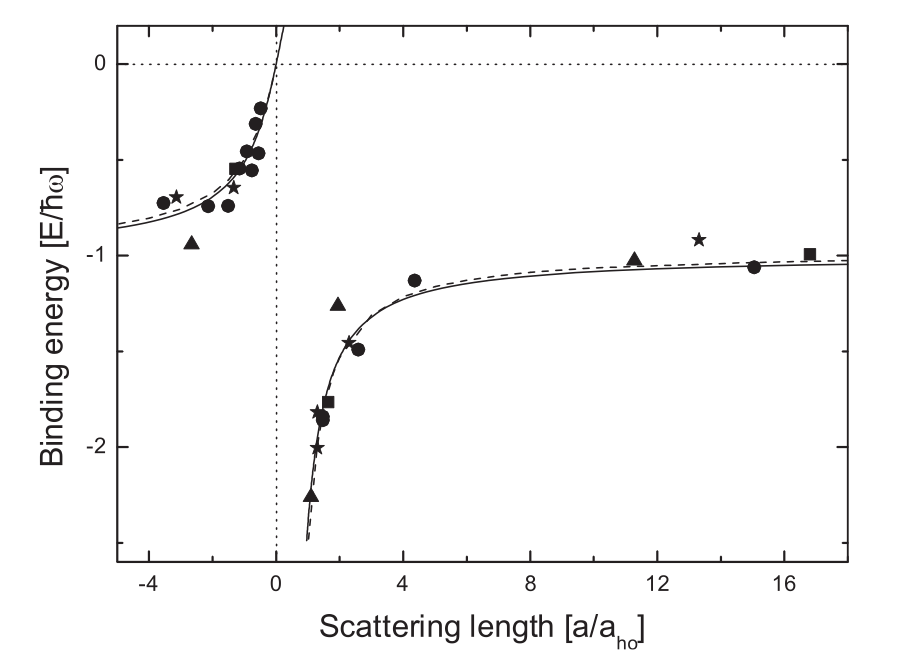
\includegraphics[width=0.5\textwidth]{chap13dmol.png}
    \bicaption{三维光晶格中的Feshbach分子态。散点代表不同晶格深度的实验数据。实线代表理论数据。摘自 \citep{Esslinger3DMol}}{The measured binding energy of molecules in a 3D optical lattice. Scatterd points for defferent depth of latice. The solid line for theory. Reprinted from \citep{Esslinger3DMol}}
    \label{3dmol}
\end{figure}
实验观测到了较深光晶格内调节磁场形成的Feshbach分子态。
%%%%%%%%%%%%%%%%%%%%%%%%%%%%%%%%%%%%%%%%%%%%%%%%%%%%%%%%%%%%%%%%%%%%%%%%%%
\end{comment}

Serwane F及合作者首先发明了一种可以确定性制备不同原子数目的手段\cite{SerwaneDeterministic},这一思路启发了后续精确制备少体体系并探测量子关联的研究\cite{zurn2012fermionization,WenzFermiSeaOnebyOne,Zurn2013Pairing,MurmannSpinChain,MurmannTwoFermionDoubleWell,RontaniTunneling}。研究者利用能级间距较大的微观束缚阱(mircotrap)与两分量${}^6$Li原子热库接触到热平衡,制备$T/T_F\sim0.08$含有600多个原子的费米球。然后在微观束缚阱内施加磁场梯度,使得阱内一端势能降低,然后绝热地改变微观束缚阱的深度,便可使得原子不断漏出,最终制备了只含有几个原子的少体实际物理体系。如图~\ref{deter}~所示。
%%%%%%%%%%%%%%%%%%%%%%%%%%%%%%%%%%%%%%%%%%%%%%%%%%%%%%%%%%%%%%%%%%%%%%%%%%
\begin{figure}[!htbp]
    \centering
    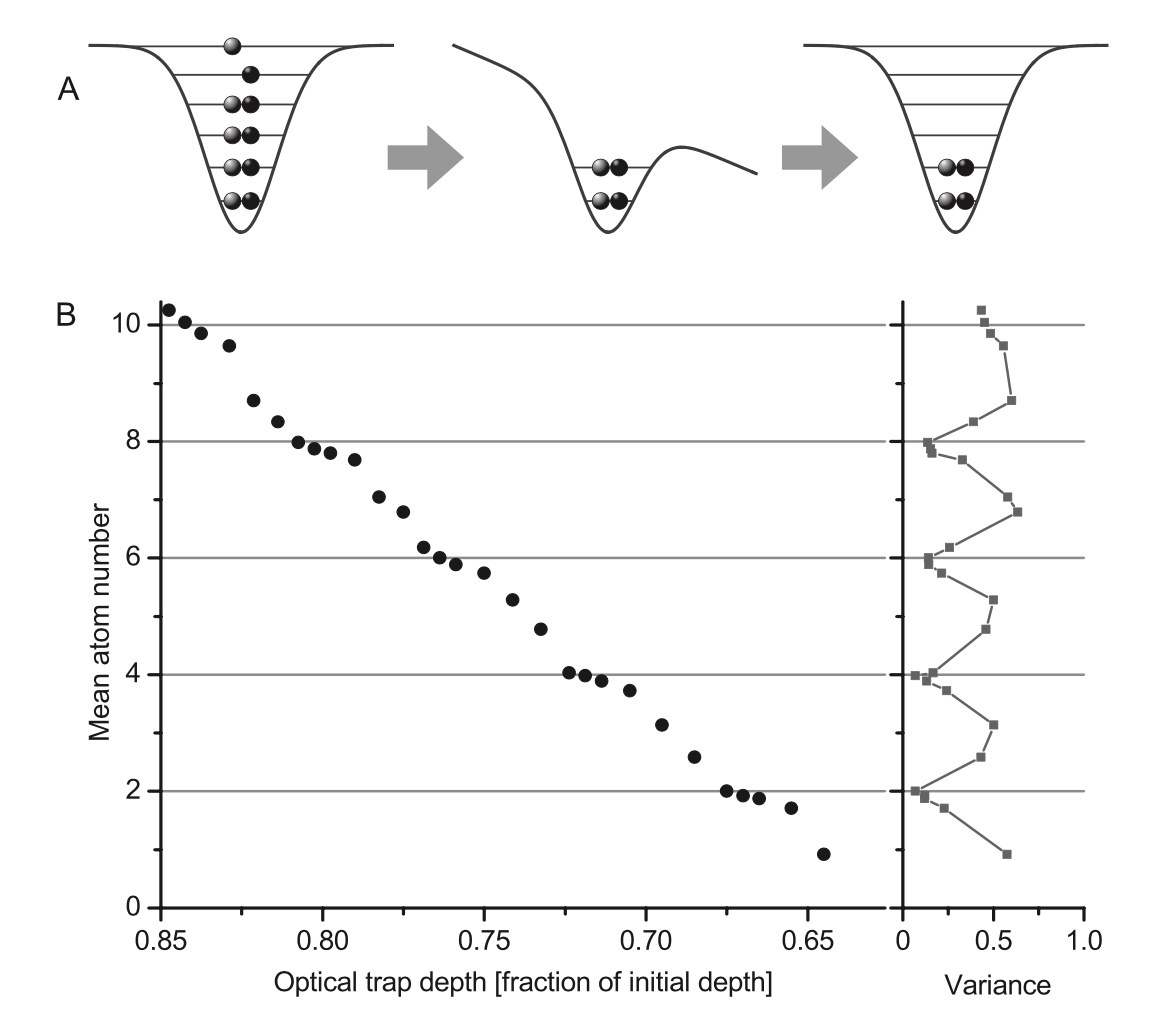
\includegraphics[width=0.5\textwidth]{./intro/chap1deter.png}
    \bicaption{图A表示降低一侧势阱深度使原子漏出来制备少体体系的示意图。图B为实验测到的少体体系平均粒子数与方差。 摘自 \citep{SerwaneDeterministic} }{Fig A for illustration of spilling. Fig B for measured mean density and variance. Reprinted from\citep{SerwaneDeterministic} }
    \label{deter}
\end{figure}
%%%%%%%%%%%%%%%%%%%%%%%%%%%%%%%%%%%%%%%%%%%%%%%%%%%%%%%%%%%%%%%%%%%%%%%%%%

借助上面精确制备少体体系的方法,研究者研究了不同自旋费米子($\uparrow\downarrow$)之间在强相互作用下发生费米化的过程\cite{zurn2012fermionization}。在准一维束缚阱中制备两体少体体系,调节不同自旋费米子之间的相互作用,通过少体体系隧穿几率反映两体体系的能量。最终得到隧穿几率如图~\ref{ferminization}~
%%%%%%%%%%%%%%%%%%%%%%%%%%%%%%%%%%%%%%%%%%%%%%%%%%%%%%%%%%%%%%%%%%%%%%%%%%
\begin{figure}[!htbp]
    \centering
    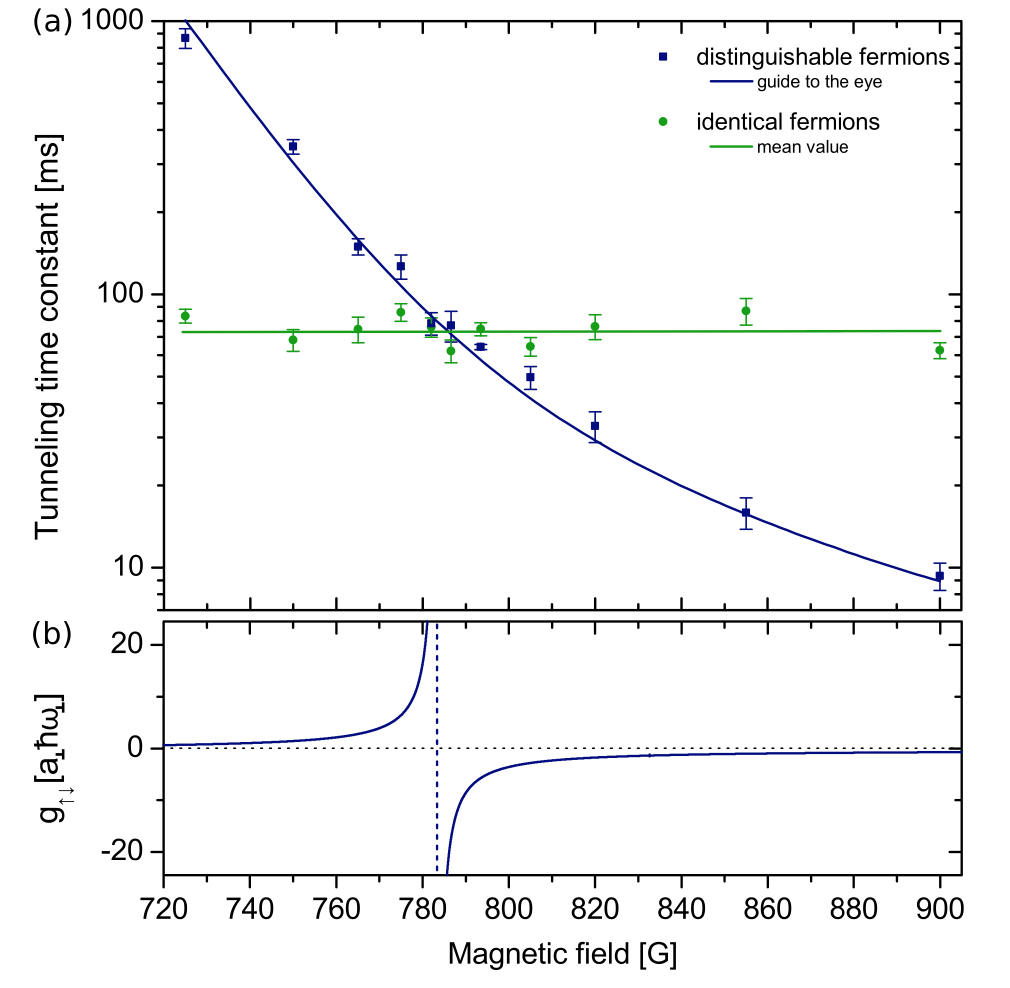
\includegraphics[width=0.5\textwidth]{./intro/chap1ferminization.png}
    \bicaption{不同的有效一维相互作用下两体费米子隧穿几率。谐振子势阱中两体体系的能量决定了隧穿几率。其中在共振点处相互作用费米子$\uparrow\downarrow$能量等于无相互作用全同费米子$\uparrow\uparrow$能量,发生费米化。 摘自 \citep{zurn2012fermionization} }{Tunneling time constant for different 1D effective interaction strengths. Two body energy decides the tunneling time constant. The same tunneling constant of $\uparrow\downarrow$ at resonance point as $\uparrow\uparrow$ reflects the ferminization. Reprinted from\citep{zurn2012fermionization} }
    \label{ferminization}
\end{figure}
%%%%%%%%%%%%%%%%%%%%%%%%%%%%%%%%%%%%%%%%%%%%%%%%%%%%%%%%%%%%%%%%%%%%%%%%%%
所示,同自旋费米子之间无相互作用,调节磁场后两体能级没有变化。但是不同费米子之间相互作用导致散射长度在共振点处发散,对应能量与无相互作用费米子能量相同,体系发生费米化。

进一步地,基于类似的少体制备方法,实验研究者逐步增加粒子数,研究从少体到多体的过渡\cite{WenzFermiSeaOnebyOne}。相关的基本模型为谐振子势阱下N+1的一维极化子物理。相互作用只存在于少数原子与多数原子之间,并且可以通过Feshbach共振调节。从1到5增加多数原子的数目,用射频脉冲测量不同相互作用下极化子的能量,通过与理论计算的1+1与1+$\infty$体系的能量密度进行比较,可以发现在粒子数为5的时候能量密度就很接近多体体系了。如图~\ref{fermisea}~所示。
%%%%%%%%%%%%%%%%%%%%%%%%%%%%%%%%%%%%%%%%%%%%%%%%%%%%%%%%%%%%%%%%%%%%%%%%%%
\begin{figure}[!htbp]
    \centering
    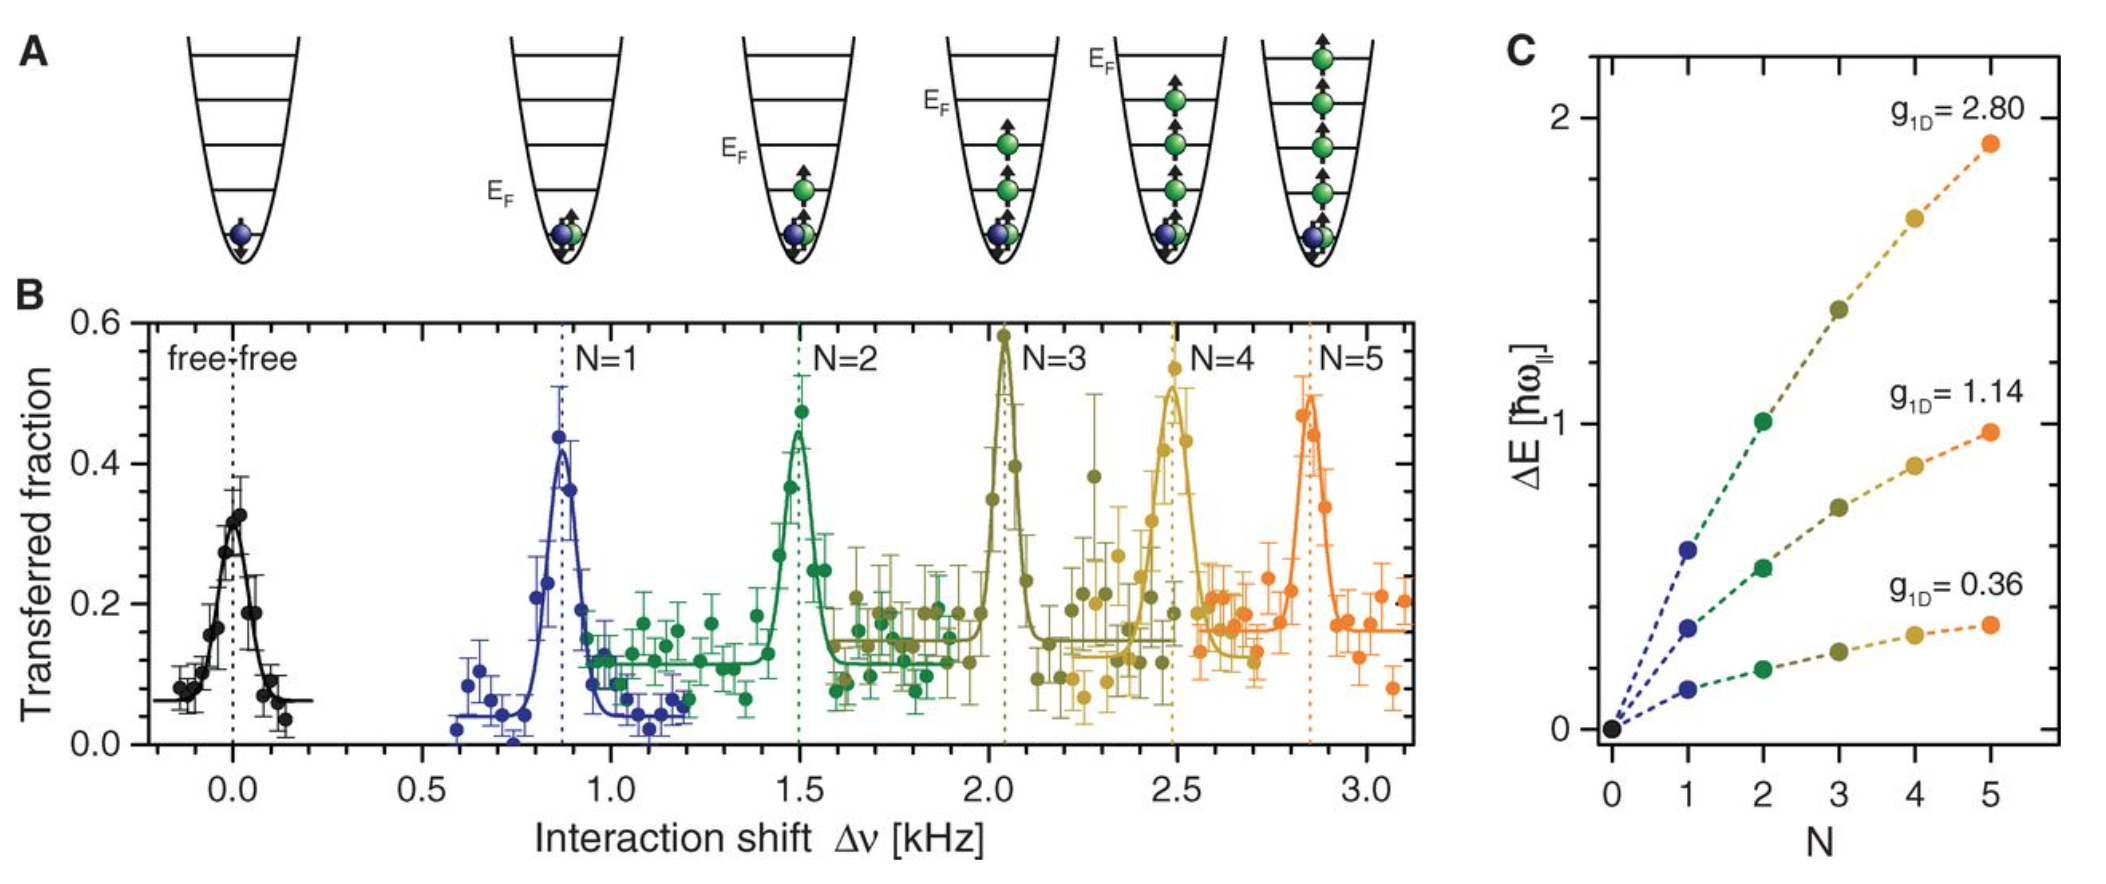
\includegraphics[width=0.8\textwidth]{./intro/chap1fermisea.png}
    \bicaption{ 图A为谐振子势阱中1+N体系能谱示意图。图B为实验测得的射频脉冲谱。图C为能量密度。摘自 \citep{WenzFermiSeaOnebyOne} }{Fig A for energy spectrum of 1+N system. Fig B for measured rf spectrum. Fig C for energy difference. Reprinted from\citep{WenzFermiSeaOnebyOne} }
    \label{fermisea}
\end{figure}
%%%%%%%%%%%%%%%%%%%%%%%%%%%%%%%%%%%%%%%%%%%%%%%%%%%%%%%%%%%%%%%%%%%%%%%%%%

少体物理之所以重要是因为能够在理论方面提供一个可理解的物理图像,在某些特殊极限下甚至存在严格解。这些少体图像构成了我们理解物理的基石。在冷原子领域,有两个经典的两体图像,分别是:自由空间s波散射图像与谐振子势场下s波接触相互作用两体能谱图像。其中前者用来有效地描述相互作用,后者来理解相互作用较强时候系统的能谱与波函数。

1998年, Busch T给出了一个两体体系严格解\cite{busch1998two}:任意维度下两个全同玻色子在谐振子势场下的能谱。虽然是玻色子体系,但是这个严格解同样适用于可分辨费米子。三维情况下,可分辨两体全同费米子位于谐振子外势下,系统的哈密顿量可以写为:
\begin{equation}
\hat{H}=-\frac{1}{2} \nabla_{1}^{2}-\frac{1}{2} \nabla_{2}^{2}+\frac{1}{2} r_{1}^{2}+\frac{1}{2} r_{2}^{2}+4 \pi a_{0} \delta^{(3)}_{reg}\left(\Vector{r}_{1}-\Vector{r}_{2}\right)
\end{equation}
能量量纲为$\hbar\omega$,长度量纲为$\sqrt{\hbar}{m\omega}$,$a_0$代表散射长度。其中$m$为粒子质量,$\omega$为谐振子势场的特征频率,$\delta_{reg}^{(3)}(\Vector{r}) \equiv \delta^{(3)}(\Vector{r})(\partial / \partial r) r$。分离质心运动$\Vector{R}=\sqrt{1 / 2}\left(\Vector{r}_{1}+\Vector{r}_{2}\right)$与相对运动$\Vector{r}=\sqrt{1 / 2}\left(\Vector{r}_{1}-\Vector{r}_{2}\right)$
得到:
\begin{equation}
\begin{aligned}
&\hat{H}_{\mathrm{CM}}=-\frac{1}{2} \nabla_{R}^{2}+\frac{1}{2} \Vector{R}^{2}\\
&\hat{H}_{rel}=-\frac{1}{2} \nabla_{r}^{2}+\frac{1}{2} \Vector{r}^{2}+\sqrt{2} \pi a_{0} \delta^{(3)}(\Vector{r}) \frac{\partial}{\partial r} r\\
\end{aligned}
\end{equation}
质心运动的部分是自由谐振子,剩余相对运动部分满足的薛定谔方程为:
\begin{equation}
\left(\hat{H}_{o s c}+\sqrt{2} \pi a_{0} \delta^{(3)}(\Vector{r}) \frac{\partial}{\partial r} r\right) \Psi(\Vector{r})=E \Psi(\Vector{r})
\end{equation}
相对运动部分的$l\neq0$空间不受相互作用影响,仍为自由谐振子,只考虑$l=0$子空间。波函数展开在谐振子基矢下:
相应的本征波函数为:
\begin{equation}
\Psi(\Vector{r})=\sum_{n=0}^{\infty} c_{n} \varphi_{n}(\Vector{r})
\end{equation}
带入到薛定谔方程里得到:
\begin{equation}
c_{n}\left(E_{n}-E\right)+\sqrt{2} \pi a_{0} \varphi_{n}^{*}(0)\left[\frac{\partial}{\partial r}\left(r \sum_{m=0}^{\infty} c_{m} \varphi_{m}(\Vector{r})\right)\right]_{r \rightarrow 0}=0
\end{equation}
求得$c_n$满足:
\begin{equation}
c_{n}=A \frac{\varphi_{n}^{*}(0)}{E_{n}-E}
\end{equation}
将系数带回到薛定谔方程得到本征能量满足:
\begin{equation}
\sqrt{2} \frac{\Gamma(-E / 2+3 / 4)}{\Gamma(-E / 2+1 / 4)}=\frac{1}{a_{0}}
\end{equation}
对应的本征波函数解析形式为:
\begin{equation}
\Psi(\Vector{r})=\frac{1}{2} \pi^{-3} / 2 A e^{-r^{2} / 2} \Gamma(-v) U\left(-v, \frac{3}{2}, r^{2}\right)
\end{equation}
其能谱随着散射长度变化如图~\ref{chap1busch}~所示:
%%%%%%%%%%%%%%%%%%%%%%%%%%%%%%%%%%%%%%%%%%%%%%%%%%%%%%%%%%%%%%%%%%%%%%%%%%
\begin{figure}[!htbp]
    \centering
    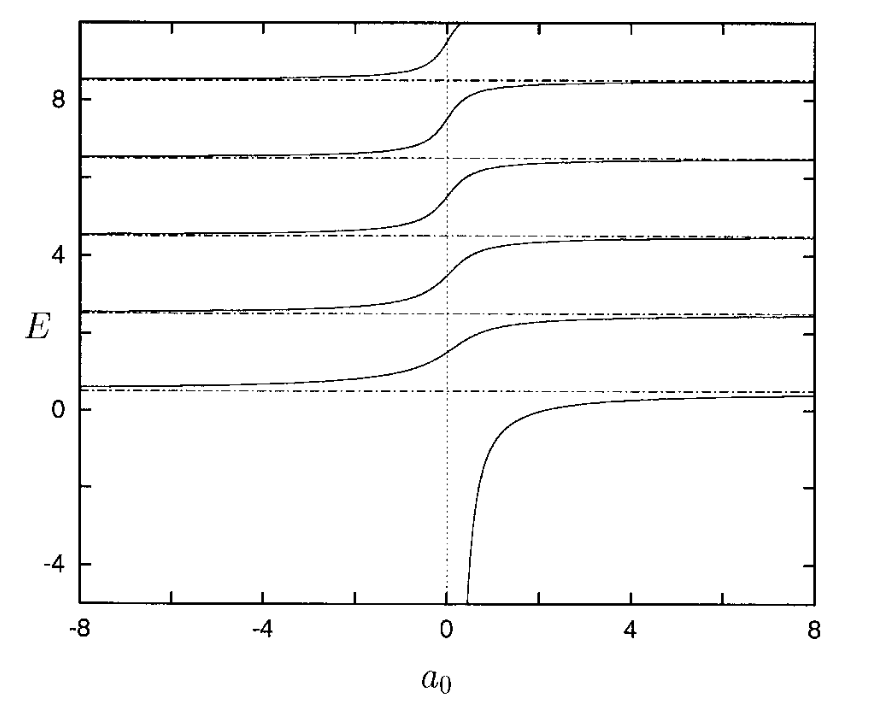
\includegraphics[width=0.6\textwidth]{./intro/chap1busch.png}
    \bicaption{三维下$l=0$空间的两体能谱。摘自\citep{busch1998two} }{Two body spectrum in 3D. Reprinted from \citep{busch1998two} }
    \label{chap1busch}
\end{figure}
%%%%%%%%%%%%%%%%%%%%%%%%%%%%%%%%%%%%%%%%%%%%%%%%%%%%%%%%%%%%%%%%%%%%%%%%%%
当$a_0\to \infty$时候,基态能量渐近行为是$E_g\propto - 1/a_0^2$,称为吸引低能支(attractive lower branch);其余的随着$a_0\to\infty$本征能量饱和在奇数谐振子能量的态称为排斥高能支(repulsive upper branch)。这个少体体系的严格解在后续的实验与理论发展中起了很重要的作用。

类似地,一维以及二维的结果也可用上述求解过程给出。其中一维的能量方程与三维相同,不同在于仅满足偶宇称的解受到相互作用影响。二维下能量方程则有很大不同:
\begin{equation}
\psi(-E / 2+1 / 2)=\log \left(\frac{1}{2 a_{0}^{2}}\right)
\end{equation}

后续对这个体系的严格解有了一些扩展,主要是各向异性的谐振子外势求解,以及动力学研究,更多详细内容请参见\cite{blume2012few}。

如果再增加一个粒子,这个三体体系则没有解析解,只能通过数值手段去求解。我们以$\uparrow\downarrow\uparrow$的费米子三体体系为例,仅在不同自旋费米子之间有s波散射相互作用\cite{OlshaniiRigorous2001,Petrov2003unitary3b,Fleix2006prlunitary3b,Felix2006praunitary3b,LmDuan2007levelcrossing,Stetcu2007,Blume2008,Blume2010,Xiaji2009prl,Xiaji20103b,Rittenhouse2010green}。我们用Bethe-Peierls条件代替相互作用:
\begin{equation}
\psi\left(\Vector{r}_{1}, \Vector{r}_{2}, \Vector{r}_{3}\right)=\left(\frac{1}{r_{i j}}-\frac{1}{a}\right) A\left(\Vector{R}_{i j}, \Vector{r}_{k}\right)+O\left(r_{i j}\right)
\end{equation}
其中$r_{i j} \equiv\left|\Vector{r}_{i}-\Vector{r}_{j}\right| \rightarrow 0$,$\Vector{R}_{ij}$为两原子的质心位置。

\begin{comment}
三维情况下这种体系的求解\cite{Fleix2006prlunitary3b}借助于超球(Hypersphere)框架,先引入Jacobi坐标:
\begin{equation}
\begin{split}
\Vector{r}&=\Vector{r}_{2}-\Vector{r}_{1}\\
\boldsymbol{\rho}&=\left(2 \Vector{r}_{3}-\Vector{r}_{1}-\Vector{r}_{2}\right) / \sqrt{3}\\
\Vector{C}&=\left(\Vector{r}_{1}+\Vector{r}_{2}+\Vector{r}_{3}\right) / 3\\
\end{split}
\end{equation}
然后定义超半径(hyperradius)与超角度(hyperangle):
\begin{equation}
\begin{split}
R&=\sqrt{\left(r^{2}+\rho^{2}\right) / 2}\\
\alpha&=\arctan (r / \rho)\\
\end{split}
\end{equation}
这时候谐振子外势只出现在$R$的薛定谔方程中。考虑波函数形式:
\begin{equation}
\psi\left(\Vector{r}_{1}, \Vector{r}_{2}, \Vector{r}_{3}\right)=\psi_{\mathrm{c} . \mathrm{m} .}(\Vector{C}) F(R)(1+\hat{Q}) \frac{1}{r \rho} \varphi(\alpha) Y_{l}^{m}(\boldsymbol{\rho} / \rho)
\end{equation}
其中$Y_l^m$为角动量为$l$的球谐函数。$l$为三体内部相对角动量。$\hat{Q}=-\hat{P}_{13}$将上式带入薛定谔方程得到$\alpha$满足:
\begin{equation}
\begin{gathered}
-\varphi^{\prime \prime}(\alpha)+\frac{l(l+1)}{\cos ^{2} \alpha} \varphi(\alpha)=s^{2} \varphi(\alpha) \\
\varphi(\pi / 2)=0 \\
\varphi^{\prime}(0)+\eta(-1)^{l} \frac{4}{\sqrt{3}} \varphi(\pi / 3)=0
\end{gathered}
\end{equation}
其中$\eta=-1$。对任意$l$,可以解得一系列$s_{l,n},n=0,1,2,3...$均为实数。如图~\ref{Sv}~
\begin{figure}[!htbp]
    \centering
    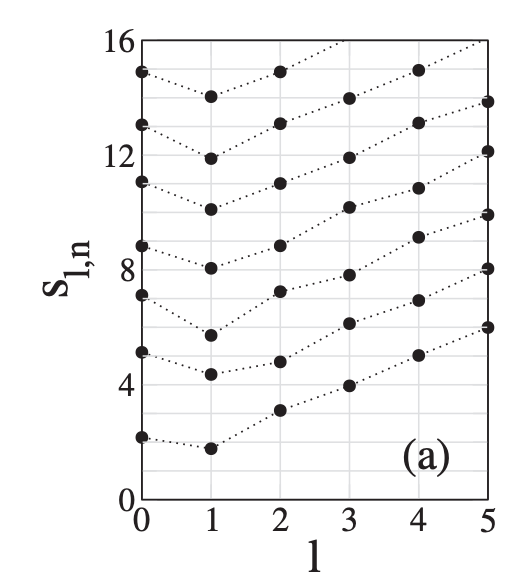
\includegraphics[width=0.5\textwidth]{chap13fSv.png}
    \bicaption{幺正极限下$\uparrow\downarrow\uparrow$三体体系$s_{l,n}$数值结果。摘自\citep{Fleix2006prlunitary3b} }{Numerical $s_{l,n}$ of $\uparrow\downarrow\uparrow$ three fermion system under unitary limit. Reprinted from \citep{Fleix2006prlunitary3b}}
    \label{Sv}
\end{figure}
将解到的$s_{l,n}$带入:
\begin{equation}
\left[-\frac{\hbar^{2}}{2 m}\left(\frac{d^{2}}{d R^{2}}+\frac{1}{R} \frac{d}{d R}\right)+U(R)\right] F(R)=\left(E-E_{\mathrm{c} . \mathrm{m} .}\right) F(R)
\end{equation}
其中$U(R)=\hbar^{2} s^{2} /\left(2 m R^{2}\right)+m \omega^{2} R^{2} / 2$。即可求得三体本征解。

基于上述框架,当s波相互作用处于幺正极限$a\to+\infty$时候,我们可以得到解析解,本征波函数为:
\begin{equation}
 F(R)=R^{s} e^{-R^{2} / 2 a_{\mathrm{ho}}^{2}} L_{q}^{(s)}\left(R^{2} / a_{\mathrm{ho}}^{2}\right)
\end{equation}
其中$a_{ho}=\sqrt{\hbar/m\omega}$,$s$为其中一个$s_{l,n}$,$L^{(\cdot)}_q$为q阶广义拉盖尔多项式,$q$为任意非负整数。能谱为:
\begin{equation}
E=E_{\mathrm{c} . \mathrm{m} .}+\left(s_{l, n}+1+2 q\right) \hbar \omega
\end{equation}

对于非幺正极限的相互作用情况,只能完全借助数值方法。Duan\cite{LmDuan2007levelcrossing}用格林函数的方法数值求解了整个相互作用区间。与上述框架稍有不同,哈密顿量为:
\begin{equation}
\begin{aligned}
&{\left[-\frac{\hbar^{2}}{m_{0}}\left(\nabla_{\Vector{x}}^{2}+\nabla_{\Vector{y}}^{2}\right)+\frac{1}{4} m_{0} \omega^{2}\left(\Vector{x}^{2}+\Vector{y}^{2}\right)-E\right] \Psi(\Vector{x}, \Vector{y})} \\
&\quad=-\sum V\left(\Vector{r}_{\pm}\right) \Psi(\Vector{x}, \Vector{y})
\end{aligned}
\end{equation}
其中$\Vector{y}$为两个$\uparrow$费米子间相对位置。$\frac{\sqrt{\Vector{x}}}{2}$为$\downarrow$费米子相对两$\uparrow$费米子质心的相对位置。波函数在氢原子本征基矢下下展开,求解格林函数并利用边界条件,其中$\Vector{r}_{\pm}=\sqrt{3} \Vector{x} / 2 \pm \Vector{y} / 2$。
\begin{equation}
\begin{aligned}
&\Psi(\Vector{x}, \Vector{y})= \int d \Vector{x}^{\prime} d \Vector{y}^{\prime} G_{E}^{(2)}\left(\Vector{x}, \Vector{y} ; \Vector{x}^{\prime}, \Vector{y}^{\prime}\right)\times \sum_{\pm} \frac{\mp \hbar^{2} f\left(\Vector{r}^{\prime}{ }_{\perp, \pm}\right)}{m_{0}} \delta\left(\Vector{r}^{\prime}{ }_{\pm}\right)\\
&G_{E}^{(2)}\left(\Vector{x}, \Vector{y} ; \Vector{x}^{\prime}, \Vector{y}^{\prime}\right)=\sum_{\lambda_{1} \lambda_{2}} \frac{\psi_{\lambda_{1}}(\Vector{x}) \psi_{\lambda_{2}}(\Vector{y}) \psi_{\lambda_{1}}^{*}\left(\Vector{x}^{\prime}\right) \psi_{\lambda_{2}}^{*}\left(\Vector{y}^{\prime}\right)}{E_{\lambda_{1}}+E_{\lambda_{2}}-E}\\
\end{aligned}
\end{equation}
其中$\psi_\lambda(\Vector{r}) = R_{nl}(r)Y_l^m(\theta,\phi)$,$\lambda = (n,l,m),n=0,1,2...,l=0,1,2...$,$\Vector{r}_{\perp, \pm}=\Vector{x} / 2 \mp \sqrt{3} \Vector{y} / 2$边界条件为:
\begin{equation}
\Psi(\Vector{x}, \Vector{y}) \simeq \mp \frac{f\left(\Vector{r}_{\perp, \pm}\right)}{4 \pi \Vector{r}_{\pm}}\left(1-\frac{\Vector{r}_{\pm}}{a}\right) \text { for } \Vector{r}_{\pm} \rightarrow 0
\end{equation}
进一步将$f\left(\Vector{r}_{\perp}\right)$展开:
\begin{equation}
f\left(\Vector{r}_{\perp}\right)=\Sigma_{\lambda} f_{\lambda} \psi_{\lambda}\left(\Vector{r}_{\perp}\right)
\end{equation}
得到$f_\lambda$满足的矩阵方程:
\begin{equation}
\sum_{\lambda^{\prime}} A_{\lambda^{\prime}} f_{\lambda^{\prime}}=\left[\frac{d}{a}-2 \frac{\Gamma\left(\frac{3 / 2+E_{\lambda} / \hbar \omega-E / \hbar \omega}{2}\right)}{\Gamma\left(\frac{1 / 2+E_{\lambda} / \hbar \omega-E / \hbar \omega}{2}\right)}\right] f_{\lambda},
\end{equation}
其中:
\begin{equation}
A_{\lambda \lambda^{\prime}}=\int \frac{d \Vector{r}_{\perp}}{4 \pi d^{3} \hbar \omega} G_{E-E_{\lambda^{\prime}}}\left(\frac{\sqrt{3} \Vector{r}_{\perp}}{2}, 0\right) \psi_{\lambda}^{*}\left(\Vector{r}_{\perp}\right) \psi_{\lambda^{\prime}}\left(\frac{-\Vector{r}_{\perp}}{2}\right)
\end{equation}
最终得到能谱如图~\ref{duancrossing}~所示,通过跟两体能量的比较作者进一步发现了能级交叉。
\begin{figure}[!htbp]
    \centering
    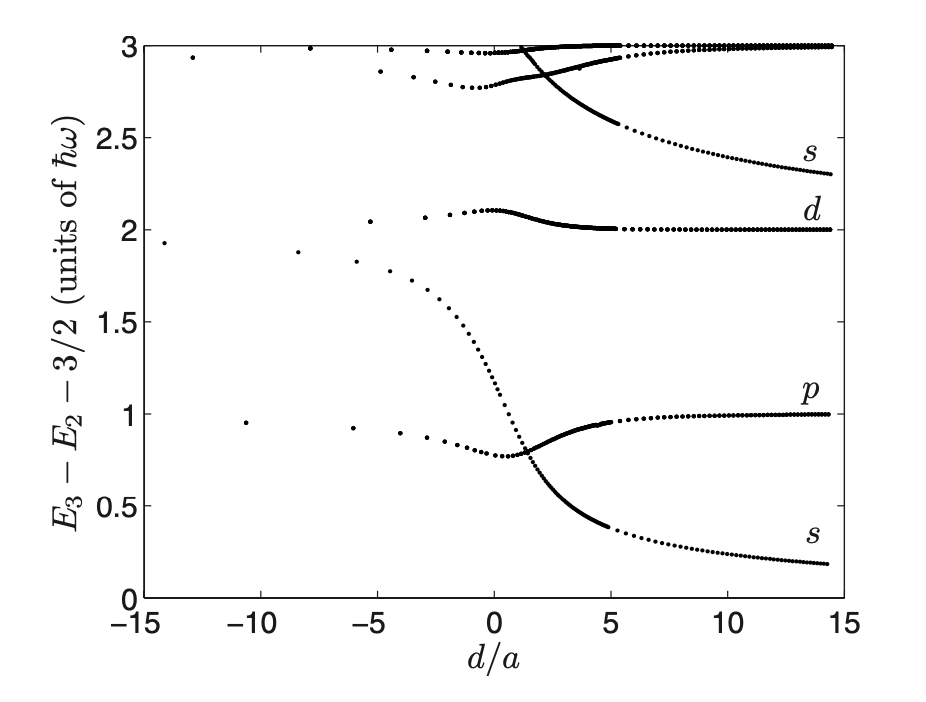
\includegraphics[width=0.7\textwidth]{chap1duan.png}
    \bicaption{三维下三费米子体系($\uparrow\downarrow\uparrow$)能谱。摘自\citep{LmDuan2007levelcrossing}}{Spectrum
     of three fermions system($\uparrow\downarrow\uparrow$)in 3D. Reprinted from \citep{LmDuan2007levelcrossing}}
    \label{duancrossing}
\end{figure}
\end{comment}

三体体系的求解用到两体本征波函数作为基矢\cite{Xiaji2009prl},三体波函数为:
\begin{equation}
\begin{split}
\psi_{3 b}^{\mathrm{rel}}(\Vector{r}, \rho)&=\left(1-\mathcal{P}_{13}\right) \chi(\Vector{r}, \rho)\\
\chi(\Vector{r}, \rho)&=\sum a_{n} \psi_{2 b}^{\mathrm{rel}}\left(r ; v_{l, n}\right) R_{n l}(\rho) Y_{l}^{m}(\hat{\rho})\\
\end{split}
\end{equation}
其中$\psi_{2 b}^{\mathrm{rel}}$代表费米子1,2相对运动的波函数,对应能量为$E_{2b}=(2v_{l,n}+3/2)\hbar\omega$,而$R_{nl}(\rho Y^m_l(\hat{\rho}))$,其中$l,m$是系统的好量子数,代表了相对角动量与其沿z方向的分量。其物理图像非常清晰,将其中一个$\uparrow$费米子与$\downarrow$费米子结合在一起成为二聚体,第三个费米子相对于这个二聚体的运动由$a_n$所描述。最终求解方程:
\begin{equation}
\begin{split}
&\frac{2 \Gamma\left(-v_{l, n}\right)}{\Gamma\left(-v_{l, n}-1 / 2\right)} a_{n}+\frac{(-1)^{l}}{\sqrt{\pi}} \sum_{n^{\prime}} C_{n n^{\prime}} a_{n^{\prime}}=\left(\frac{d}{a}\right) a_{n}\\
&C_{n n^{\prime}} \equiv \int_{0}^{\infty} \rho^{2} d \rho R_{n l}(\rho) R_{n^{\prime} l}\left(\frac{\rho}{2}\right) \psi_{2 b}^{\mathrm{rel}}\left(\frac{\sqrt{3} \rho}{2} ; v_{l, n^{\prime}}\right)\\
\end{split}
\end{equation}
其能谱如图~\ref{xiaji3d}~所示。
%%%%%%%%%%%%%%%%%%%%%%%%%%%%%%%%%%%%%%%%%%%%%%%%%%%%%%%%%%%%%%%%%%%%%%%%%%
\begin{figure}[!htbp]
    \centering
    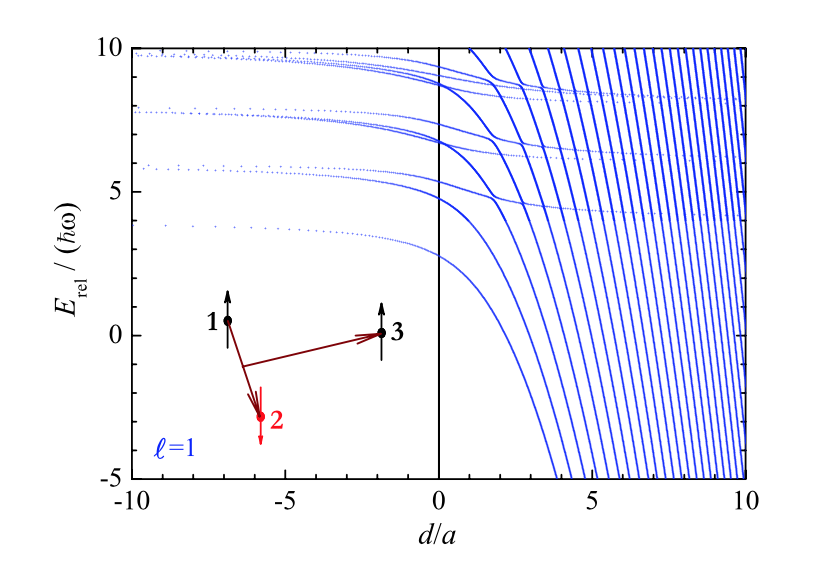
\includegraphics[width=0.6\textwidth]{./intro/chap1xiaji.png}
    \bicaption{三维下三费米子体系($\uparrow \downarrow \uparrow$)的能谱。摘自\citep{Xiaji2009prl}}{Spectrum of three fermions system($\uparrow\downarrow\uparrow$) in 3D. Reprinted from \citep{Xiaji2009prl}}
    \label{xiaji3d}
\end{figure}
%%%%%%%%%%%%%%%%%%%%%%%%%%%%%%%%%%%%%%%%%%%%%%%%%%%%%%%%%%%%%%%%%%%%%%%%%%
后续研究者\cite{Xiaji20103b}还研究了二维体系下三体精确解,采用类似的基矢展开,
\begin{equation}
\begin{split}
\psi_{3 f}^{r e l}&=\left(1-\mathcal{P}_{13}\right) \chi(\Vector{r}, \vec{\rho})\\
\chi(\Vector{r}, \vec{\rho})&=\sum_{n} a_{n}^{f} \psi_{2 p}^{r e l}\left(\Vector{r} ; \nu_{m, n}\right) R_{n m}(\rho) \frac{e^{i m \varphi}}{\sqrt{2 \pi}}\\
\end{split}
\end{equation}
得到整个相互作用区间的的能谱。同时研究者研究了从三维到二维一维的渡越\cite{blume2012},通过各向异性的谐振子束缚体系的求解来研究维度的渡越。而在严格一维体系里面,三费米子的严格求解则由\cite{Rittenhouse2010green,d2014three,loft2015variational,andersen2016interpolatory,bellotti2017comparing}给出。
采用的波函数为:
\begin{equation}
\begin{split}
\psi_{3 F}(x, y)&=\left(1-\boldsymbol{P}_{13}\right) \Omega(x, y)\\
\Omega(x, y)&=\sum_{n=0}^{\infty} a_{n} \psi_{n}^{2b}(x) R_{n}(y)\\
\psi_{n}^{2b}(x)&=\Gamma\left(-v_{n}\right) \mathrm{e}^{-\frac{x^{2}}{2}} U\left(-v_{n}, \frac{1}{2}, x^{2}\right)\\
\end{split}
\end{equation}
其中$\psi_{n}^{2b}(x)$为两体相互作用在谐振势中的解,$R_{n}(y)$为谐振子的本征解。类似地,带入到Bethe–Peierls边界条件中得到耦合方程:
\begin{equation}
\begin{aligned}
&2 g \sum_{n} a_{n}\left[\sqrt{\pi} \frac{\Gamma\left(-v_{n}\right)}{\Gamma\left(-v_{n}+1 / 2\right)} R_{n}(y)-\psi_{n}\left(\frac{\sqrt{3}}{2} y\right) R_{n}\left(-\frac{y}{2}\right)\right] \\
&=-4 \sqrt{\pi} \sum_{n} a_{n} R_{n}(y)
\end{aligned}
\end{equation}
其能谱结构与三维下三体能谱类似。

\begin{comment}
相应地能谱如图~\ref{1d3b}~所示。
%%%%%%%%%%%%%%%%%%%%%%%%%%%%%%%%%%%%%%%%%%%%%%%%%%%%%%%%%%%%%%%%%%%%%%%%%%
\begin{figure}[!htbp]
    \centering
    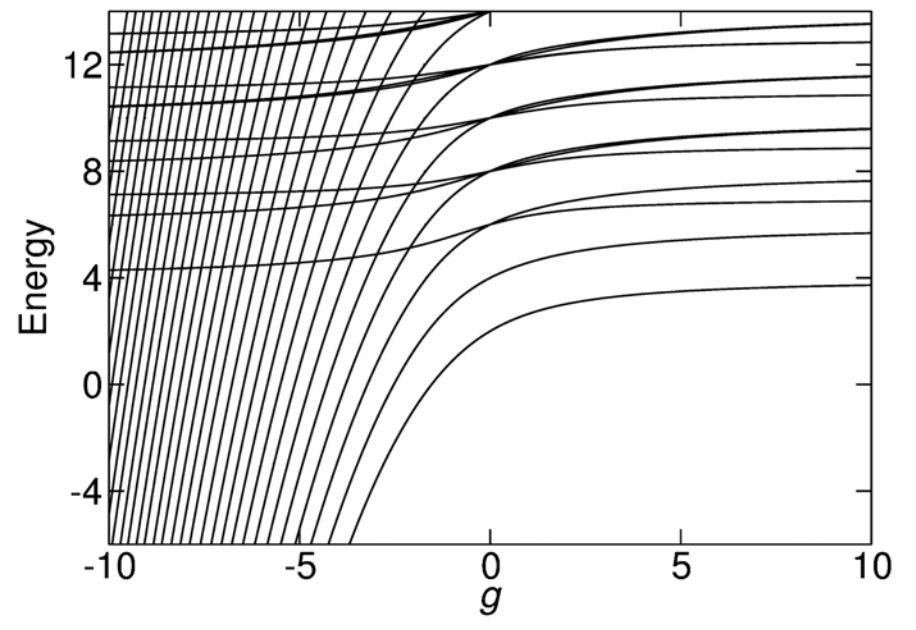
\includegraphics[width=0.7\textwidth]{chap11d3b.png}
    \bicaption{一维下三费米子体系$\uparrow \downarrow \uparrow$的能谱。摘自\citep{d2014three} }{Spectrum of three fermion system($\uparrow\downarrow\uparrow$ in 1D. Reprinted from \citep{d2014three}}
    \label{1d3b}
\end{figure}
%%%%%%%%%%%%%%%%%%%%%%%%%%%%%%%%%%%%%%%%%%%%%%%%%%%%%%%%%%%%%%%%%%%%%%%%%%
\end{comment}

继续增加粒子的数目到四体甚至五体,有一些数值结果\cite{Blume2010,blume2012few},不过如何有效地求解这类体系依然是一个开放问题。多粒子体系中唯一的例外就是在严格一维时候,可以利用贝特假设严格求解,通常情况下贝特假设结果的物理意义不容易提取,但是在某些极限下却有清楚的物理图像,这其中一个典型例子就是Tonks极限及其附近的自旋链模型\cite{Guan2009exact,ma2009mathematical,Lewenstein2013spinchain,volosniev2014strongly,Busch013spinchain,CuiHo2014,Santos2014spinchain,Puhan2015spinchain,Yang2016effective}。
这一模型最早在冷原子少体物理中得以实现,制备$(N_\uparrow,N_\downarrow)=(2,1,(3,1),(2,2)$少体体系,绝热地调节不同自旋之间相互作用从自由极限到Tonks极限,越过共振点进入super Tonks极限,制备了反铁磁自旋链与铁磁自旋链,其中蕴含的少体关联也直接由实验成功探测\citep{MurmannSpinChain}。

\begin{comment}
\begin{figure}[!htbp]
    \centering
    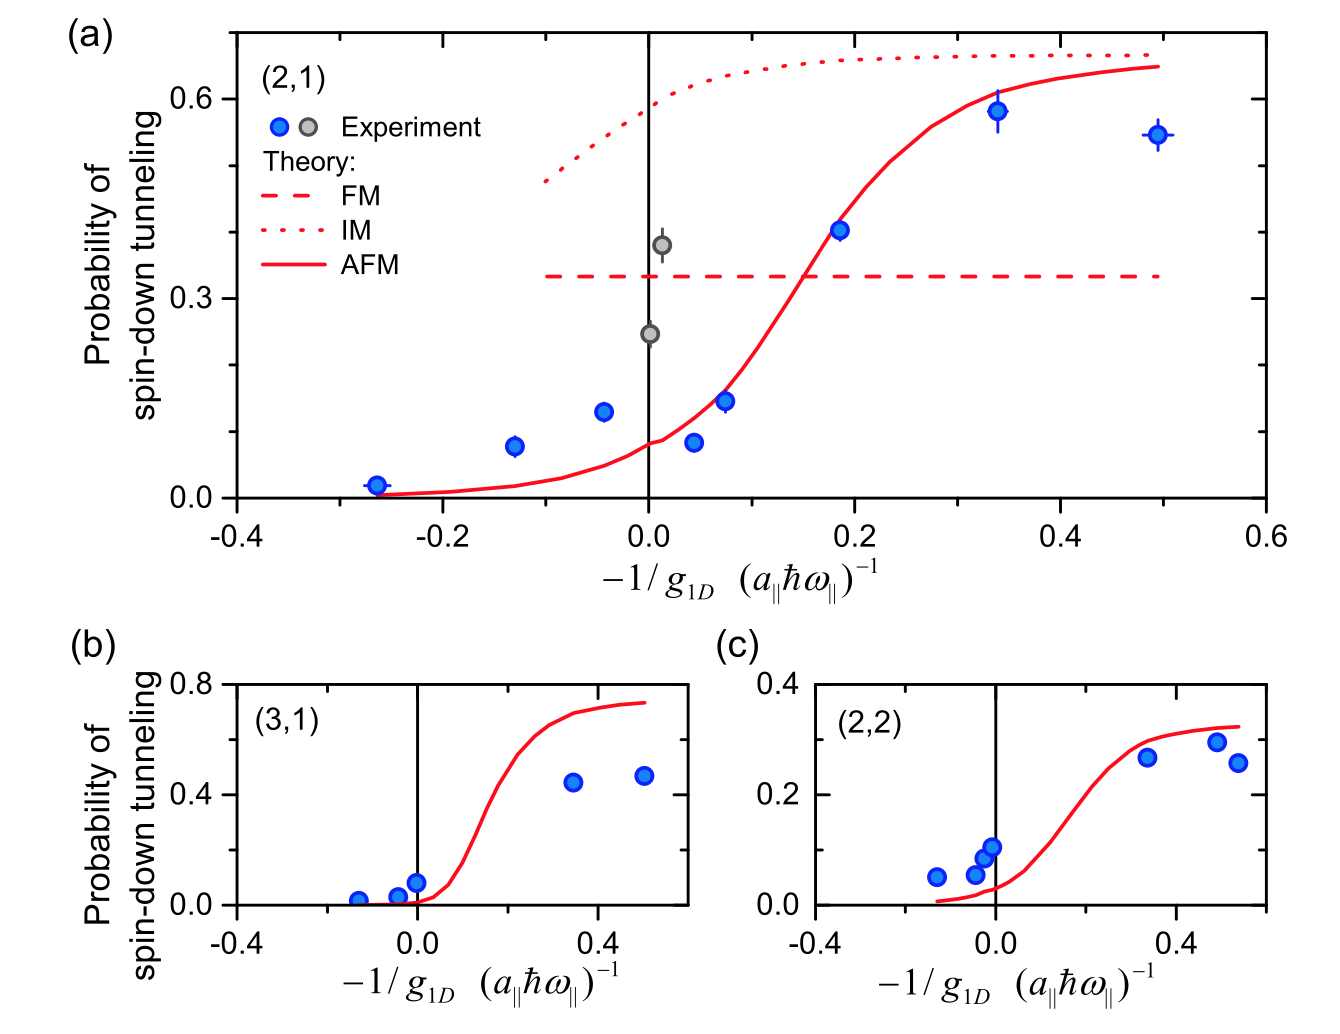
\includegraphics[width=0.7\textwidth]{chap1spinchain.png}
    \bicaption{ 不同少体体系$\downarrow$原子隧穿几率随一维有效相互作用的变化,a为(2,1),b为(3,1),c为(2,2)。散点为实验测得数据。线条代表不同的自旋链模型计算得到的隧穿几率。摘自 \citep{MurmannSpinChain} }{Tunneling rate of $\downarrow$ atom in different few body systems upon 1D effective coupling constant. a for (2,1), b for (3,1) and cc for (2,2). Reprinted from\citep{MurmannSpinChain} }
    \label{chap1spinchainexp}
\end{figure}
%%%%%%%%%%%%%%%%%%%%%%%%%%%%%%%%%%%%%%%%%%%%%%%%%%%%%%%%%%%%%%%%%%%%%%%%%%
实验上通过让边缘处的粒子漏出,来测量自旋分布。漏出的几率由初态能量与末态能量决定。通过与理论自旋链模型的漏出几率对比,可以确认制备到反铁磁自旋链。如图~\ref{chap1spinchainexp}~所示。
\end{comment}

理论方面,对于无限大相互作用的自旋1/2费米子体系的研究则受到Girardeau处理玻色子的启发,研究者求解了带有自旋费米子体系的严格解\cite{Guan2009exact},其中基态简并是一重要特征。定义N个费米子在一维顺序自旋排布$\xi_{1}, \xi_{2}, \ldots, \xi_{N}$态为:
\begin{equation}
\left|\left\{\xi_{1}, \xi_{2}, \ldots, \xi_{N}\right\}\right\rangle \equiv|\vec{\xi}\rangle
\end{equation}
其坐标表示为:
\begin{equation}
\begin{aligned}
&\langle x_{1}, \ldots, x_{N} ; \mu_{1}, \ldots, \mu_{N} \mid \vec{\xi}\rangle \\
&\quad=\sum_{P} \theta\left(x_{P_{1}}, x_{P 2}, \ldots, x_{P_{N}}\right) \prod_{i} \delta_{\xi_{i}, \mu_{P_{i}}}
\end{aligned}
\end{equation}
其中$P$为$(1,2..,N)$的一个置换。并且:
\begin{equation}
\begin{aligned}
\theta\left(x_{P_{1}}, x_{P 2}, \ldots, x_{P_{N}}\right) &=1 & & \text { 如果 } x_{P_{1}}<x_{P 2}<\cdots<x_{P_{N}} \\
&=0 & & \text { 其它 }
\end{aligned}
\end{equation}
由于体系相互作用仅存在于不同自旋费米子之间,因此总的自旋$\Vector{S}_{tot},S_{tot,z}$守恒。N个费米子在共振点处发生费米化,相互作用转变为边界条件:
\begin{equation}
\left.\Psi\left(x_{1}, \sigma_{1} ; \ldots ; x_{N}, \sigma_{N}\right)\right|_{x_{i}=x_{j}, \sigma_{i}=-\sigma_{j}}=0
\end{equation}
如果其中$M$个$\uparrow$,$N-M$个$\downarrow$,本征波函数具有$C_N^M$重简并:
\begin{equation}
\begin{split}
&\Psi_{F}^{\xi}=\phi_{F}\left(x_{1}, x_{2}, \ldots, x_{N}\right)\langle x_{1}, \ldots, x_{N} ; \mu_{1}, \ldots, \mu_{N} \mid \vec{\xi}\rangle\\
&\phi_{F}\left(x_{1}, x_{2}, \ldots, x_{N}\right) =\frac{1}{\sqrt{N !}} D\left(x_{1}, x_{2}, \ldots, x_{N}\right) \\
&\quad\quad =\prod_{i<j}\left(x_{i}-x_{j}\right) F\left(x_{1}, x_{2}, \ldots, x_{N}\right)\\
\end{split}
\end{equation}
其中$\phi_F$由N个不同谐振子能级构成。一旦相互作用不在共振处,这些简并的能级就会打开简并,其打开简并的方式恰好可以被自旋链模型所描述。
\begin{equation}
\hat{H}_{\mathrm{eff}}=\sum_{l} \frac{J_{l}}{g}\left(\Vector{s}_{l} \cdot \Vector{s}_{l+1}-\frac{1}{4}\right)
\end{equation}
其中自旋之间的耦合常数满足:
\begin{equation}
J_{l}=\left.2 N !\left(\frac{1}{m}\right)^{2} \int d \Vector{x}\left|\frac{\partial \phi_{F}}{\partial x_{i j}}\right|_{x_{i j}=0}\right|^{2} \theta\left(\cdots<x_{i}=x_{j}<\cdots\right)
\end{equation}
具体的计算参见\cite{Guan2009exact,Santos2014spinchain,Yang2016effective}
%%%%%%%%%%%%%%%%%%%%%%%%%%%%%%%%%%%%%%%%%%%%%%%%%%%%%%%%%%%%%%%%%%%%%%%%%%
\begin{figure}[!htbp]
    \centering
    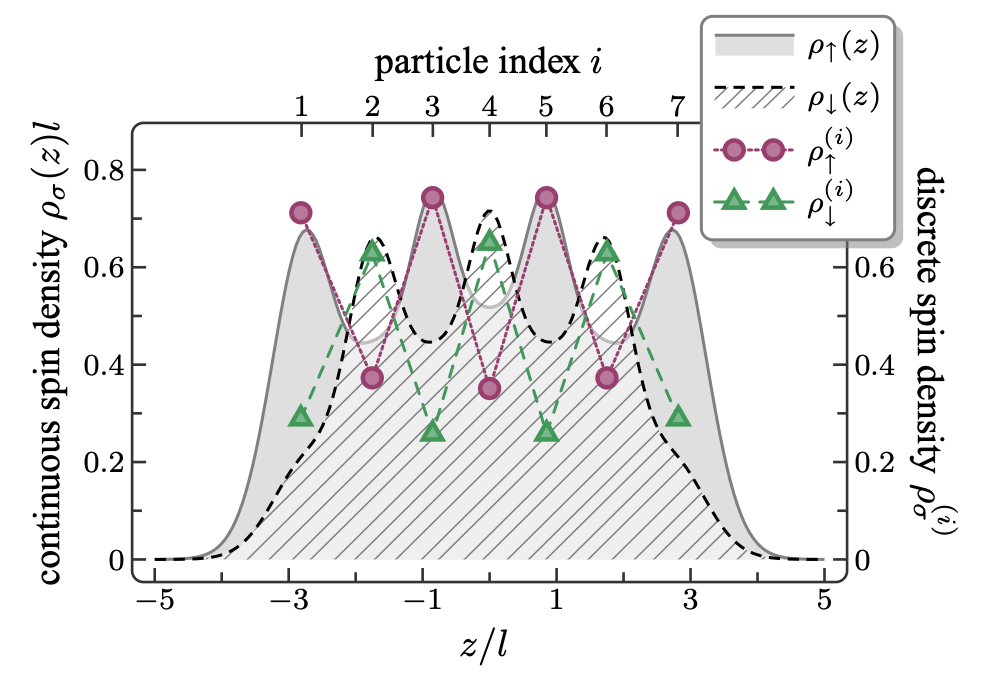
\includegraphics[width=0.6\textwidth]{./intro/chap1spinchainth.png}
    \bicaption{少体自旋1/2费米子体系无限大排斥附近的自旋链有效模型。摘自\citep{Santos2014spinchain} }{Spin-chain representation of an infinitely repulsive system of a few fermions. Reprinted from \citep{Santos2014spinchain}}
    \label{spinchainth}
\end{figure}
%%%%%%%%%%%%%%%%%%%%%%%%%%%%%%%%%%%%%%%%%%%%%%%%%%%%%%%%%%%%%%%%%%%%%%%%%%
\begin{comment}
基于上面介绍的量子少体研究进展,将有几个可扩展的方向,比如改变相互作用,偶极、库伦、以及自旋交换相互作用,这其中自旋交换相互作用将是下一章节要重点介绍的。
\end{comment}











\section{自旋交换相互作用}\label{1sec:spin-exchange}
在超冷原子实验平台中,原子整体作为基本粒子,具有内禀自由度。分为内部电子轨道自由度和核自旋自由度。在冷原子实验平台发展初期,冷却囚禁的原子主要集中在碱金属一族,最外层只有一个电子。后续随着实验技术的进步,碱土金属一族的原子进入到大家的视野。这类原子最外层有两个电子,基态${}^1S_0$与激发态${}^3P_0$都具有较长的寿命,称为轨道自由度。由于不同内部电子结构的原子间相互作用不同,因此不同轨道天然地带来了不同的原子间相互作用。进一步,由于体系温度极低,轨道电子的总角动量$J$为零,碱土金属元素的核自旋自由度可以发挥重大的作用。这就为碱土金属原子作为量子模拟的平台带来丰富的可能性。

最早在碱土金属中做量子模拟的可以追溯到2010年理论想法,基于当时对于费米型碱土金属原子的冷却与调控,Gorshkov A V\cite{gorshkov2010two}及合作者提出了利用这一平台来模拟SU(N)相关的物理。具体地,从两体散射来讲,原子间的相互作用仅与价电子排布有关而与核自旋无关。光晶格中费米型碱土金属原子服从的哈密顿量为:
\begin{equation}
\begin{aligned}
\hat{H}=& \sum_{\alpha m} \int \mathrm{d}^{3} \Vector{r} \hat{\Psi}_{\alpha m}^{\dagger}(\Vector{r})\left(-\frac{\hbar^{2}}{2 M} \nabla^{2}+V_{\alpha,opt}(\Vector{r})\right) \hat{\Psi}_{\alpha m}(\Vector{r}) \\
&+\hbar \omega_{0} \int \mathrm{d}^{3} \Vector{r}\left(\hat{\rho}_{e}(\Vector{r})-\hat{\rho}_{g}(\Vector{r})\right)+ \sum_{\alpha, m<m^{\prime}} g_{\alpha \alpha} \int \mathrm{d}^{3} \Vector{r} \hat{\rho}_{\alpha m}(\Vector{r}) \hat{\rho}_{\alpha m^{\prime}}(\Vector{r})  \\
&+ g_{e g^+} \int \mathrm{d}^{3} \Vector{r} \hat{\rho}_{eg^+}(\Vector{r}) \hat{\rho}_{eg^+}(\Vector{r})+g_{e g^-} \int \mathrm{d}^{3} \Vector{r} \hat{\rho}_{eg^-}(\Vector{r}) \hat{\rho}_{eg^-}(\Vector{r})\\
\end{aligned}
\end{equation}
其中$\alpha=g({^1S_0})$或者$e({}^3P_0)$代表不同电子内态的原子。$m=-I,...,I$对应核自旋分量。$eg^+$与$eg^-$对应散射通道:
\begin{equation}
|eg^{\pm}\rangle = \frac{|ge\rangle\pm|eg\rangle}{\sqrt{2}}\otimes\frac{|\uparrow\downarrow\rangle\mp|\downarrow\uparrow \rangle}{\sqrt{2}}
\end{equation}
因此表征原子间相互作用仅需要四个通道的相互作用常数$g_{gg},g_{ee},g_{eg^+},g_{eg^-}$。
\begin{comment}
如图~\ref{eg}~
%%%%%%%%%%%%%%%%%%%%%%%%%%%%%%%%%%%%%%%%%%%%%%%%%%%%%%%%%%%%%%%%%%%%%%%%%%
\begin{figure}[!htbp]
    \centering
    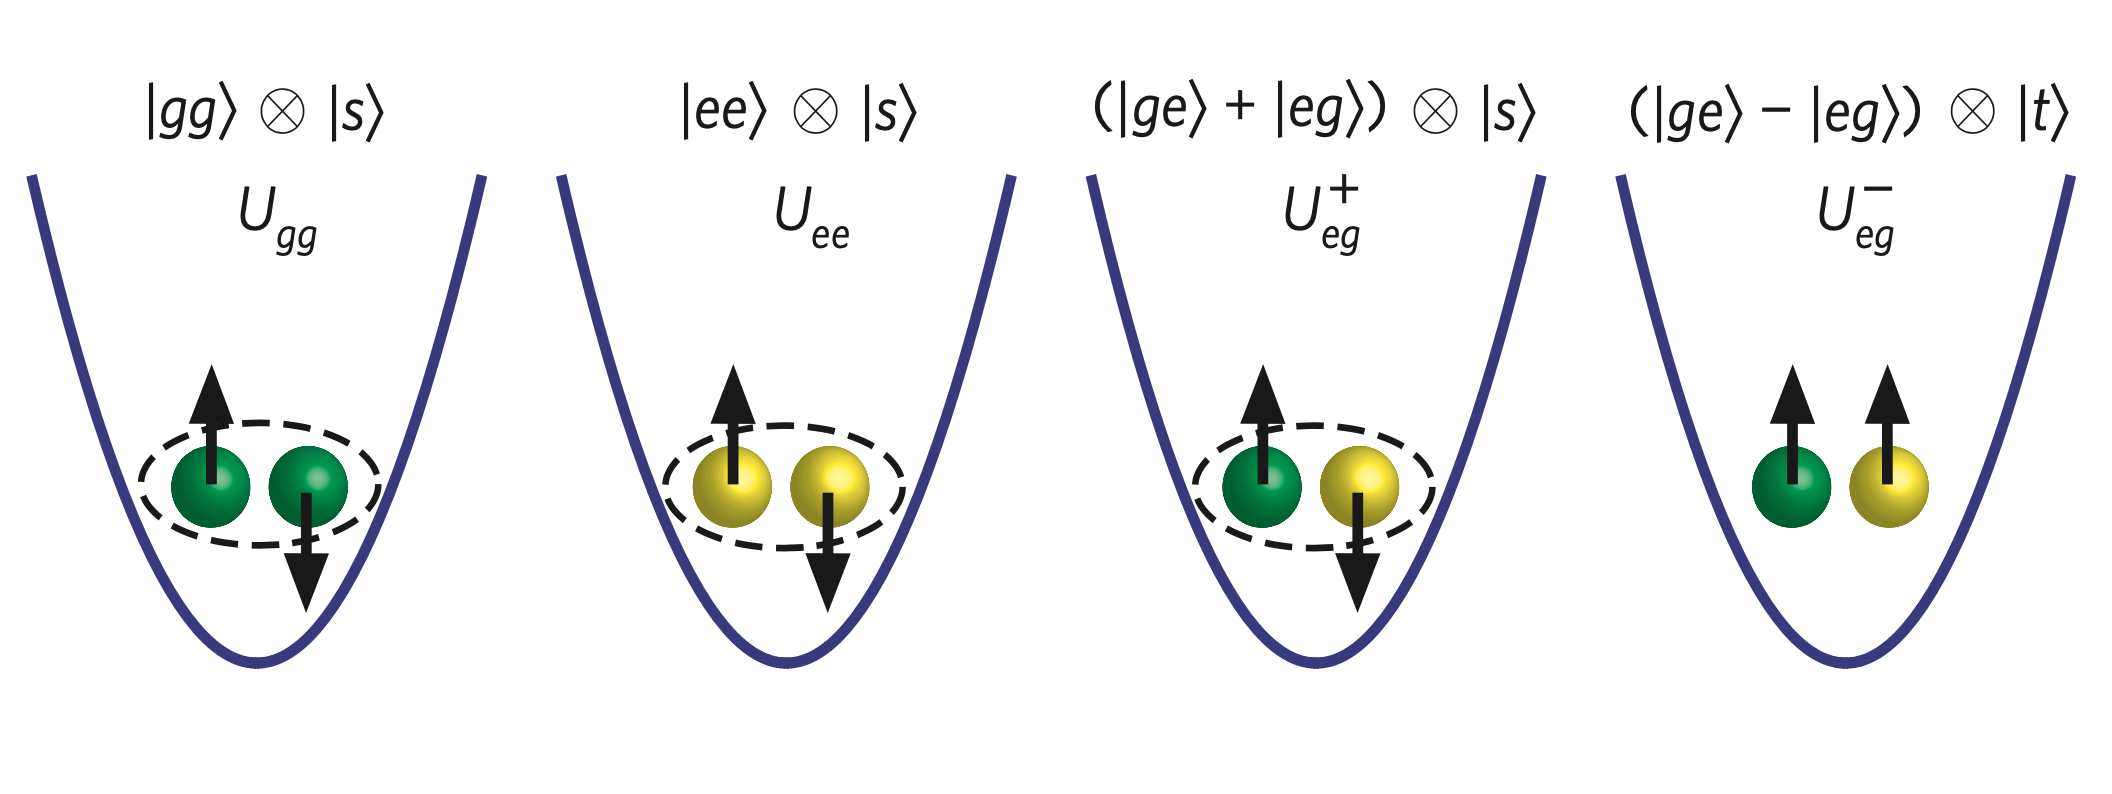
\includegraphics[width=0.7\textwidth]{eg.png}
    \bicaption{光晶格中四个散射通道。摘自\cite{gorshkov2010two}}{Four scattering channels in optical lattice. Reprinted from \cite{gorshkov2010two}}
    \label{eg}
\end{figure}
%%%%%%%%%%%%%%%%%%%%%%%%%%%%%%%%%%%%%%%%%%%%%%%%%%%%%%%%%%%%%%%%%%%%%%%%%%
\end{comment}
如果将$\hat{\rho}_{eg^\pm}$展开,我们得到不同轨道原子间的相互作用$\hat{V}_{eg}$分成了自旋交换与自旋守恒的两项:
\begin{equation}
\begin{aligned}
\hat{V}_{eg^+} &= g_{e g^+} \int \mathrm{d}^{3} \Vector{r} \hat{\rho}_{eg^+}(\Vector{r}) \hat{\rho}_{eg^+}(\Vector{r})+g_{e g^-} \int \mathrm{d}^{3} \Vector{r} \hat{\rho}_{eg^-}(\Vector{r}) \hat{\rho}_{eg^-}(\Vector{r})\\
\quad &= \frac{g_{e g}^{+}+g_{e g}^{-}}{2} \int \mathrm{d}^{3} \Vector{r} \rho_{e}(\Vector{r}) \rho_{g}(\Vector{r}) \\ 
&\quad \quad + \frac{g_{e g}^{+}-g_{e g}^{-}}{2} \sum_{m m^{\prime}} \int \mathrm{d}^{3} \Vector{r} \Psi_{g m}^{\dagger}(\Vector{r}) \Psi_{e m^{\prime}}^{\dagger}(\Vector{r}) \Psi_{g m^{\prime}}(\Vector{r}) \Psi_{e m}(\Vector{r})
\end{aligned}
\end{equation}
最后,将整个二次量子化哈密顿量在光晶格紧束缚近似下写为:
\begin{equation}
\begin{aligned}
\hat{H}=&-\sum_{\langle j, i\rangle \alpha, m} J_{\alpha}\left(c_{i \alpha m}^{\dagger} c_{j \alpha m}+\text { h.c. }\right)+\sum_{j, \alpha} \frac{U_{\alpha \alpha}}{2} n_{j \alpha}\left(n_{j \alpha}-1\right) \\
&+V \sum_{j} n_{j e} n_{j g}+V_{e x} \sum_{j, m, m^{\prime}} c_{j g m}^{\dagger} c_{j e m^{\prime}}^{\dagger} c_{j g m^{\prime}} c_{j e m}
\end{aligned}
\end{equation}
其中$\hat{n}_{j\alpha}=\sum_m \hat{n}_{j\alpha m}$,$V=\left(U_{e g}^{+}+U_{e g}^{-}\right) / 2$与$V_{ex}=\left(U_{e g}^{+}-U_{e g}^{-}\right) / 2$分别描述不同轨道原子间的自旋不变与自旋交换相互作用,其中:
\begin{equation}
U_{eg^\pm} = g_{eg^\pm} \int \mathrm{d}^{3} \Vector{r} w_e^2(\Vector{r})w_g^2(\Vector{r})
\end{equation}
有了上述丰富的轨道间相互作用与核自旋SU(N)自由度,这一模型可以用来模拟众多凝聚态物理中强关联多体模型,比如近藤晶格模型、自旋链模型、自旋液体等。

紧接着于2014年,Scazza F\cite{scazza2014observation}与合作者一起在${}^{173}$Yb体系中证实了上述自旋交换相互作用的存在。其思路如图~\ref{egexp}~所示:
%%%%%%%%%%%%%%%%%%%%%%%%%%%%%%%%%%%%%%%%%%%%%%%%%%%%%%%%%%%%%%%%%%%%%%%%%%
\begin{figure}[!htbp]
    \centering
    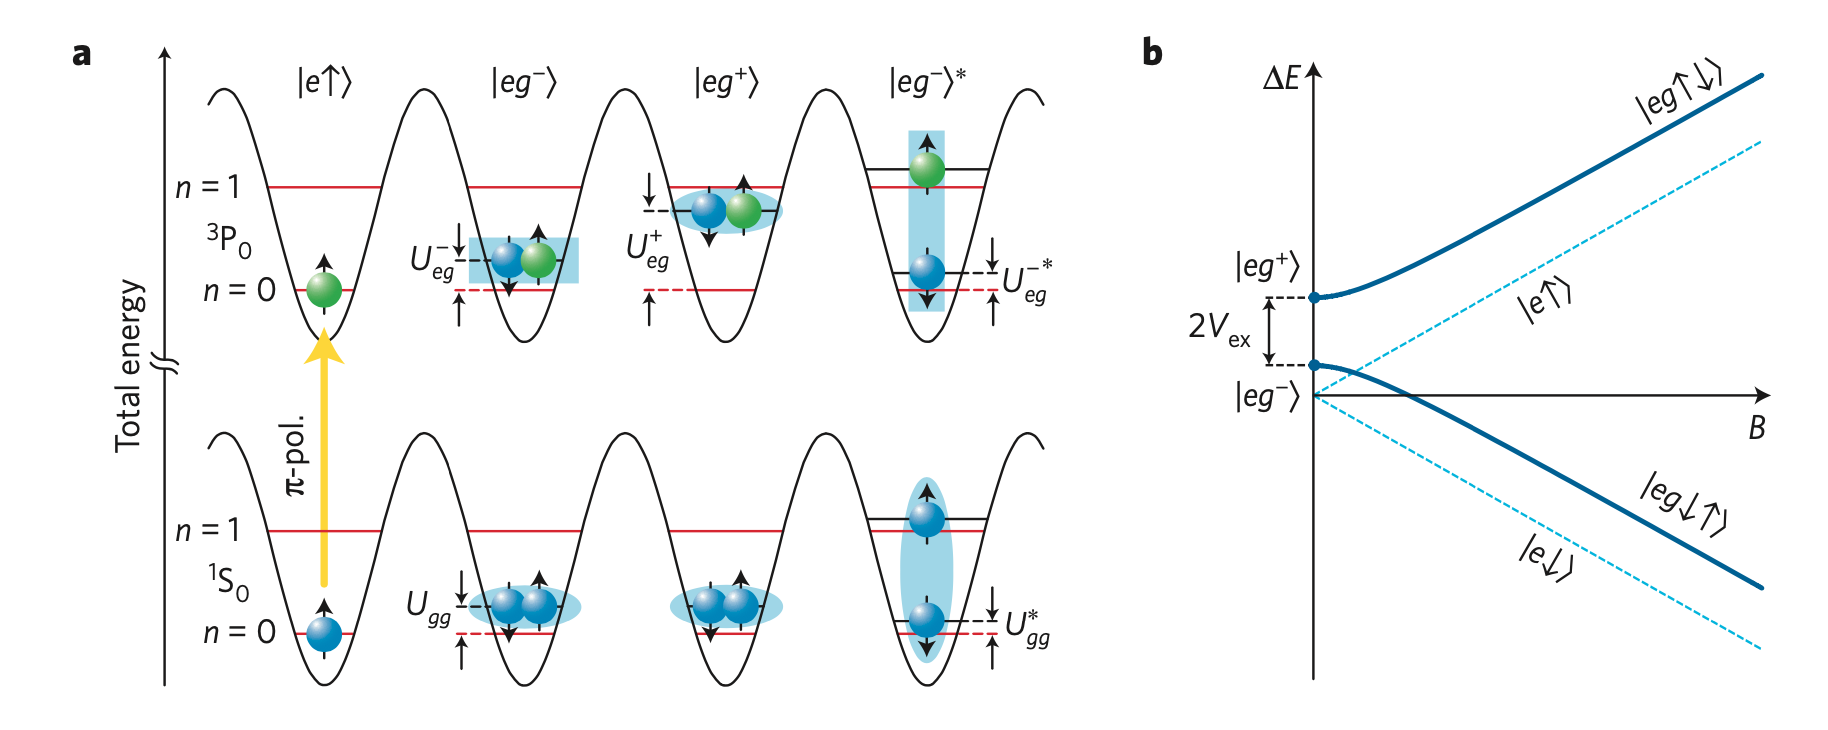
\includegraphics[width=0.7\textwidth]{./intro/egexp.png}
    \bicaption{图a代表单原子与双原子初态到末态的跃迁。图b代表末态的能谱。摘自\citep{scazza2014observation}}{Fig a for transition from initial state to final state under laser field. Fig b for energy spectrum of final state. Reprinted from \citep{scazza2014observation}}
    \label{egexp}
\end{figure}
%%%%%%%%%%%%%%%%%%%%%%%%%%%%%%%%%%%%%%%%%%%%%%%%%%%%%%%%%%%%%%%%%%%%%%%%%%
该实验选取不同电子排布($g({}^1S_0)$与$e({}^3P_0)$)的${}^{173}$Yb($I=5/2$)原子,束缚在较深(原子不能自由移动)的光晶格中,在每个格点里面,原子间的相互作用能为:
\begin{equation}
U_{X}=\frac{4 \pi \hbar^{2}}{m} a_{X} \int \mathrm{d}^{3} r w_{a}^{2}(\Vector{r}) w_{b}^{2}(\Vector{r})
\end{equation}
其中$X =gg, ee, eg^+, eg^−$代表不同状态的原子对。装载不同核自旋的$g$轨道原子到光晶格中,平均填充在$\bar{n}=1$与$\bar{n}=2$之间,这样导致部分格点内有一个原子,部分格点内有两个原子。对于有两个原子的格点,用激光将一个原子从g态激发到e态,末态有两个本征态$|eg^\pm\rangle$,本征能量为$U_{eg^\pm}$。如果在体系中加入沿$z$方向的磁场,导致$|eg^\pm\rangle$两态之间有非零的跃迁矩阵元,最终的哈密顿量为:
\begin{equation}
\hat{H}_{eg}=\left(\begin{array}{cc}
U_{e g}^{+} & \Delta_{B} \\
\Delta_{B} & U_{e g}^{-}
\end{array}\right)
\end{equation}
其中$\Delta_{B}=\delta g m_{\mathrm{F}} \mu_{\mathrm{B}} B$,$\delta g$为核自旋朗德因子的差值,跃迁末态的本征能量为:
\begin{equation}
E_{1,2}=V \pm \sqrt{V_{\mathrm{ex}}^{2}+\Delta_{B}^{2}}
\end{equation}
本征波函数为$|eg^\pm\rangle$两态的线性叠加。

\begin{comment}
如图~\ref{egd}~
%%%%%%%%%%%%%%%%%%%%%%%%%%%%%%%%%%%%%%%%%%%%%%%%%%%%%%%%%%%%%%%%%%%%%%%%%%
\begin{figure}[!htbp]
    \centering
    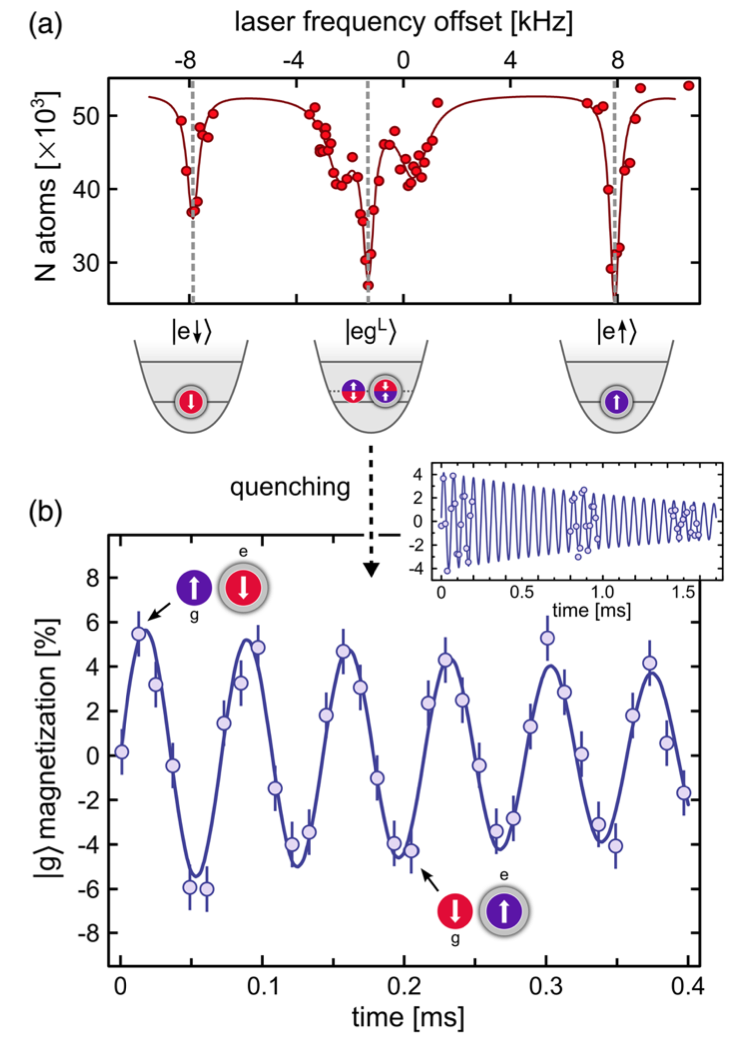
\includegraphics[width=0.6\textwidth]{chap1spexd.png}
    \bicaption{图a代表实验测到的吸收谱,不同的峰代表了不同的末态。图b代表观测到自旋交换体系的的自旋动力学。摘自\citep{cappellini2014direct}}{Fig(A) for spectrum of clock transition. Fig(B) for time resolved spin transition. dynamics. Reprinted from \citep{cappellini2014direct}}
    \label{egd}
\end{figure}
%%%%%%%%%%%%%%%%%%%%%%%%%%%%%%%%%%%%%%%%%%%%%%%%%%%%%%%%%%%%%%%%%%%%%%%%%%
\end{comment}

通过观测不同磁场下的共振谱,得到不同磁场下末态的能量。进一步地,研究者通过测量初态自旋分布到末态自旋分布演化\cite{scazza2014observation,cappellini2014direct},直接观测到了自旋交换相互作用。拟合实验中不同磁场下测到的共振峰的位置,最终测到${}^{173}$Yb原子间裸的散射长度为\cite{scazza2014observation,cappellini2014direct}:
\begin{equation}
\begin{split}
a_{e g}^{-}&=(3300 \pm 300) a_{0}\\
a_{e g}^{+}& = 219.5 a_0\\
\end{split}
\end{equation}
可以看到为铁磁耦合。与此同时,研究者也观测到了Sr原子体系的铁磁自旋交换相互作用\cite{zhang2014spectroscopic}。

但是上述观测到的裸的原子间相互作用为铁磁自旋耦合,模拟近藤物理需要反铁磁耦合。这时候理论研究者提出利用束缚诱导共振来调节,一系列系统的工作表明利用束缚诱导共振来调节反铁磁自旋交换的强度\cite{zhang2016kondo,cheng2017enhancing,zhang2018control,ji2018confinement,zhang2020tight,zhang2020controlling}。最终实验上成功观测到了的准一维体系束缚诱导增强的自旋动力学\cite{riegger2018localized}。如图~\ref{CIRspexexp}~所示。
%%%%%%%%%%%%%%%%%%%%%%%%%%%%%%%%%%%%%%%%%%%%%%%%%%%%%%%%%%%%%%%%%%%%%%%%%%
\begin{figure}[!htbp]
    \centering
    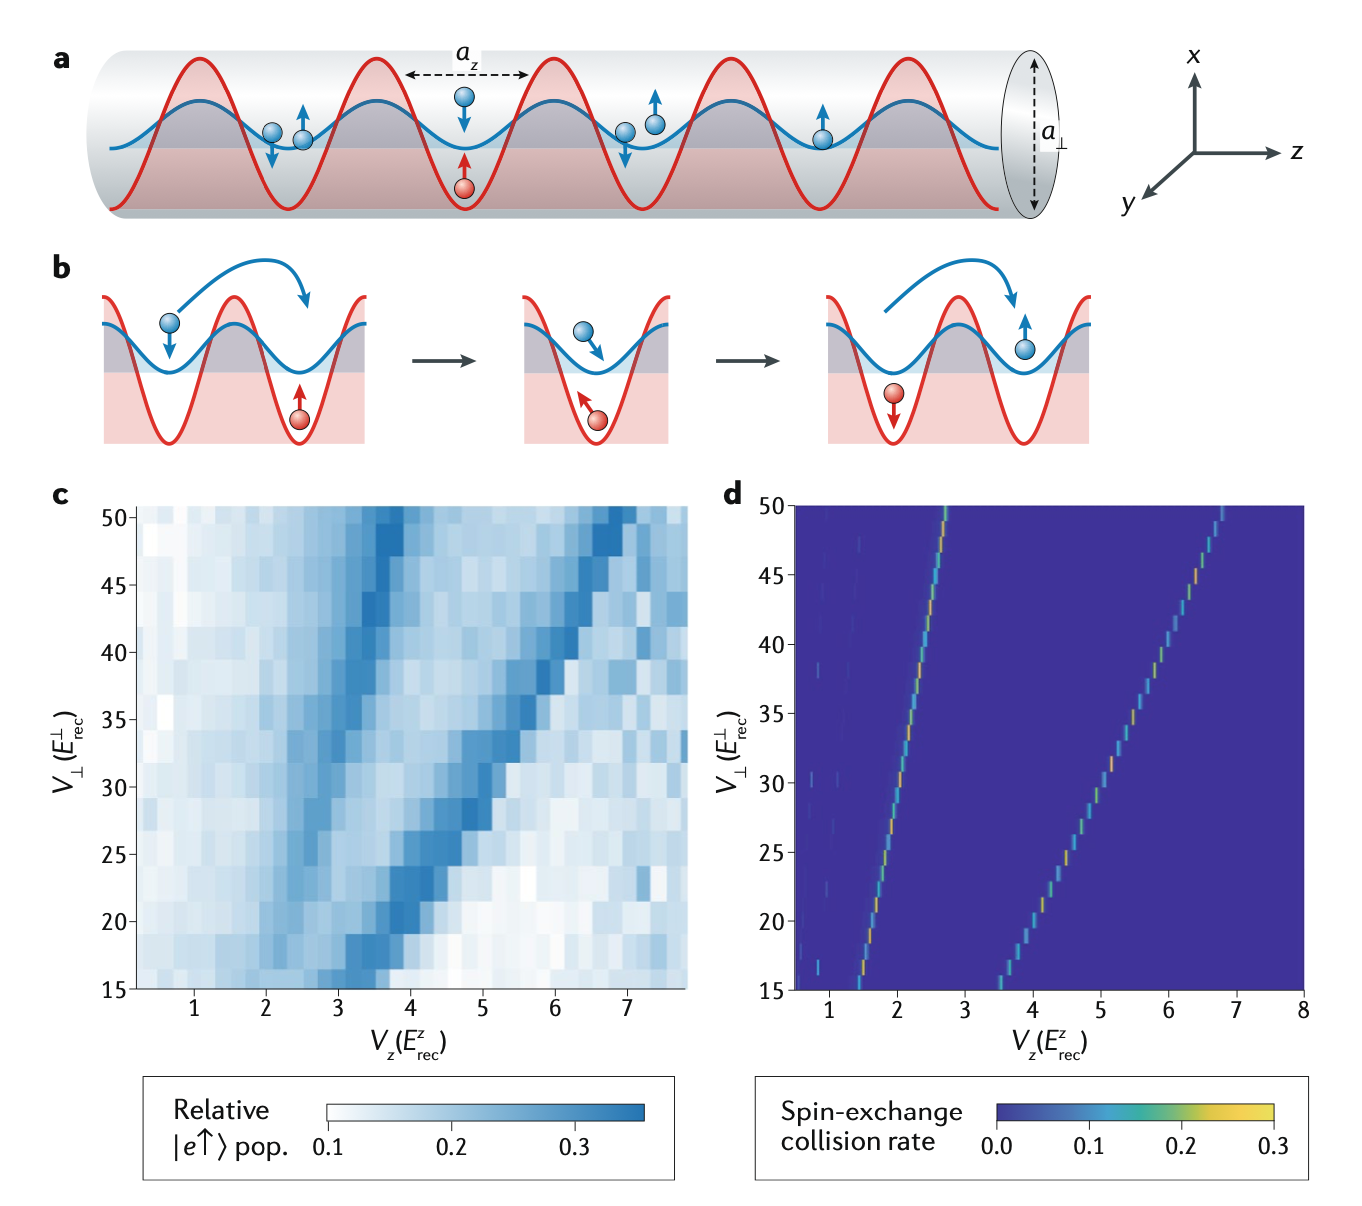
\includegraphics[width=0.7\textwidth]{./intro/chap1spexCIR.png}
    \bicaption{图a代表准一维体系z方向上自旋相关的晶格制造巡游费米子与局域费米子。图b代表自旋交换发生的过程。图c,d分别代表实验测量与理论预测的束缚诱导增强下的自旋交换动力学。摘自\citep{riegger2018localized,zhang2020controlling}}{Fig a for quasi 1D system, which consists of spin-dependent lattice to creat free hopping fermions and localized spin. Fig b for illustration of spin exchange process. Fig c and d for Experimental and theoretical spin exchange interaction enchanced by confinement induced resonance. Reprinted from \citep{riegger2018localized,zhang2020controlling}}
    \label{CIRspexexp}
\end{figure}
%%%%%%%%%%%%%%%%%%%%%%%%%%%%%%%%%%%%%%%%%%%%%%%%%%%%%%%%%%%%%%%%%%%%%%%%%%












\section{费米极化子物理}\label{1sec:polaron}
极化子是一个杂质物理中比较古老的概念。早在固体物理中就有研究大极化子与小极化子\cite{landau1933bewegung,pekar1946autolocalization,frohlich1950xx,frohlich1954electrons,feynman1955slow,mahanmany},对应的是电子在晶格中运动,电子的单粒子性质被晶格声子激发所修饰,改变其有效质量、寿命等。严格说晶格里的极化子属于玻色极化子。如果将背景原子改为多体费米体系,就得到费米极化子。近年来,随着冷原子中密度不均衡费米混合气体的制备,费米极化子作为其中的极端体系,进入研究者的视野,结合冷原子体系特有的控制、操控、观测能力,极化子的研究迎来新的阶段,我们将围绕相关研究的实验与理论展开。

费米极化子是典型的费米液体,冷原子物理中Feshbach可调节相互作用带来了对整个相互作用区间的关注。冷原子中费米极化子的研究最早可追溯到Chevy变分波函数\cite{chevy2006},这是个典型的N+1体系。系统哈密顿量为:
\begin{equation}
\hat{H}=\sum_{k, \sigma} \epsilon_{k} \hat{a}_{k, \sigma}^{\dagger} \hat{a}_{k, \sigma}+\frac{g_{b}}{V_{k, \boldsymbol{k}^{\prime}, q}} \sum_{\boldsymbol{k}+q, 1}^{\dagger} \hat{a}_{\boldsymbol{k}^{\prime}-q, 2}^{\dagger} \hat{a}_{\boldsymbol{k}^{\prime}, 2} \hat{a}_{\boldsymbol{k}, 1}
\end{equation}
采用Chevy变分波函数:
\begin{equation}
\left|\psi_{0}\right\rangle=\left(\phi_{0} d_{\Vector{0}}^{\dagger}+\sum_{\Vector{k}, \Vector{q}}^{\prime} \phi_{\Vector{k q}} d_{\Vector{q}-\Vector{k}}^{\dagger} u_{\Vector{k}}^{\dagger} u_{\Vector{q}}\right)\left|\mathrm{FS}_{\uparrow}^{N}\right\rangle
\end{equation}
带入到薛定谔方程中得到:
\begin{equation}
\begin{split}
&\left(\epsilon_{k}+\epsilon_{q-k}-\epsilon_{q}\right) \phi_{k, q}+\frac{g_{b}}{V} \sum_{k^{\prime}} \phi_{k^{\prime}, q}+\frac{g_{b}}{V} \phi_{0}=E \phi_{k, q}\\
&\frac{g_{b}}{V} \sum_{q} \phi_{0}+\frac{g_{b}}{V} \sum_{q, k} \phi_{k, q}=E \phi_{0}\\
\end{split}
\end{equation}
引入辅助变量$\chi(\boldsymbol{q})=\phi_{0}+\sum_{\boldsymbol{k}} \phi_{k, \boldsymbol{q}}$得到能量满足自洽方程:
\begin{equation}
E=\sum_{q<k_{F}} \frac{1}{\sum_{k>k_{F}}\left(\frac{1}{\epsilon_{\boldsymbol{k}}+\epsilon_{q-k}-\epsilon_{q}-E}-\frac{1}{2 \epsilon_{\boldsymbol{k}}}\right)-\sum_{k<k_{F}} \frac{1}{2 \epsilon_{k}}} \label{consistentEQ}
\end{equation}
%%%%%%%%%%%%%%%%%%%%%%%%%%%%%%%%%%%%%%%%%%%%%%%%%%%%%%%%%%%%%%%%%%%%%%%%%%
\begin{figure}[!htbp]
    \centering
    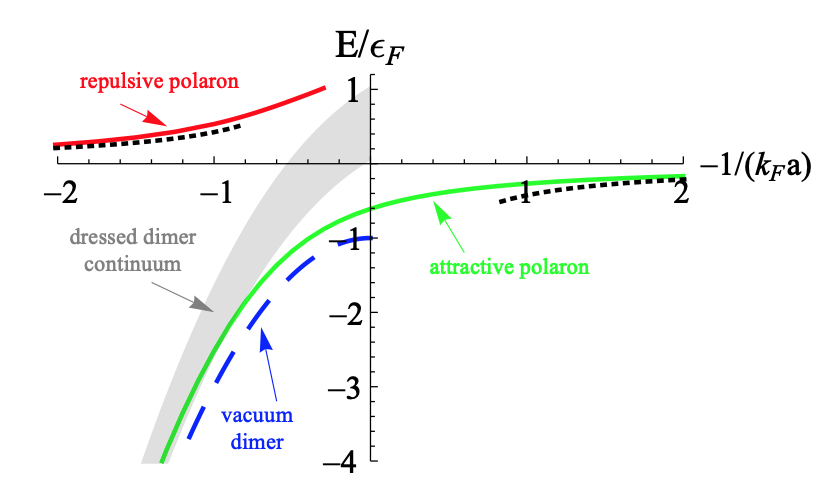
\includegraphics[width=0.7\textwidth]{./intro/chap1fpspectrum.png}
    \bicaption{单粒子空穴近似下的吸引极化子与排斥极化子能量。绿色对应吸引极化子,红色对应排斥极化子的解,中间灰色区域对应分子态。摘自\citep{massignan2014polarons}}{Energy of attractive and repulsive fermi polarons under 1 p-h approximation. Green line for attractive polaron, red line for repulsive polarons and gray area for continuous dreesed molecules.  Reprinted from\citep{massignan2014polarons}}
    \label{fpchevyE}
\end{figure}
%%%%%%%%%%%%%%%%%%%%%%%%%%%%%%%%%%%%%%%%%%%%%%%%%%%%%%%%%%%%%%%%%%%%%%%%%%
求解最低能量可以得到吸引极化子,如图~\ref{fpchevyE}~所示。在弱相互作用区间,基态为极化子态,本征能量为$E_-$,在BCS极限下$E_{-}=2 \pi a n_{\uparrow} / m_{r}$。随着相互作用增强,杂质原子与背景费米海中任意位置的一个原子配对形成分子,带来一段连续能谱区间,宽度大约为$E_F$,其中零动量分子的能量可以利
用新的分子态变分波函数\cite{Mora_pm,Punk_pm,combescot2010analytical,Trefzger2012Impurity}来得到:
\begin{equation}
\left|\psi_{1}\right\rangle=\left(\sum_{\Vector{k}}^{\prime} \xi_{\Vector{k}} d_{-\Vector{k}}^{\dagger} u_{\Vector{k}}^{\dagger}+\sum_{\Vector{k}^{\prime}, \Vector{k}, \Vector{q}}{ }^{\prime} \xi_{\Vector{k}^{\prime} \Vector{k q}} d_{\Vector{q}-\Vector{k}-\Vector{k}^{\prime}}^{\dagger} u_{\Vector{k}^{\prime}}^{\dagger} u_{\Vector{k}}^{\dagger} u_{\Vector{q}}\right)\left|\mathrm{FS}_{\uparrow}^{N-1}\right\rangle
\end{equation}
求得一支被费米海修饰的分子态的能量解,与极化子能量比较可以发现转变点在$1/k_Fa_S=0.84$,如图~\ref{pmE}~所示:
%%%%%%%%%%%%%%%%%%%%%%%%%%%%%%%%%%%%%%%%%%%%%%%%%%%%%%%%%%%%%%%%%%%%%%%%%%
\begin{figure}[!htbp]
    \centering
    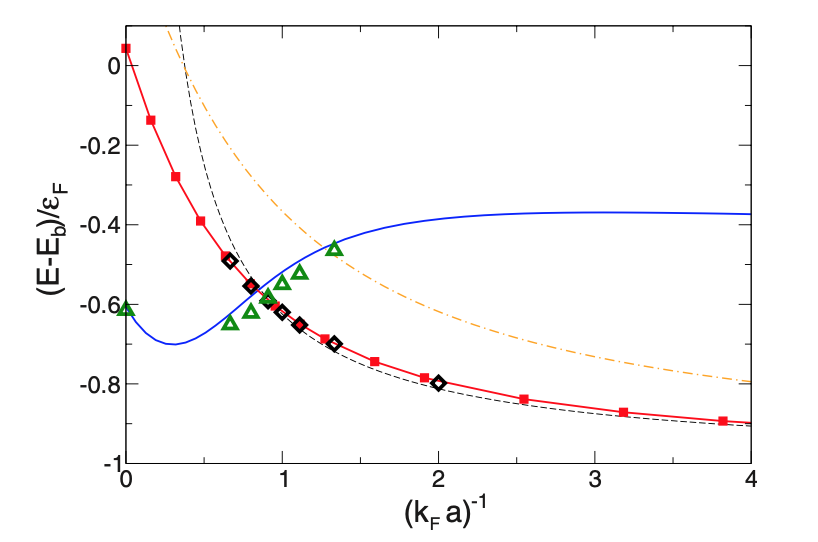
\includegraphics[width=0.7\textwidth]{./intro/chap1pmE.png}
    \bicaption{极化子-分子转变。其中蓝色实线代表一对粒子-空穴激发近似下的零动量极化子。红色实线代表考虑一对粒子空穴激发修饰的分子能量,橘黄色虚线代表费米面存在裸的分子态能量。散点为蒙特卡洛的结果。摘自\citep{Punk_pm}}{Polaron-molecule transition. Blue solid line for zero momentum attractive polaron branch under 1 p-h excitation approximation, red solid line for dreesed molecule under 1 p-h excitation approximation, yellow dashed line for bare molecule with fermi sea. Scatterd points for result from MC. Reprinted from\citep{Punk_pm}}
    \label{pmE}
\end{figure}
%%%%%%%%%%%%%%%%%%%%%%%%%%%%%%%%%%%%%%%%%%%%%%%%%%%%%%%%%%%%%%%%%%%%%%%%%%
极化子到分子的转变除了上述变分方法的研究之外,利用量子蒙特卡罗算法也可以研究极化子体系。最早在极化气体中利用Fixed-node蒙卡算法可以求得低杂质密度下费米液体行为\cite{Pilati2008phase}。 利用图蒙卡可以得到转变点为$1/k_Fa_S=0.9$,相应地极化子与分子的单粒子性质比如有效质量在转变点附近发散,如图~\ref{MCeffectm}~所示。极化子的准粒子剩余等也可以由蒙卡方法得到\cite{Prokoffermi,Prokofbold,VlietinckMC}。
%%%%%%%%%%%%%%%%%%%%%%%%%%%%%%%%%%%%%%%%%%%%%%%%%%%%%%%%%%%%%%%%%%%%%%%%%%
\begin{figure}[!htbp]
    \centering
    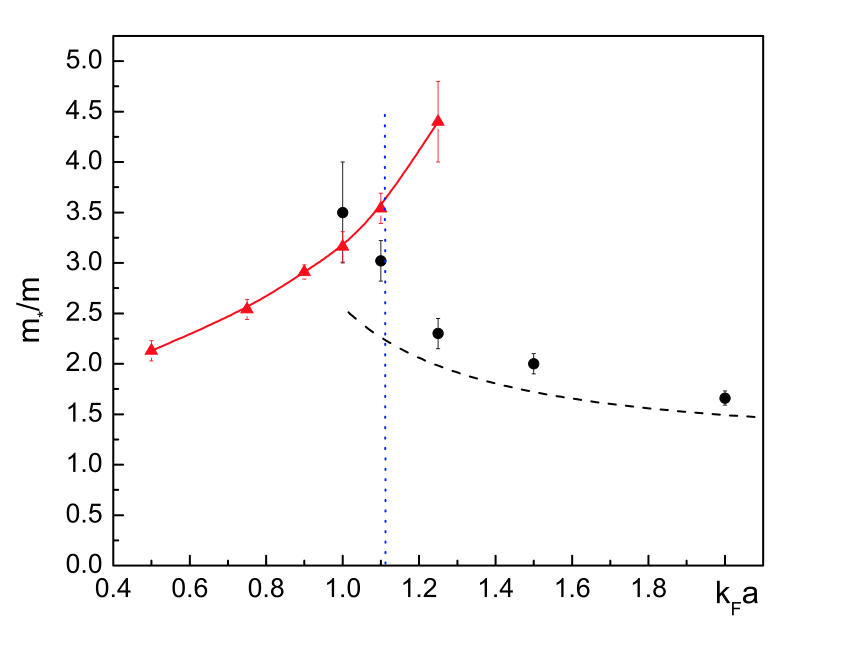
\includegraphics[width=0.7\textwidth]{./intro/chap1MCeffectm.png}
    \bicaption{极化子-分子转变附近极化子与分子的有效质量。其中红色点对应分子有效质量,黑色点对应吸引极化子有限质量,蓝色虚线对应1p-h近似下的转变点。摘自\citep{Prokoffermi}}{Effective mass of polaron and molecule near polaron-molecule transition. Red points for molecule. Black points for polaron. Blue dashed line for polaron-molecule transition point under 1 p-h approximation. Reprinted from\citep{Prokoffermi}}
    \label{MCeffectm}
\end{figure}
%%%%%%%%%%%%%%%%%%%%%%%%%%%%%%%%%%%%%%%%%%%%%%%%%%%%%%%%%%%%%%%%%%%%%%%%%%

在强相互作用区间,远离基态还可以求得方程~\ref{consistentEQ}~一支$E_+>0$的激发态解,随着杂质原子间的相互作用越过共振点,从低能有效散射角度来看杂质原子与背景之间为有效的互相排斥,被称为排斥极化子\cite{Cui2010Stability},在少体物理中对应upper branch,在BEC极限下,我们有$E_{+}=2 \pi a n_{\uparrow} / m_{r}$。

另一方面采用T矩阵单粒子空穴激发近似,计算杂质原子自能也可以得到上述变分波函数相同的自洽方程\cite{Combescot20071ph},令人惊讶的是这样简单的单粒子空穴近似在共振处依然可以成立,其背后的原因在于高阶粒子空穴激发的抵消作用\cite{Combescot20071ph008full}。
%%%%%%%%%%%%%%%%%%%%%%%%%%%%%%%%%%%%%%%%%%%%%%%%%%%%%%%%%%%%%%%%%%%%%%%%%%
\begin{figure}[!htbp]
    \centering
    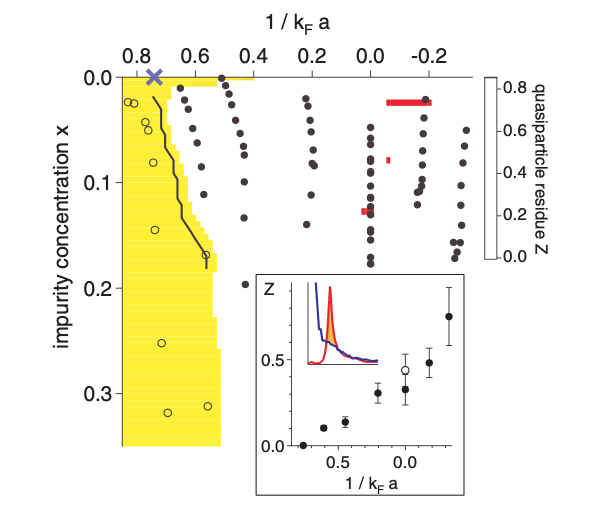
\includegraphics[width=0.6\textwidth]{./intro/chap1fpZ.png}
    \bicaption{准粒子剩余随着相互作用与密度的变化。摘自\citep{Schirotzekobservation}}{Quasiparticle residue as a function of interaction and impurity densuty. Reprinted from \citep{Schirotzekobservation}}
    \label{fpZ}
\end{figure}
%%%%%%%%%%%%%%%%%%%%%%%%%%%%%%%%%%%%%%%%%%%%%%%%%%%%%%%%%%%%%%%%%%%%%%%%%%
实验中费米极化子在非均衡密度的混合费米气体中首先被观测到。其中少数原子成为杂质,多数原子构成背景。杂质原子的单粒子性质被背景费米海上的粒子-空穴激发所重整化。

费米极化子最早的直接实验证据来自MIT研究组\cite{Schirotzekobservation}。实验上制备含有$10^6$个$|1\rangle{}^6$Li原子的体系。然后通过双光子过程将大约$2\%$的$|1\rangle$原子激发到$|3\rangle$。调节$|1\rangle$与$|2\rangle$之间的相互作用,然后通过测量$3|\rangle$到$|2\rangle$的rf谱,通过谱峰的位置来给出极化子的能量,

\begin{comment}
如图~\ref{fpE}~所示。
%%%%%%%%%%%%%%%%%%%%%%%%%%%%%%%%%%%%%%%%%%%%%%%%%%%%%%%%%%%%%%%%%%%%%%%%%%
\begin{figure}[!htbp]
    \centering
    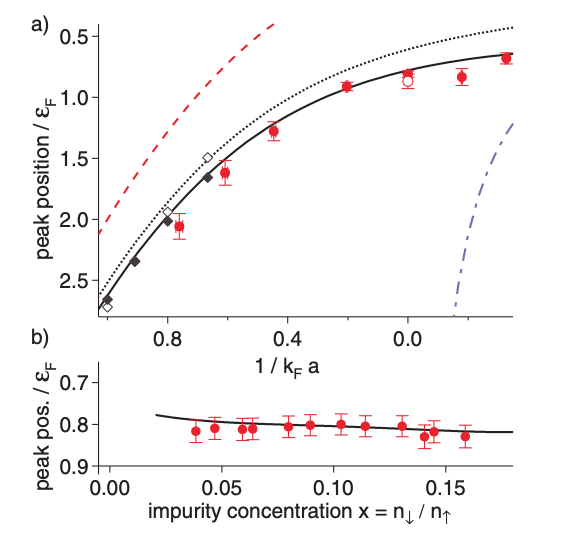
\includegraphics[width=0.7\textwidth]{chap1fpE.png}
    \bicaption{图a为实验测到的(散点)以及理论预测(黑色实线)的费米极化子能量随相互作用变化曲线。图b为rf谱峰的位置随杂质密度的变化。摘自\citep{Schirotzekobservation}}{Fig(a) for measured and predicted energy of fermi polaron upon interaction. Fig(b) for rf spectrum peak position upon impurity densuty. Reprinted from\citep{Schirotzekobservation}}
    \label{fpE}
\end{figure}
%%%%%%%%%%%%%%%%%%%%%%%%%%%%%%%%%%%%%%%%%%%%%%%%%%%%%%%%%%%%%%%%%%%%%%%%%%
可以看到,即使在共振点处,理论计算的能量与实验测到的能量也符合很好。并且谱峰的位置受杂质密度变化影响较小,处于低密度区间。
\end{comment}

分析射频谱的面积,提取出准粒子剩余,如图~\ref{fpZ}~所示,可以看到越过一个临界相互作用,准粒子留数降到了零。这意味着当相互作用越过共振点,极化子能量越来越低,完成基态从极化子到分子的转变。
%%%%%%%%%%%%%%%%%%%%%%%%%%%%%%%%%%%%%%%%%%%%%%%%%%%%%%%%%%%%%%%%%%%%%%%%%%
\begin{figure}[!htbp]
    \centering
    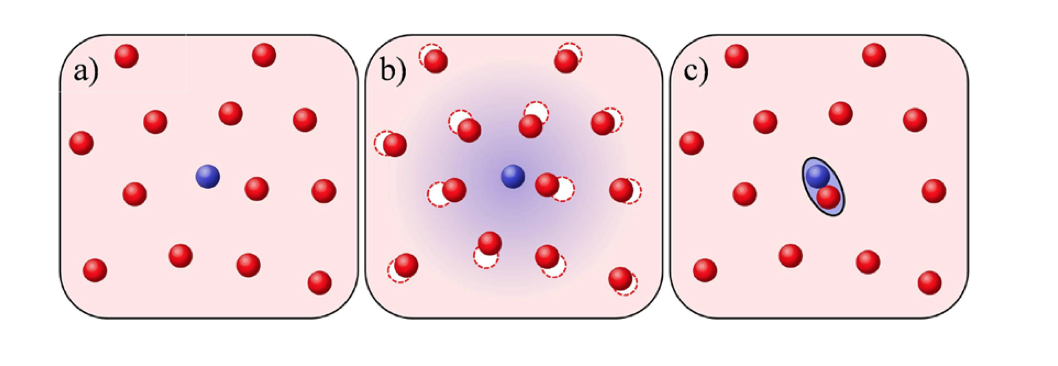
\includegraphics[width=0.7\textwidth]{./intro/chap1fp.png}
    \bicaption{费米极化子的示意图。相互作用从弱变强依次从极化子变到分子。摘自\citep{Schirotzekobservation}}{Illustration of fermi polaron. As interaction goes strong, impurity goes from polaron to molecule. Reprinted from \citep{Schirotzekobservation}.}
    \label{fp}
\end{figure}
%%%%%%%%%%%%%%%%%%%%%%%%%%%%%%%%%%%%%%%%%%%%%%%%%%%%%%%%%%%%%%%%%%%%%%%%%%
进一步实验\cite{kohstall2012metastability}采用不同的体系,制备少量${}^{40}$K与大量${}^{6}$Li的混合气,通过射频脉冲将与Li原子无相互作用的$|0\rangle\equiv\left|F=9 / 2, m_{\mathrm{F}}=-7 / 2\right\rangle$激发到与Li原子有Feshbach共振调节相互作用的$|1\rangle \equiv\left|F=9 / 2, m_{\mathrm{F}}=-5 / 2\right\rangle$。观测到在吸引极化子之上的排斥极化子,如图~\ref{upfp}~所示 :
%%%%%%%%%%%%%%%%%%%%%%%%%%%%%%%%%%%%%%%%%%%%%%%%%%%%%%%%%%%%%%%%%%%%%%%%%%
\begin{figure}[!htbp]
    \centering
    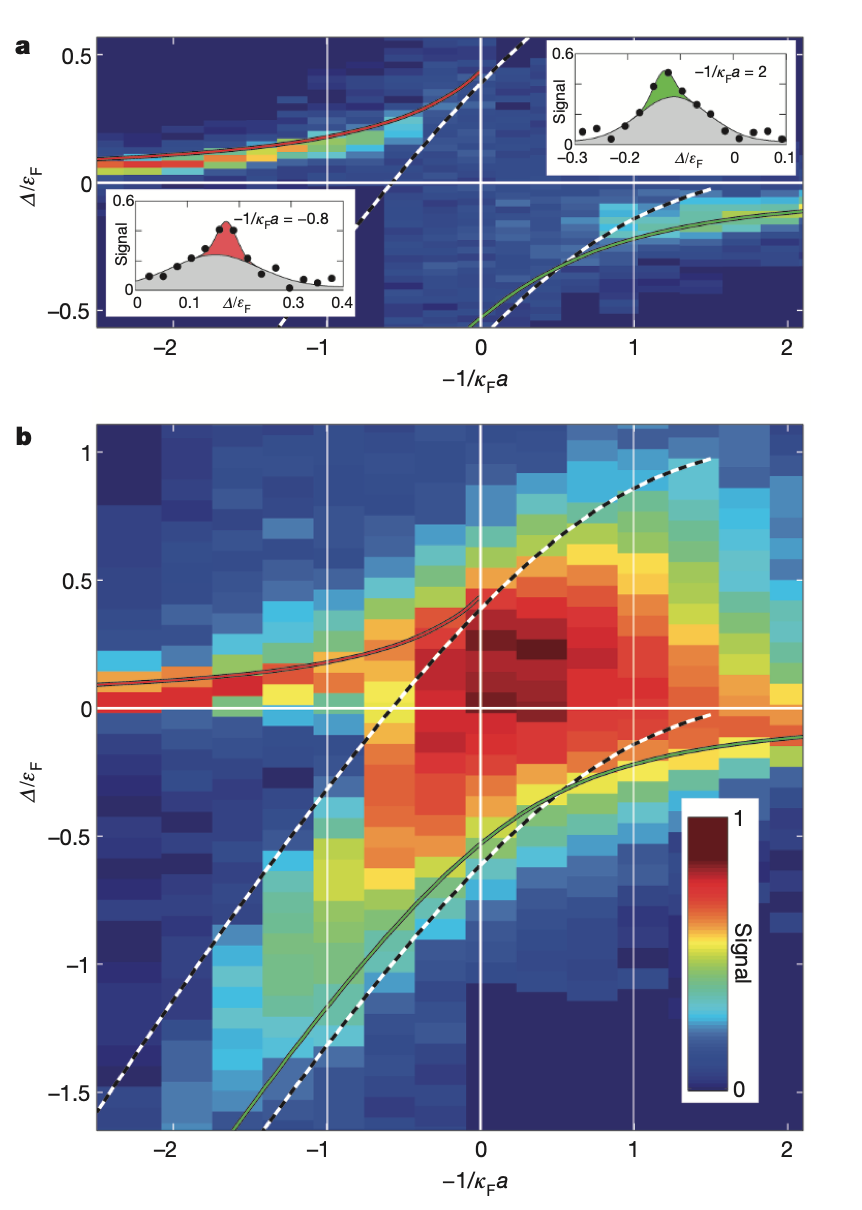
\includegraphics[width=0.6\textwidth]{./intro/chap1upfp.png}
    \bicaption{图a(弱)与b(强)为不同rf场强下测到的吸收谱。可以清楚地看到吸引极化子与排斥极化子两支解,在中间伴有分子态。\citep{kohstall2012metastability}}{Fig a and Fig b for transition spectrum measured under weak and strong rf power. There are attractive polaron branch, repulsive polaron branch ang molecule branch. Reprinted from \citep{kohstall2012metastability}}
    \label{upfp}
\end{figure}
%%%%%%%%%%%%%%%%%%%%%%%%%%%%%%%%%%%%%%%%%%%%%%%%%%%%%%%%%%%%%%%%%%%%%%%%%%
后续在纯${}^{6}$Li体系中也观测到了排斥极化子\cite{Scazzarepulsive}。

\begin{comment}
后续对于排斥极化子对应的极化气体中的铁磁关联也有一定的量子蒙特卡罗数值研究\cite{Conduit2009Inhomo,Pilati2010Itinerant,chang2011ferromagnetism}。除了蒙特卡罗数值以外,通过泛函重整化群也可以得到吸引极化子和排斥极化子的谱密度\cite{Schmidt2011excitation}。

我们知道在低维体系中密度涨落会扮演更重要的角色。那对于二维体系的费米极化子会是如何呢?研究者在${}^{40}$K二维光晶格中实现了二维费米极化子,并观测到了吸引与排斥极化子\cite{koschorreck2012attractive}。
%%%%%%%%%%%%%%%%%%%%%%%%%%%%%%%%%%%%%%%%%%%%%%%%%%%%%%%%%%%%%%%%%%%%%%%%%%
\begin{figure}[!htbp]
    \centering
    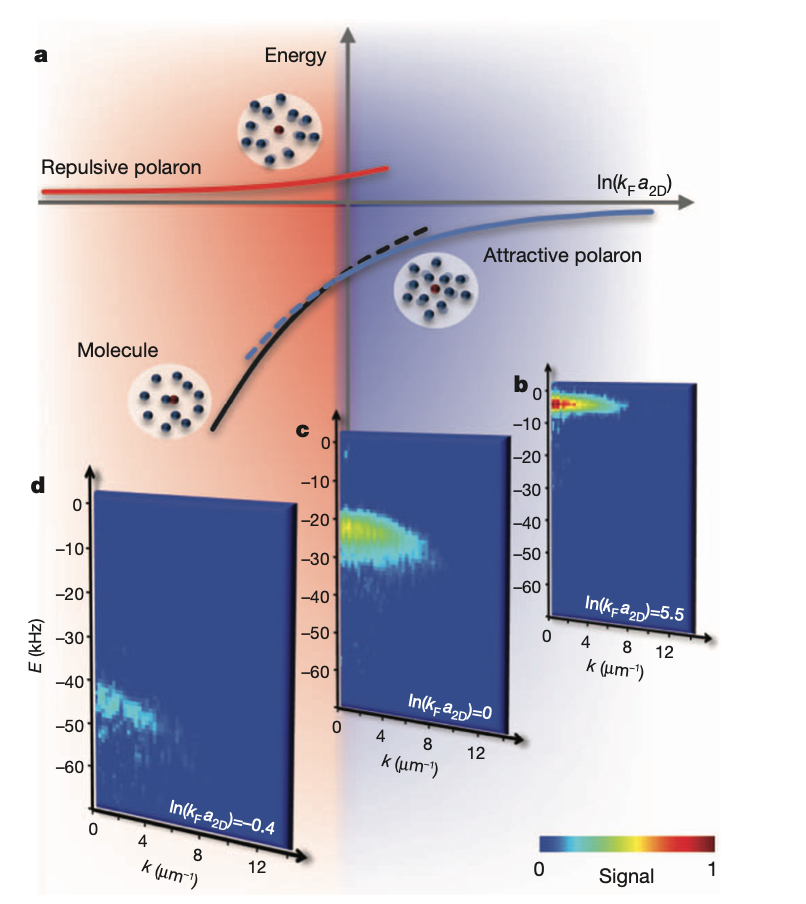
\includegraphics[width=0.7\textwidth]{./intro/chap12dfp.png}
    \bicaption{二维极化子实验观测。排斥极化子、吸引极化子、分子态均被观测到。摘自\citep{koschorreck2012attractive} }{Fermi polaron in 2D, with repulsive branch, attractive branch and molecule. Reprinted from \citep{koschorreck2012attractive} }
    \label{2dfp}
\end{figure}
%%%%%%%%%%%%%%%%%%%%%%%%%%%%%%%%%%%%%%%%%%%%%%%%%%%%%%%%%%%%%%%%%%%%%%%%%%
随着实验技术的成熟,对于极化子探索的方向也有所扩展。比如利用Ramesy相干动力学来研究\cite{Cetina2015decoherence,cetina2016ultrafast}极化子的形成、有限温度下的极化子准粒子性质的破坏\cite{YanBoiling}、以及利用轨道Feshbach共振来调节的极化子等\cite{Darkwah2019}。

%通过改变杂质原子与背景费米子的质量比,我们还可以观察到三聚体的形成\cite{Mathy2011trimers}

在费米极化子实验测量中,最常用的测量手段是rf谱测量。理论上rf谱相应的计算最早来自\cite{Massignan2008Twin},其原理可用简单的三态模型来阐述,制备少量$|1\rangle$态原子与背景$|2\rangle$态原子,之间的相互作用可以调节。然后用rf脉冲将一部分$|1\rangle$态激发到与1,2体系没有相互作用的$|0\rangle$态,rf激发场的哈密顿量为:
\begin{equation}
H_{\mathrm{rf}}=\frac{\Omega}{2} \int \mathrm{d}^{3} r\left[\mathrm{e}^{-\mathrm{i} \omega t} \psi_{1}^{\dagger}(\boldsymbol{r}, t) \psi_{0}(\boldsymbol{r}, t)+\text { h.c. }\right]
\end{equation}
在$|1\rangle$态原子数目很小的情况下,线性响应理论成立,rf场诱导的转化几率随频率变化$R(\omega)$:
\begin{equation}
R(\omega) \propto-\operatorname{Im} \mathcal{D}(\omega) \equiv-\int \mathrm{d}^{3} r \mathrm{~d}^{3} r^{\prime} \operatorname{Im} \mathcal{D}\left(\boldsymbol{r}, \boldsymbol{r}^{\prime}, \omega\right)
\end{equation}
其中$\mathcal{D}(\omega)$为推迟格林函数:
\begin{equation}
G(\boldsymbol{r},\boldsymbol{r}^{\prime},t,t^{\prime}) = -\mathrm{i} \theta\left(t-t^{\prime}\right)\left\langle\left[\psi_{1}^{\dagger}(\boldsymbol{r}, t) \psi_{0}(\boldsymbol{r}, t)\right.\right.\left.\left.\psi_{0}^{\dagger}\left(\boldsymbol{r}^{\prime}, t^{\prime}\right) \psi_{1}\left(\boldsymbol{r}^{\prime}, t^{\prime}\right)\right]\right\rangle
\end{equation}
的傅立叶变换。仅考虑1,2态原子存在相互作用的情况下,可以得到:
\begin{equation}
\begin{split}
&\operatorname{Im} \mathcal{D}(\omega)=-\frac{1}{2} \int \frac{\mathrm{d}^{3} k}{(2 \pi)^{3}} \int \frac{\mathrm{d} \epsilon}{2 \pi}[f(\epsilon)-f(\epsilon+\tilde{\omega})] \\
&\quad \times A_{0}(\boldsymbol{k}, \epsilon) A_{1}(\boldsymbol{k}, \epsilon+\tilde{\omega})
\end{split}
\end{equation}
其中$f(x)=[\exp (\beta x)+1]^{-1}$为费米分布。根据转变的方向可将rf谱分为两类:正向与逆向。初始态仅少量$|1\rangle$原子,rf场将与背景有相互作用的$|1\rangle$原子激发到与背景无相互作用的$|0\rangle$原子,此即正向rf谱。若初始态为少量$|0\rangle$
原子,rf场将与背景无相互作用的$|0\rangle$原子激发到与背景有相互作用的$|1\rangle$原子,此即逆向rf谱。逆向谱的优势在于可以测量整个频率区间的谱相应。

受到实验上对于费米极化子研究的拓展的启发,理论方面也扩展到关于动力学演化与有限温度下费米极化子的研究。基于实验上对Ramesy信号的测量,Parish利用截断粒子空穴的波函数方法\cite{Parish2016quantum}研究Ramesy信号。另一方面基于有限温度极化子实验的启发\cite{YanBoiling},吸引极化子、排斥极化子、分子极化子相变以及rf谱测量谱函数等概念在有限温度下的命运也得到了充分的理论研究,随着温度的升高,极化子的准粒子性质被破坏,相干性降低\cite{tajima2018many,Hu2018attractive,mulkerin2019breakdown,Taylor2019thermal,Liu2020Radio,Liu2020theory,Parish2021thermodynamic}。
\end{comment}

除了上述三维的研究之外,低维情况下的极化子也有很多研究,低维下涨落变得更加重要,任意吸引势下都会存在束缚态。在二维下与三维结论类似:极化子-分子转变依然被认为存在\cite{Zollner2011Polarons,Parish2011pm,Lewenstein2013spinchain012High}。吸引极化子与排斥极化子也存在\cite{Schmidt2012fermi,Ngampruetikorn_2012}。但是在一维下,N+1的体系存在贝特假设严格解\cite{mcguire1965interacting,mcguire1966interacting},变分波函数依然可以给出与贝特假设严格解一致的结果,即一维下不存在极化子到分子的转变\cite{Giraud2009highly,Leskinen_2010,Astrakharchik2013trapped}。

在极化子到分子的转变研究中,对于单极化子来说是个一阶转变。最近通过Raman光谱,研究者进一步揭示了存在有限密度和有限温度下极化子到分子的转变会被连续化\cite{Sagi2020}。通过制备不同内态的${}^{40}$K原子:$|1\rangle$ 作为背景费米海和 $|2\rangle$作为杂质。利用Raman光束将$|2\rangle$激发到$|3\rangle$,跃迁几率是动量依赖的,这是与传统的rf谱很大的不同,收集最终的谱信号并与一定假设下理论预测的Raman能谱去拟合,解析出最终的极化子单粒子性质。其中准粒子剩余如图~\ref{fpsmooth}~所示,可以看到在有限温度以及有限极化子密度下一阶转变变为了连续转变。
%%%%%%%%%%%%%%%%%%%%%%%%%%%%%%%%%%%%%%%%%%%%%%%%%%%%%%%%%%%%%%%%%%%%%%%%%%
\begin{figure}[!htbp]
    \centering
    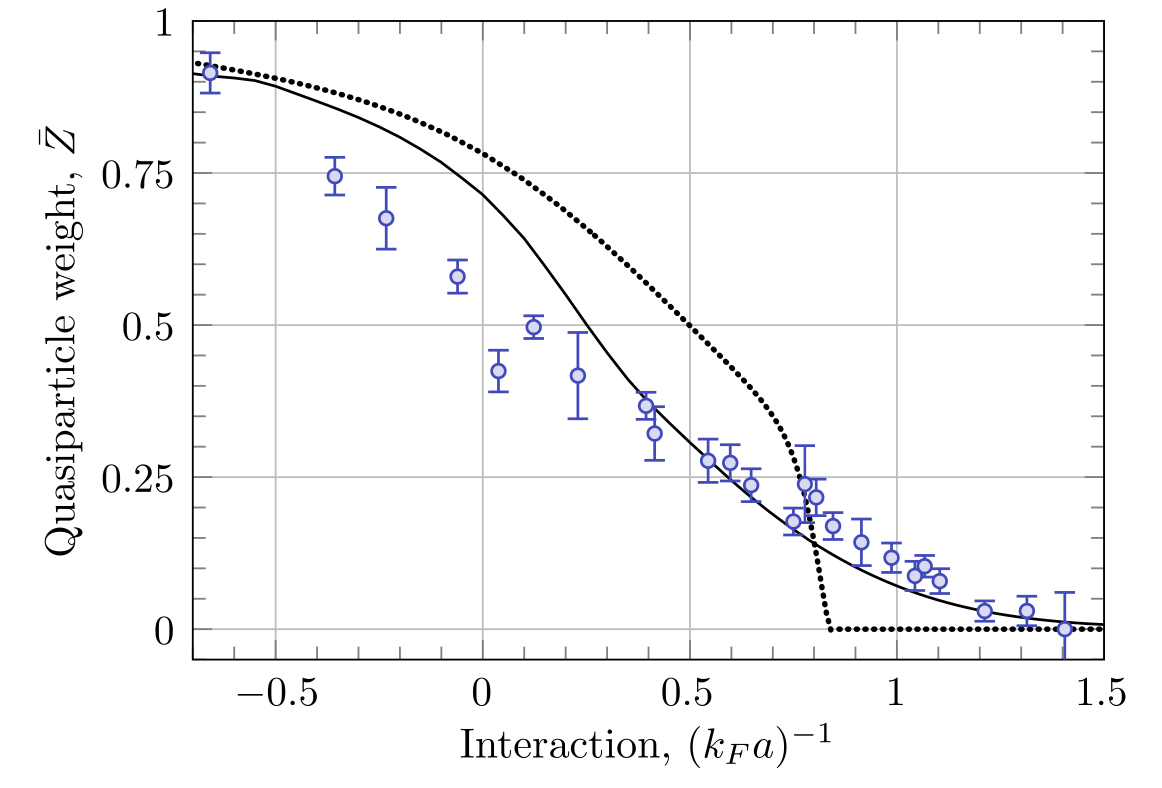
\includegraphics[width=0.7\textwidth]{./intro/chap1smooth.png}
    \bicaption{拟合Raman谱得到的准粒子剩余$Z$,其中散点代表实验观测数据,实线代表LDA近似的结果,点线代表单杂质在$T
    =0$下的准粒子剩余。摘自\citep{Sagi2020}}{Quasiparticle residue obtained from fitting measured Raman Spectrum. Scattered points for experiment results, solid line for LDA results and dotted line for single impurity results at $T=0$. Reprinted from\citep{Sagi2020}}
    \label{fpsmooth}
\end{figure}
%%%%%%%%%%%%%%%%%%%%%%%%%%%%%%%%%%%%%%%%%%%%%%%%%%%%%%%%%%%%%%%%%%%%%%%%%%




\section{本征热化假说}\label{1sec:ETH}
热化一直是统计物理中很基础的概念。统计物理中(经典或者量子)宏观数目自由度体系在到达热力学平衡态之后,体系热力学性质可以仅用几个参数来描述(如温度、压强、化学势等),宏观可观测量由热力学统计分布给出。为什么宏观体系可以仅用几个参数来描述?宏观体系是如何到达热力学平衡态的?如何在量子力学的层面去理解这一热化现象?基于这些非常基本的问题,用来理解量子系统热化现象的假说——本征热化假说被提出。我们在这一节中详细介绍一下目前的研究进展。更加详细的讨论参见\cite{d2016quantum,deutsch2018eigenstate}。

一个孤立体系的量子力学的演化是幺正的,从初态出发,初态在不同本征态上的权重是不随时间变化的。但是最终随着长时间的演化,系统的宏观可观测量不依赖于初态的权重分布。仅有几个参数所确定。此时一个自然的想法被提出来———本征热化假说\cite{Deutsch1991quantum,Srednicki1994chaos,srednicki1999approach}。其核心思想为对于能量处于$\bar{E}=\langle\psi_I|\hat{H}|\psi_I\rangle$附近的本征态,其局域算符的平均值是一样的。我们用形式化的语言来表述,考虑一个孤立系统$\hat{H}$,本征态于本征能量:$\hat{H}|m\rangle=E_m|m\rangle$。从任意初态出发时间演化得到t时刻波函数:
\begin{equation}
|\psi(t)\rangle=\sum_{m} C_{m} \mathrm{e}^{-i E_{m} t}|m\rangle
\end{equation}
其中$C_m = \langle m | \psi_I\rangle$,出于方便我们取$\hbar=1$。对某个局域算符可观测量$\hat{O}$来说,t时刻观测期望值为:
\begin{equation}
\begin{aligned}
O(t) & \equiv\langle\psi(t)|\hat{O}| \psi(t)\rangle=\sum_{m, n} C_{m}^{*} C_{n} e^{i\left(E_{m}-E_{n}\right) t} O_{m n} \\
&=\sum_{m}\left|C_{m}\right|^{2} O_{m m}+\sum_{m, n \neq m} C_{m}^{*} C_{n} e^{i\left(E_{m}-E_{n}\right) t} O_{m n}
\end{aligned}
\end{equation}
其中$O_{m n}=\langle m|\hat{O}| n\rangle$。如果体系最终热化,则局域算符的长时间平均应该等于微正则系综平均,并且$O(t)$的长时间行为应该围绕这一平均值做热力学涨落。此时根据本征热化假说,对于热化的体系,$O_{mn}$满足:
\begin{equation}
O_{m n}=O(\bar{E}) \delta_{m n}+e^{-S(\bar{E}) / 2} f_{O}(\bar{E}, \omega) R_{m n}
\end{equation}
其中$\bar{E} \equiv\left(E_{m}+E_{n}\right) / 2, \omega \equiv E_{n}-E_{m}$。$S(E)$是能量为E时候的热力学熵。$O(\bar{E})$与$f_{O}(\bar{E}, \omega)$为光滑单值函数。$R_{m n}$为随机变量,满足$\overline{\left|R_{m n}\right|^{2}}=1$。这一假设目前没有严格的证明。但是有很多数值上的验证。其中对角元部分与长时间平均值有关,非对角元部分则与围绕平均值的涨落有关。考虑$O(t)$的长时间平均,在这里我们考虑广义的封闭系统,将对称性考虑进去之后,系统没有简并,这个假设是合理的,因此:
\begin{equation}
\bar{O} \equiv \lim _{t_{0} \rightarrow \infty} \frac{1}{t_{0}} \int_{0}^{t_{0}} d t O(t)=\sum_{m}\left|C_{m}\right|^{2} O_{m m}=\operatorname{Tr}\left[\hat{\rho}_{\mathrm{DE}} \hat{O}\right]
\end{equation}
其中$\hat{\rho}_{DE}$为对角系综。我们定义初态的能量方差为:
\begin{equation}
\delta E \equiv \sqrt{\left\langle\psi_{I}\left|\hat{H}^{2}\right| \psi_{I}\right\rangle-\left\langle\psi_{I}|\hat{H}| \psi_{I}\right\rangle^{2}}
\end{equation}
如果方差很小,那么就会有:
\begin{equation}
\bar{O} \simeq O(\langle E\rangle) \simeq O_{\mathrm{ME}}
\end{equation}
进一步,我们量化这一差异,考虑泰勒展开:
\begin{equation}
O_{m m} \approx O(\langle E\rangle)+\left.\left(E_{m}-\langle E\rangle\right) \frac{d O}{d E}\right|_{\langle E\rangle}+\left.\frac{1}{2}\left(E_{m}-\langle E\rangle\right)^{2} \frac{d^{2} O}{d E^{2}}\right|_{\langle E\rangle}
\end{equation}
将其带入长时间平均得到:
\begin{equation}
\bar{O} \approx O(\langle E\rangle)+\frac{1}{2}(\delta E)^{2} O^{\prime \prime}(\langle E\rangle) \approx O_{\mathrm{ME}}+\frac{1}{2}\left[(\delta E)^{2}-\left(\delta E_{\mathrm{ME}}\right)^{2}\right] O^{\prime \prime}(\langle E\rangle)
\end{equation}
其中$\delta_{ME}$为微正则系综的能量涨落标准差。而对于仅有局域相互作用的孤立系统来说$\delta E$为:
\begin{equation}
\begin{array}{r}
\delta E \equiv \sqrt{\langle\psi_{I}|\hat{H}^{2}| \psi_{I}\rangle-\langle\psi_{I}|\hat{H}| \psi_{I}\rangle^{2}}=\sqrt{\langle\psi_{I}|\hat{H}_{1}^{2}| \psi_{I}\rangle-\langle\psi_{I}|\hat{H}_{1}| \psi_{I}\rangle^{2}} \\
=\sqrt{\sum_{j_{1}, j_{2}}\left[\langle\psi_{I}|\hat{h}_{j_{1}} \hat{h}_{j_{2}}| \psi_{I}\rangle-\langle\psi_{I}|\hat{h}_{j_{1}}| \psi_{I}\rangle\langle\psi_{I}|\hat{h}_{j_{2}}| \psi_{I}\rangle\right]}
\end{array}
\end{equation}
其中$\hat{H}=\hat{H}_{0}+\hat{H}_{1}$,$\hat{H}_{1}=\sum_{j} \hat{h}_{j}$仅有局域关联的算符。因此通常情况下有:
\begin{equation}
\delta E \sim \sqrt{V}
\end{equation}
继而有$\delta E / E \sim 1 / \sqrt{V}$。因此这一差异在热力学极限下趋近于0。

我们然后计算局域算符平方的长时间涨落:
\begin{equation}
\begin{aligned}
\sigma_{O}^{2} & \equiv \lim _{t_{0} \rightarrow \infty} \frac{1}{t_{0}} \int_{0}^{t_{0}} d t[O(t)]^{2}-(\bar{O})^{2} \\
&=\lim _{t_{0} \rightarrow \infty} \frac{1}{t_{0}} \int_{0}^{t_{0}} d t \sum_{m, n, p, q} O_{m n} O_{p q} C_{m}^{*} C_{n} C_{p}^{*} C_{q} \mathrm{e}^{i\left(E_{m}-E_{n}+E_{p}-E_{q}\right) t}-(\bar{O})^{2} \\
&=\sum_{m, n \neq m}\left|C_{m}\right|^{2}\left|C_{n}\right|^{2}\left|O_{m n}\right|^{2} \leq \max \left|O_{m n}\right|^{2} \sum_{m, n}\left|C_{m}\right|^{2}\left|C_{n}\right|^{2}=\max \left|O_{m n}\right|^{2} \propto \exp [-S(\bar{E})]
\end{aligned}
\end{equation}
可以看到这一涨落由非对角元控制,且随系统体积被指数压低。我们接着去看局域算符涨落的方差:
\begin{equation}
\overline{\delta O^{2}}=\lim _{t_{0} \rightarrow \infty} \frac{1}{t_{0}} \int_{0}^{t_{0}} d t\left\langle\psi(t)\left|(\hat{O}-\bar{O})^{2}\right| \psi(t)\right\rangle=\sum_{m}\left|C_{m}\right|^{2}\left(O^{2}\right)_{m m}-\bar{O}^{2}
\end{equation}
同样也有:
\begin{equation}
\sqrt{\overline{\delta O^{2}}} / \bar{O} \simeq \sqrt{\delta O_{\mathrm{ME}}^{2}} / O_{\mathrm{ME}} \simeq 1 / \sqrt{V}
\end{equation}
由以上分析,我们可以理解,在本征热化假设成立的前提下,孤立系统局域算符的长时间平均等于热力学吉布斯平均(包括微正则、正则与巨正则系综)。那么本征热化假设有哪些成立的证据呢?目前来讲证据主要来自于格点系统的数值模拟。主要的模型包括硬核玻色子模型\cite{rigol2008thermalization,Santos2010Localization,Rigol2009Breakdown,Rigol2010Quantum,Neuenhahn2012Thermalization,Steinigeweg2013Eigenstate,Kim2014testing,beugeling2014finite,Steinigeweg2014Pushing,Khodja2015Relevance,Beugeling2015Off-diagonal}以及横场伊辛模型\cite{Fratus2015Eigenstate,Mondaini2016Eigenstate,Mondaini2017Eigenstate,blass2016test,Serbyn2013local}。我们挑选其中有代表性工作介绍,如图~\ref{ETHnum}~所示,展示了一维硬核玻色子与带纵场的横场伊辛模型的数值结果\cite{Kim2014testing}。可以看到对角元部分随着系统尺寸的增大局域算符的本征态期望值逐渐收敛到与能量有关的单值函数。
%%%%%%%%%%%%%%%%%%%%%%%%%%%%%%%%%%%%%%%%%%%%%%%%%%%%%%%%%%%%%%%%%%%%%%%%%%
\begin{figure}[!htbp]
    \centering
    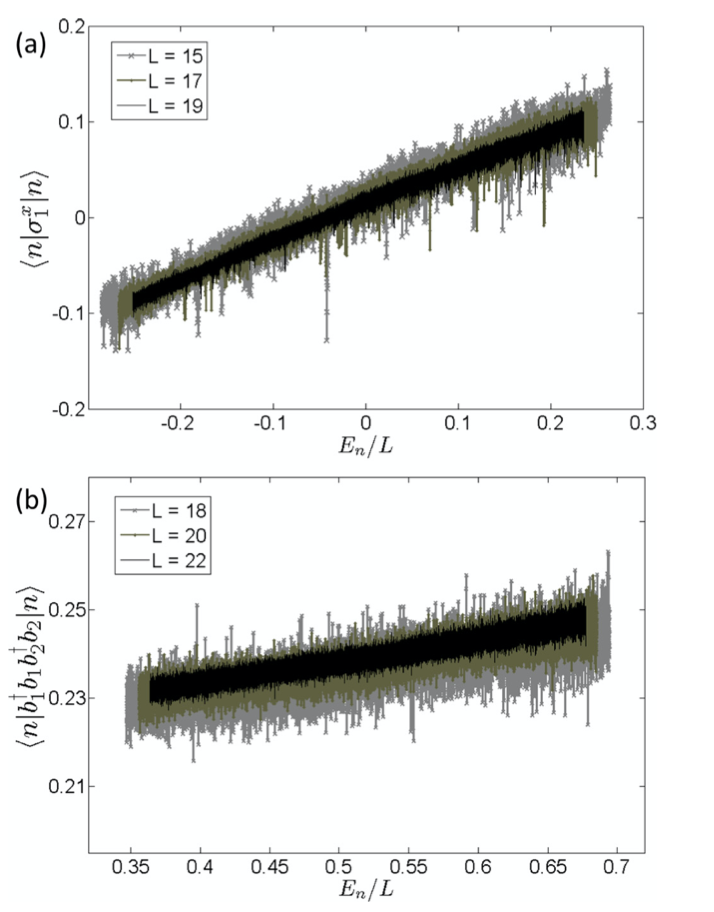
\includegraphics[width=0.7\textwidth]{./intro/chap1ETHnum.png}
    \bicaption{局域算符的对角元随本征能量的分布。其中(a)为带纵场的横场伊辛模型。(b)为带有次近邻相互作用的硬核玻色子模型。 摘自\citep{Kim2014testing}}{Eigenstate expectation value of local operators vs eigen energy. Fig (a) for TFIM with longitudinal filed and Fig (b) for hard core bosons with next-nearest-neighbor interaction. Reprinted from\citep{Kim2014testing}}
    \label{ETHnum}
\end{figure}
%%%%%%%%%%%%%%%%%%%%%%%%%%%%%%%%%%%%%%%%%%%%%%%%%%%%%%%%%%%%%%%%%%%%%%%%%%
而对于非对角元部分的验证也有部分数值验证,不过还尚未成熟,可以参见\cite{Beugeling2015Off-diagonal,Mondaini2017Eigenstate}。

本征热化假说(ETH)本身以及其数值证据,吸引着越来越多研究者的注意。但这一假说是个要求很强的假说。随着研究者对此认识的不断加深,越来越多的违背本征热化假说的系统被发现。其中以量子可积系统\cite{kinoshita2006quantum,Rigol2007Relaxation,Calabrese2011Quantum,essler2016quench,vidmar2016generalized}与多体局域化系统\cite{basko2006metal,Serbyn2013local,Huse2014Phenomenology}最为典型,这两种体系是完全的本征热化假说破缺的体系,并且得到了实验的验证。


除了这种完全违背本征热化假说的系统,随着实验手段的进步,最近在实验中发现了弱违背本征热化假说的体系,其中以量子多体伤痕为典型例子。量子多体伤痕最早来源于里德堡原子的实验,在51个原子的一维链中,观测到$|Z_2\rangle$初态出发的反常动力学,其长时间震荡行为与长时间平均值均表明非热化的发生\cite{bernien2017probing}。如图所示~\ref{scar}~。
%%%%%%%%%%%%%%%%%%%%%%%%%%%%%%%%%%%%%%%%%%%%%%%%%%%%%%%%%%%%%%%%%%%%%%%%%%
\begin{figure}[!htbp]
    \centering
    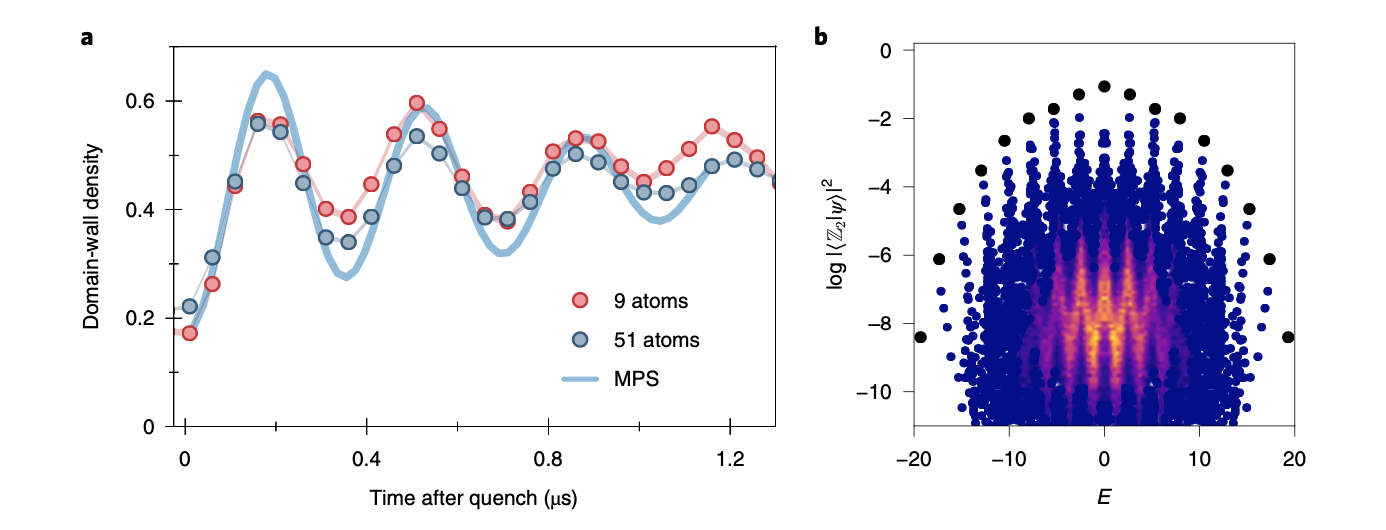
\includegraphics[width=0.7\textwidth]{./intro/chap1scar.png}
    \bicaption{图a为里德堡实验平台观察到的量子多体伤痕动力学,图b为后续通过与$|Z_2\rangle$做投影筛选得到非热化子空间。摘自\citep{bernien2017probing,serbyn2021quantum}}{Fig a for many body scar dynamics from Rydberg atoms simulation and Fig b for non-thermalized sub Hilbert space obtained from overlap with $|Z_2\rangle$. Reprinted from\citep{bernien2017probing,serbyn2021quantum}}
    \label{scar}
\end{figure}
%%%%%%%%%%%%%%%%%%%%%%%%%%%%%%%%%%%%%%%%%%%%%%%%%%%%%%%%%%%%%%%%%%%%%%%%%%
对这一实验的理论研究表明,反常动力学存在的原因为本征态希尔伯特空间中近似分立的子空间,其维度正比于链长。这一子空间在可以通过与初态$|Z_2\rangle$做投影,或者计算局域算符的本征态期望值,或者计算本征态的半链纠缠熵挑选出来\cite{turner2018weak,Turner2018quantum,Ho2019periodic,Choi2019emergent,Michailidis2020slow,serbyn2021quantum},如图~\ref{scar}~所示。

围绕着本征热化假说,孤立体系的热化的神秘面纱被逐步揭开。伴随着量子模拟实验技术的进步,我们对于热化的了解也会越来越深入下去,但是同样的未知也在逐步增多,这仍是一个在蓬勃发展的领域。





\section{本文安排}\label{1sec:sum}
在接下来的章节中,我们首先在第~\ref{chap:kondo}~章中从相对简单的少体磁性杂质体系出发,考虑一维下局域自旋与两个巡游费米子之间在自旋交换相互作用影响下的能谱结构,揭示少体体系的基态与激发态中蕴藏的特殊少体关联行为。然后转入第~\ref{chap:polaron}~章,我们从少体杂质体系来到多体杂质的研究。我们考虑典型的费米极化子物理,采用统一的变分波函数研究基态从极化子到分子的转变,揭示这一转变的本质在于基态从零动量到费米动量的转移,讨论维度与泡利禁闭机制在这一转变中发挥的作用。并且基于转变点附近的极化子与分子共存机制讨论了实验体系中有限温度和有限密度对单粒子观测量的连续化影响。在第~\ref{chap:ETH}~章我们从能谱的静态行为转变到动力学行为研究,系统地考察带有纵场的横场伊辛模型中,从固定初态出发,选取不同的耦合参数计算局域算符的时间平均与热力学系综平均得到热化的相图。在第~\ref{chap:sum}~章总结并展望这一从少体到多体再到动力学的研究脉络,这有助于我们对量子体系新奇物理特性理解的深入。



%\chapter{自旋交换相互作用体系少体精确解}\label{chap:kondo}

受到最近在超冷碱土金属平台中模拟近藤物理的实验以及理论进展的启发,采用严格对角化的数值方法,我们精确地研究了一维谐振子势场下一个局域磁性杂质与一个以及两个巡游费米子在自旋交换相互作用支配下的1+1以及1+2少体体系的能谱结构。在1+1少体体系中,我们发现对应于不同的铁磁、反铁磁耦合,少体精确解中的attractive branch与repulsive branch具有不同的磁性结构。对于1+2少体体系,在反铁磁耦合下的attractive branch中我们发现了类似于多体物理中的近藤屏蔽效应。进一步地,我们在反铁磁耦合体系中发现了一系列铁磁repulsive branch,它们与其他的attractive branch正交,并且其波函数拥有良好的自旋电荷分离的特点。最后,我们还简单探讨了实际体系中经常带有的接触相互作用带来的影响以及向多体体系的推广。我们的结果尝试从少体的角度发觉带有自旋交换相互作用影响的体系所独有的内禀物理特性,并期待可以在未来的超冷原子实验中得到实现与探索。

在~\ref{sec:spex-intro}~节中,我们介绍这一工作的背景和动机。在~\ref{sec:spex-model}~节中,我们介绍考虑的少体模型以及求解的数值方法。在~\ref{sec:spex-result}~节中,我们讨论得到结果并揭示其物理图像。在~\ref{sec:spex-summary}~节中,我们总结我们的结果并做后续研究的展望。

\section{引言}\label{sec:spex-intro}
在本论文的第一章里面~\ref{sec:spin-exchange}~中我们系统的介绍了自旋交换相互作用在超冷碱土金属原子中的研究进展。总体来讲,利用最外层2个电子的中性原子的基态${}^1S_0$与激发态${}^3P_0$来组成两轨道体系,整个原子的核自旋作为每个粒子的自旋自由度。不同轨道之间的自旋交换相互作用由实验所证实,其中裸的铁磁交换相互作用由${}^{173}$Yb\cite{scazza2014observation,cappellini2014direct,pagano2015strongly,hofer2015observation}与${}^{87}$Sr\cite{zhang2014spectroscopic}原子实现,而裸的反铁磁交换相互作用由${}^{171}$Yb\cite{ono2019antiferromagnetic}原子实现。通过使用束缚诱导共振技术,我们可以方便地低维度下体系的自旋交换相互作用的强度。这种调节已由理论和实验所证实\cite{zhang2016kondo,cheng2017enhancing,zhang2018control,ji2018confinement,zhang2020tight,zhang2020controlling,riegger2018localized}。进一步地,在近藤物理模拟中起关键作用的局域磁性杂质可以借由“魔法”频率光晶格来实现,其原理在于选取合适频率的激光形成光晶格,这种特殊的光晶格利用不同原子态的交流极化率来有选择性的使${}^3P_0$态的原子被束缚住,而${}^1S_0$态的原子则可以自由运动\cite{riegger2018localized,barber2008optical}。上述实验技术与理论计算的进展使得冷原子平台模拟多体近藤物理不再遥远。

不止于此,基于目前的研究进展,我们发现已经可以将目光聚集在少体体系。不同于多体体系,少体体系其独有的理论精确解为理解其中的物理提供坚实的基础。其中简洁的物理图像不仅为少体体系独有,而且为理解与表征多体体系提供丰富的线索。在本文的~\ref{sec:fewbody}~里面我们讨论了相关的背景,{\color{red} 待补充 }


综上,我们发现带有自旋交换相互作用的少体体系亟需系统的研究。因此在这一章节中,我们采用严格对角化的数值方法,系统地求解了1维简谐势场下带有自旋交换相互作用的1+N少体体系:
\begin{equation}\label{eq:sp-ex}
    \adddotsbeforeeqnnum%
    \hat{U}_{ex} = J\cdot\sum_{j=1}^{N}\hat{\Vector{S}}_j\cdot\hat{\Vector{S}}\cdot \delta(x_j)
\end{equation}
其中前面的1为局域带自旋1/2的磁性杂质(自旋算符为$\hat{\Vector{S}}$),位于原点处。后部面的N代表带自旋1/2的巡游费米子(自旋算符为$\hat{\Vector{S}}_j$),在本文中我们研究$N=1,2$。我们考虑杂质与费米子之间各向同性的铁磁与反铁磁海森堡耦合,其耦合强度可以调节。早在1980年代,描述一维连续空间里的费米子与局域自旋杂质体系的多体近藤模型就可用贝特假设的办法严格求解\cite{andrei1983solution},不过其前提在于假设费米子的色散关系为线性($\epsilon_k\propto k$),并带有可重整化的cut off。在这个假设下得到的结果,只有当费米海附近的费米子被自旋杂质散射时才成立,这对应若耦合极限附近。作为对比,在我们这一章节讨论当中,我们求解从弱到强整个相互作用区间的少体能谱与波函数,旨在得到系统的少体物理结果,为多体体系的研究提供启发。


最终,我们的结果总结如下:在自旋交换相互作用支配下的少体体系,展示了不同于纯接触相互作用少体体系的新奇特性。attractive 与 repulsive branch 的磁性结构由自旋交换的铁磁$J<0$与反铁磁$J>0$所决定。重要地,对于1+2的少体体系,我们发现对于反铁磁耦合,基态的attractive branch展现出一种屏蔽效应,而铁磁耦合的attractive branck则没有这种屏蔽。进一步,我们在反铁磁耦合这边发现了一系列的铁磁upper branch激发态,这些特殊的铁磁branch与其它的attractive branch没有发生level avoid crossing,其波函数具有很好的自旋电荷分离的特性。这些新奇的现象都来自于自旋交换相互作用,相应的branch也很容易在碱土金属原子实验中去探测,最后我们还考虑了实际体系经常伴有的纯接触相互作用的影响,以及简单的从少体物理特性到多体物理特性的推广。

\section{模型与计算}\label{sec:spex-model}
我们首先详尽的给出考虑的1+1与1+2少体体系的哈密顿量,并结合具体的物理意义给出变分波函数,最终推导出用于数值求解的矩阵方程。
\subsection{1+N体系哈密顿量}
我们的1+N少体体系处于一维简谐势场中,一个局域的自旋杂质被固定在原点$x=0$处,仅有自旋自由度,空间自由度被冻结。N个巡游费米子在一维连续空间运动,坐标表象下其位置为$x_j,j=1,...,N$。巡游费米子与局域自旋杂质之间存在自旋交换相互作用,整个体系的哈密顿量为(我们在本章中取$\hbar=1$):
\begin{equation}\label{eq:spex-hamiltonian}
\adddotsbeforeeqnnum%
    \begin{split}
       	\hat{H}  &= \hat{H}_0 + \hat{U}_{ex}\\
		\hat{H}_0 &= \sum_{j=1}^{N} \left( -\frac{1}{2M} \frac{\partial^2}{\partial x_{j}^2}   +\frac{M\omega^2}{2}x_{j}^2 \right); \\
		\hat{U}_{ex} &= 2J\cdot\sum_{j=1}^N\delta(x_j){\hat{\Vector{S}}}_j\cdot {\hat{\Vector{S}}}.
    \end{split}
\end{equation}
其中$M$为巡游费米子的质量,$\omega$为谐振子的特征频率,$\hat{\Vector{S}}=(\hat{S}_{x},\hat{S}_{y},\hat{S}_{z})$与$\hat{\Vector{S}}_j=(\hat{S}_{jx},\hat{S}_{jy},\hat{S}_{jz})$分别代表杂质与费米子自旋算符。展开为产生湮灭场算符为:
\begin{equation}\label{eq:spex-field}
\adddotsbeforeeqnnum%
    \begin{split}
		\hat{S}_{jx} &= \frac{1}{2}(\hat{\psi}_{\uparrow}^{\dag}(x_j)\hat{\psi}_{\downarrow}(x_j)+\hat{\psi}_{\downarrow}^{\dag}(x_j)\hat{\psi}_{\uparrow}(x_j));\\
		\hat{S}_{jy} &= \frac{-i}{2}(\hat{\psi}_{\uparrow}^{\dag}(x_j)\hat{\psi}_{\downarrow}(x_j)-\hat{\psi}_{\downarrow}^{\dag}(x_j)\hat{\psi}_{\uparrow}(x_j));\\
		\hat{S}_{jz} &= \frac{1}{2}(\hat{\psi}_{\uparrow}^{\dag}(x_j)\hat{\psi}_{\uparrow}(x_j)-\hat{\psi}_{\downarrow}^{\dag}(x_j)\hat{\psi}_{\downarrow}(x_j)).
    \end{split}
\end{equation}
其中$\hat{\psi}_{\sigma}^{\dag}(x)$为在x处产生一个自旋为$\sigma(\uparrow,\downarrow)$的费米子产生算符。在谐振子基矢下其展开式为:
\begin{equation}
\adddotsbeforeeqnnum%
	\hat{\psi}_{\sigma}^{\dag}(x)=\sum_m \hat{C}_{m\sigma}^{\dag} \phi_m(x).
\end{equation}
其中$\hat{C}_{m\sigma}^\dagger$是产生一个处于第$m$个简谐振子能级的带有自旋$\sigma$费米子的产生算符,该能级的本征波函数在坐标表象下记为$\hat{\phi}_m(x)$,本征能量为$E_m = (m+\frac{1}{2})\omega$。在这套完备的谐振子基矢下系统的哈密顿量(\ref{eq:spex-hamiltonian})可以重新写为二次量子化形式:
\begin{equation}
	\begin{split}
		\hat{H} &= \sum_{m\sigma}E_m \hat{C}_{m\sigma}^\dagger \hat{C}_{m\sigma} + \sum_{m,n} \hat{V}_{mn} ( \hat{C}_{m\uparrow}^\dagger  \hat{C}_{n\downarrow} \hat{S}_- + h.c. \\
     	& +   (\hat{C}_{m\uparrow}^\dagger  \hat{C}_{n\uparrow}-\hat{C}_{m\downarrow}^\dagger  \hat{C}_{n\downarrow}) \hat{S}_{z} ), \label{eq:H2}\\
\end{split}
\end{equation}
其中$V_{mn} = J\phi_m(0)\phi_n(0)$是自旋交换相互作用$\hat{V}_{ex}$导致的$m,n$本征态之间跃迁的矩阵元。我们记$|\Uparrow\rangle$ 与$|\Downarrow\rangle$为局域杂质的自旋态,因此我们有$S_+=|\Uparrow\rangle\langle \Downarrow|$,$S_-=|\Downarrow\rangle\langle \Uparrow|$,而$S_z=(|\Uparrow\rangle\langle \Uparrow|-|\Downarrow\rangle\langle \Downarrow|)/2$。我们可以清楚得看到自旋交换过程是由(\ref{eq:H2})中括号里面的前两项实现的。

接下来我们给出用于具体求解少体能谱的计算公式。包括1+1与1+2自旋交换作用少体体系。

\subsection{一个杂质与一个费米子}
由于哈密顿量(\ref{eq:H2})依然具有自旋$SU(2)$旋转对称性。1+1少体体系按照一个杂质与一个费米子系统总的自旋$\hat{\Vector{S}}_{tot}$划分为自旋三重态通道($\hat{\Vector{S}}_{tot}=1$)与自旋单重态通道($\hat{\Vector{S}}_{tot}=0$)。每个独立的通道都是自旋算符的本征态。因此我们有每个通道的有效描述:
\begin{equation}
U_{s,t}(x_1)=\gamma_{s,t}\delta(x_1).
\end{equation}
其中单重态($singlet$)通道下费米子与杂质的有效耦合强度为$\gamma_s = \frac{-3J}{2}$,三重态($triplet$)通道下费米子与杂质的有效耦合强度为$\gamma_t = \frac{J}{2}$。

为了在同一个变分波函数中包含单重态通道与三重态通道的共同表达式,我们将波函数取在($S_{tot,z}=0$)的封闭子希尔伯特空间中:
\begin{equation}
	|\Psi\rangle_2=\sum_m \left( \phi_m^1 \hat{C}_{m\uparrow}^\dagger|0\rangle \Downarrow+ \phi_m^2 \hat{C}_{m\downarrow}^\dagger|0\rangle \Uparrow \right).
\end{equation}
其中$|0\rangle$是具有0个费米子的真空态。将波函数带入到薛定谔方程:
\begin{equation}
	\hat{H} |\Psi \rangle_2 = E |\Psi\rangle_2,
\end{equation}
我们得到如下的耦合方程组
\begin{equation}
    \begin{split}
      (E-E_m) \phi^1_m &= \sum_p (V_{mp}\phi^2_p-\frac{1}{2}V_{mp}\phi^1_p )\\
      (E-E_m) \phi^2_m &= \sum_p (V_{mp}\phi_p^1 -\frac{1}{2}V_{mp}\phi^2_p).
    \end{split}
\end{equation}
我们从中可以看到这组耦合方程有两类解,其中一类是:
\begin{equation}
    \phi^1_m=\phi^2_m \propto \frac{\phi_m(0)}{E-E_m},
\end{equation}
容易发现,这类解对应的是一个自旋三重态,其能量$E(=E_t)$满足自洽方程:
\begin{equation}
      \frac{1}{\gamma_t} =  \sum_m \frac{|\phi_m(0)|^2}{E_t-E_m}. \label{eq_t}
\end{equation}
而另一类解对应的是一个自旋单重态:
    \begin{equation}
      \phi^1_m = -\phi^2_m\propto \frac{\phi_m(0)}{E_s-E_m},
    \end{equation}
其能量$E(=E_s)$满足自洽方程:
	\begin{equation}
      \frac{1}{\gamma_s} =  \sum_m \frac{|\phi_m(0)|^2}{E_s-E_m}. \label{eq_s}
    \end{equation}
进一步地,两个自洽方程(\ref{eq_t},\ref{eq_s})可以统一为一个方程:
    \begin{equation}
        -\frac{2\sqrt{\pi}}{\kappa_{s,t}} = B(-\frac{\rho_{s,t}}{2},\frac{1}{2}) 
    \end{equation}
其中$\kappa_{s,t} \equiv \gamma_{s,t}\sqrt{M/\omega}$, $\rho_{s,t} \equiv E_{s,t}/\omega-1/2$,而$B(x,y)$是特殊函数中的贝塔函数。

\subsection{一个杂质与两个费米子}
有了1+1体系的求解,我们进一步考虑如果再增加一个自由费米子变成1+2体系,会出现如何有趣的物理呢?对于1个杂质和2个费米子的三体体系,系统总的自旋$\hat{\Vector{S}}_{tot}$可以为$\hat{\Vector{S}}_{tot}=1/2$或者$\hat{\Vector{S}}_{tot}=3/2$。同样地出于统一求解两种总自旋态的角度,我们仍然考虑$S_{tot,z}=1/2$的封闭子希尔伯特空间。其变分波函数可以写为:
\begin{equation}\label{eq:wv3}
    |\Psi\rangle_3 = \sum_{mn} \left( \phi^1_{mn} \hat{C}_{m\uparrow}^\dagger \hat{C}_{n\uparrow}^\dagger \left|0\right> |\Downarrow\rangle + \phi^2_{mn}  \hat{C}_{m\uparrow}^\dagger \hat{C}_{n\downarrow}^\dagger \left|0\right> |\Uparrow\rangle \right).
\end{equation}
其中,出于对2个费米子交换反对称的考虑,我们要求$\phi^1_{mn} = -\phi^1_{nm}$。将变分波函数带入薛定谔方程:
\begin{equation}
  \hat{H} |\Psi \rangle_3 = E |\Psi\rangle_3,
\end{equation}
我们得到变分参数满足的耦合方程组:
\begin{equation}
    \begin{split}
        &\phi^1_{mn} = \frac{1}{E-E_m-E_n} \cdot \frac{1}{2} \cdot  \sum_{p}-V_{mp}\phi^2_{np}+V_{np}\phi^2_{mp} +V_{np}\phi^1_{pm}- V_{mp}\phi^1_{pn} \\
        &\phi^2_{mn} = \frac{1}{E-E_m-E_n} \sum_p V_{np}\phi^1_{mp}-V_{np}\phi^1_{pm}+ \frac{1}{2} V_{mp}\phi^2_{pn}- \frac{1}{2}V_{np}\phi^2_{mp}.
    \end{split}\label{eq:eq_3b}
\end{equation} 
可以看到$\phi^1_{mn}$的交换反对称性依然成立。
仔细观察耦合方程(\ref{eq:eq_3b})的结构,我们发现可以进一步引入辅助变量$F^1_m,F^2_m,F^3_m$来减小体系求解的自由度数目,其背后的物理来源于在自旋交换相互作用是$s$波接触势,其中的一费米子和杂质形成二聚体(dimer)态:
    \begin{equation}
        \begin{split}
        &F^1_n \equiv \sum_p\phi_p(0)\phi^1_{np} \\
        &F^2_n \equiv \sum_p\phi_p(0)\phi^2_{np} \\
        &F^3_n \equiv -\sum_p\phi_p(0)\phi^2_{pn}\\
        \end{split} \label{F}
    \end{equation}
然后我们把方程(\ref{eq:eq_3b})左右两边同时乘以$\phi_m(0)$并对$m$求和可以得到一组新的$F^(i)_m$所满足的耦合方程。为了使得其物理意义更加明显,我们对引入的辅助变量$F^(i)_m$做线性叠加组合为$\tilde{F}^{(1)}_m$:
\begin{equation}
    \begin{split}
        &\tilde{F}^{(1)}_n =-\frac{3}{2}F_n^{(1)} +\frac{3}{4}F_n^{(2)}\\
        &\tilde{F}^{(2)}_n =\frac{1}{2}F_n^{(1)}+\frac{1}{4}F_n^{(2)} \\
        &\tilde{F}^{(3)}_n =\frac{1}{2}F_n^{(3)}.
    \end{split} \label{tF}
\end{equation}
经过这样的线性变换之后,变分波函数(\ref{eq:wv3})有了很直观的原子-二聚体分离的波函数:
 \begin{equation}
    \begin{split}
        |\Psi\rangle_3 &=\sum_m \tilde{F}^{(1)}_m \left| m \uparrow \right> \left|d^{00}_{m}\right> + \tilde{F}^{(2)}_m \left|m\uparrow \right>  \left| d^{10}_{m}\right> +   \tilde{F}^{(3)}_m \left|m\downarrow\right> \left|d^{11}_{m}\right>\\
    \end{split}
    \end{equation}
其中不同内部磁性结构的二聚体波函数为:
\begin{eqnarray}
    \left|d^{11}_{m}\right> &=& \sum_p \frac{\phi_p(0)}{E-E_m-E_p} \left| p\uparrow \right>|\Uparrow\rangle ;\\
    \left|d^{10}_{m}\right> &=& \sum_p \frac{\phi_p(0)}{E-E_m-E_p} \frac{\left| p\uparrow \right>|\Downarrow\rangle+\left| p\downarrow \right>|\Uparrow\rangle}{\sqrt{2}} ;r\\
\left|d^{00}_{m}\right> &=& \sum_p \frac{\phi_p(0)}{E-E_m-E_p} \frac{\left| p\uparrow \right>|\Downarrow\rangle-\left| p\downarrow \right>|\Uparrow\rangle}{\sqrt{2}}. 
\end{eqnarray}
进一步地出于更加直观的考虑,我们将$\tilde{F}^{(1)}_m$满足的耦合方程写成矩阵的形式,为此我们引入$\tilde{F}^{(i)}\equiv (\tilde{F}^{(i)}_0,\tilde{F}^{(i)}_1,...)^T$,耦合方程(\ref{eq:eq_3b})最终被表达为:
     \begin{equation}
      \left(
        \begin{array}{ccc}
        \frac{1}{4} (e-2 q) 3 & \frac{3}{4} e  & \frac{-3}{4}  e  \\
        -\frac{1}{4}e & -\frac{1}{4} (e-2 q) & -\frac{1}{4} e  \\
        \frac{1}{2} e  & -\frac{1}{2} e  & \frac{1}{2} q  \\
        \end{array}
      \right)
        \left(
            \begin{array}{c}
                \tilde{F}^{(1)} \\
                \tilde{F}^{(2)} \\
                \tilde{F}^{(3)} \\
            \end{array}
        \right)
        =\frac{1}{J}
        \left(
            \begin{array}{c}
                \tilde{F}^{(1)} \\
                \tilde{F}^{(2)} \\
                \tilde{F}^{(3)} \\
            \end{array}
        \right)   \label{final_eq}
    \end{equation}  
其中$e,q$是大矩阵的子块,其矩阵元为:
\begin{equation}
    \begin{split}
      e_{mn} &= \frac{\phi_m(0) \phi_n(0)}{E-E_m-E_n}\\
      q_{mn} &= \delta_{mn}  \sum_p \frac{|\phi_p(0)|^2}{E-E_m-E_p}.   
    \end{split}
\end{equation}
可以看到$q$矩阵只出现在块对角的部分,这代表了费米子与局域杂质之间的相互作用形成一个二聚体的能量。而$e$则矩阵代表了二聚体与剩下的一个费米子之间的有效相互作用,这种少体关联是在1+1体系中所没有的。

在实际的数值计算中,我们选取足够大的谐振子能级上限来保证结果的收敛,在本文的计算中我们选取$N_c=100$,这时我们将要对角化的矩阵维度为$2N_c\times 3N_c$。此外我们还可以采用y一个小技巧,那就是对于我们选取不同的能量$E$固定,当$E$选定时,矩阵方程(\ref{final_eq})的左边矩阵是完全已知的,我们只需要一次严格对角化求出多有的本征值与本征矢量,其中对于每一个本征值的倒数就是对应的相互作用强度$J$,而本征波函数就是费米子-二聚体基矢下的波函数($\tilde{F}^{(1)}_0,...\tilde{F}^{(1)}_{N_c-1},\tilde{F}^{(2)}_0,...\tilde{F}^{(1)}_{N_c-1},\tilde{F}^{(3)}_0,...\tilde{F}^{(3)}_{N_c-1})^T$。

\section{结果}\label{sec:spex-result}
在本节中我们基于前面讨论1+1与1+2体系的哈密顿量与变分波函数,准确地求解了体系的能谱并加以分析。由于自旋交换相互作用哈密顿量依然保持有空间反演不变性,因此我们只考虑具有偶宇称的本征解,奇宇称的解不受自旋交换相互作用的影响。

\subsection{一个杂质与一个费米子}
在1+1体系里,通过选取自旋单重态与自旋三重态通道,
\begin{equation}
\begin{split}
    |s\rangle &= \frac{1}{\sqrt{2}}(|\uparrow\Downarrow - \downarrow\Uparrow\rangle),\\
    |t\rangle &= \frac{1}{\sqrt{2}}(|\uparrow\Downarrow + \downarrow\Uparrow\rangle),\\
\end{split}
\end{equation}

\begin{figure}[!htbp]
    \centering
    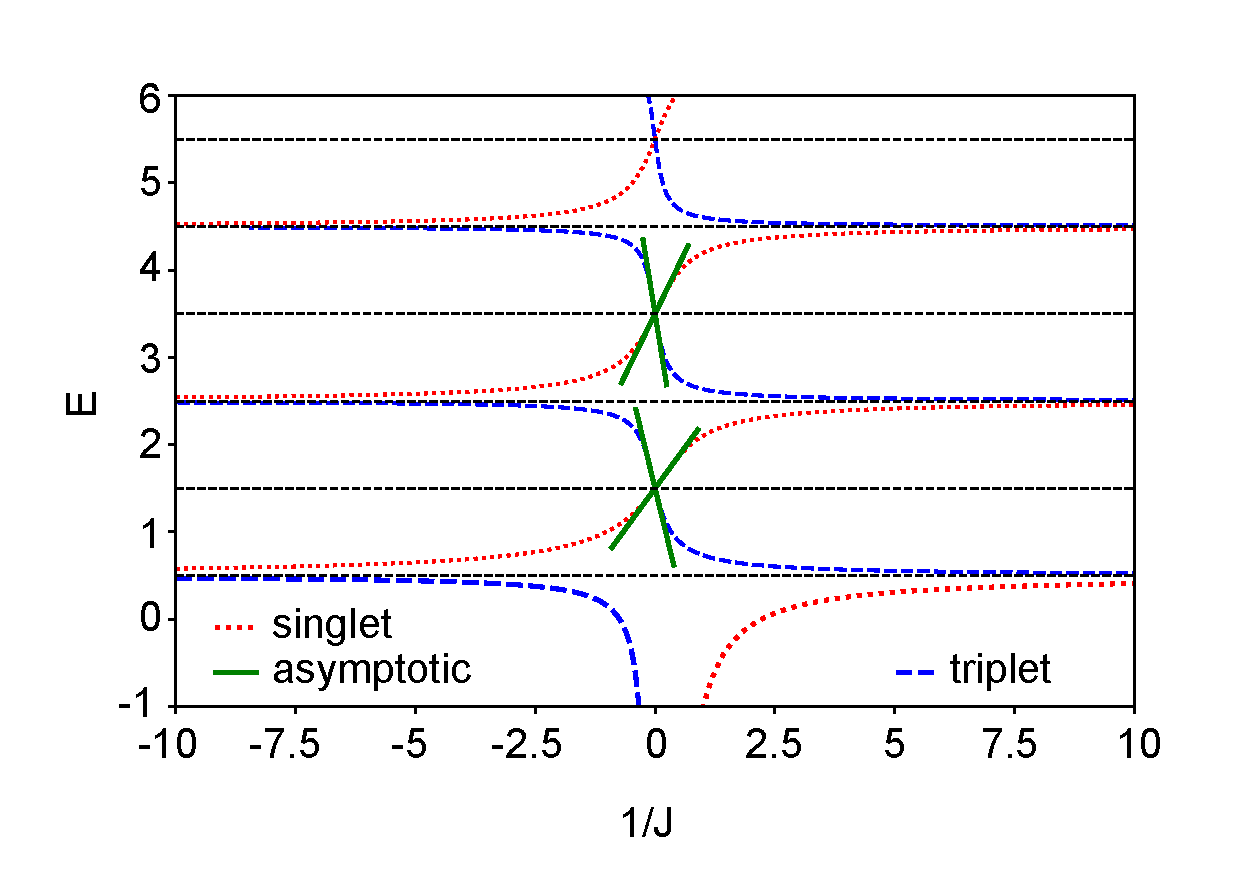
\includegraphics[width=0.7\textwidth]{fig1.pdf}
    \bicaption{一个杂质与一个费米子的1+1体系在$S_{tot,z}=0$子希尔伯特空间的能谱随自旋交换相互作用强度的变化。蓝色虚线(红色散点线)代表自旋三重态(自旋单重态)通道中的本征解。绿色实线代表强相互作用附近的微扰论渐近行为。其横纵坐标$E$与$J$的量纲为$\omega$与$\sqrt{\omega/M}$。}{(Color online). Energy spectrum of one fermion and one impurity in $S_{tot,z}=0$ subspace. The blue dashed (red dotted) lines show $E_t$ ($E_s$) for spin-triplet (singlet) eigen-states. The green solid line shows the asymptotic fitting to (\ref{asymptotic}) in strong coupling limit. Here the units of $E$ and $J$ are respectively $\omega$ and $\sqrt{\omega/M}$.}
    \label{fig:fig1}
\end{figure}

自旋交换部分已经被对角化,在各个通道内,自旋交换交换相互作用等价于纯的接触势,只不过接触势的符号受到自旋通道的影响。在如图~\ref{fig:fig1}~所示,我们展示了1+1两体中自旋单重态与自旋三重态通道的解,对应自洽方程(\ref{eq_t}与\ref{eq_s}),接下来我们来理解从这一能谱中得到的信息。



首先对于自旋单重态通道的解,对角化后的自旋交换相互作用对应强度为$\gamma_s=-3J/2$的接触相互作用,因此只有在$J>0$的时候,在散射态临界下面会有束缚态的产生。正如图~\ref{fig:fig1}~最下面的红色散点线所示,我们从$J=0$逐渐增大到$J=+\infty$,自旋单重束缚态的能量越来越低,在$J\to + \infty$附近,$E_s$渐近行为为$E_s\rightarrow -9J^2/8$。我们称这样的态为lower attractive branch。除了这支束缚态以外,我们发现其余的本征态在$J\to \pm \infty$的时候都趋近于有限大小的谐振子奇数能级,远远位于束缚态之上,我们称这样的一系列态为repulsive upper branch。如果我们逐渐放松谐振子的束缚程度,取$\omega\to 0$,我们会发现lower branch将变为一维接触势的唯一束缚态,而upper branch将变为一系列散射态。

对于自旋三重态通道的解,对角化后的自旋交换相互作用强度为$\gamma_t=J/2$,因此只有在$J<0$的时候才存在束缚态,如图~\ref{fig:fig1}~中最下面的蓝色虚线所示,当我们从$J=0$往负方向调节$J\to-\infty$时候,束缚态的能量不断降低,在$J\sim -\infty$附近其渐近行为是$E_t\rightarrow -J^2/8$。我们称这种态为lower attractive branch。类似地,在束缚态的上面,有一系列repulsive upper branch,它们的能量随$J\to-\infty$而趋近于谐振子的奇数能级处。

在$1/J=0$附近,我们看到不论单重态还是三重态的repulsive upper branch 能量都具有很好的线性行为,这表明此处可用微扰论来描述。具体地,我们以两体接触势$\gamma\delta(x)$为例(因为在三重态和多重态通道或中自旋交换相互作用被自动对角化为接触势),假设渐近行为是:
\begin{equation}
    E_m(\gamma) \simeq  (2m+1)\omega - \frac{A_m}{\gamma}.
\end{equation}
其中线性修正的系数$A_m$为待定。我们知道对于两体接触势来讲,势能部分哈密顿量带来波函数的边界条件,对任意$\gamma$:
\begin{equation}
    \gamma\psi_\gamma(0) = \frac{\psi'_\gamma(0)}{M}.
\end{equation}
根据Hellmann-Feynman定理,单参数哈密顿量能量对其参数的导数为:
\begin{equation}
\begin{split}
    \frac{dE(\gamma)}{d(1/J)} = -{}_\gamma\langle\psi| \gamma^2\delta(x) |\psi\rangle_\gamma
\end{split}
\end{equation}
其中$|\psi\rangle_\gamma$为接触势强度为$\gamma$时对应的某个本征解波函数,$E(\gamma)$为对应的本征能量,因此upper branch渐近行为的线性系数可由此计算:
\begin{equation}
\begin{split}
    A_m &= \lim_{\gamma\to \infty} -\frac{\partial E(\gamma)}{\partial \frac{1}{\gamma} }\\
    \quad &= \lim_{\gamma\to \infty} \int dx \gamma\psi_\gamma(x)\delta(x)\gamma\psi_\gamma(x) \\
    \quad &= \lim_{\gamma\to \infty} \gamma\psi_\gamma(0)\cdot \gamma\psi_\gamma(0). 
\end{split}
\end{equation}
最终我们得到单重态与三重态通道内upper branch的渐近行为:
\begin{equation}
E_{s/t,n} \simeq (2n+1)\omega -\frac{\phi^{'}_{2n+1}(0)^2}{M^2\gamma_{s/t}}. \label{asymptotic}
\end{equation}
其中$\phi'_n=d\phi_n(x)/dx$是谐振子本征波函数导数。在图~\ref{fig:fig1}~中,绿线代表了我们用此微扰论计算得到的线性行为,跟严格解的数值结果相一致。对应地,当$1/J=0$时候,系统的零阶未微扰波函数为\cite{zurn2012fermionization}:
\begin{equation}
|\Psi\rangle_{s/t,n} = \phi_{2n+1}(x) \cdot sgn(x)\left| s/t \right>, \label{asymptotic_wf}
\end{equation}
其中$|s\rangle = \frac{1}{\sqrt{2}}(|\uparrow\Downarrow - \downarrow\Uparrow\rangle)$,$|t\rangle = \frac{1}{\sqrt{2}}(|\uparrow\Downarrow + \downarrow\Uparrow\rangle)$ 具有自旋电荷分离的形式。
综上我们发现对于1+1体系,系统可以通过考虑各个通道中单粒子在接触势中的来图像方便地理解。最终的能谱也跟纯接触势中的1+1体系\cite{busch1998two}具有类似的行为。但是,随着我们在系统中再添加一个费米子,上面简单的单粒子图像便不再成立,能谱变得更加丰富,其中由自旋交换相互作用导致的新物理出现,这是完全不同于纯接触相互作用体系的新特性。在接下来的章节中们将对此详细介绍。

\subsection{一个杂质与两个费米子}

\begin{figure}[!htbp]
    \centering
    %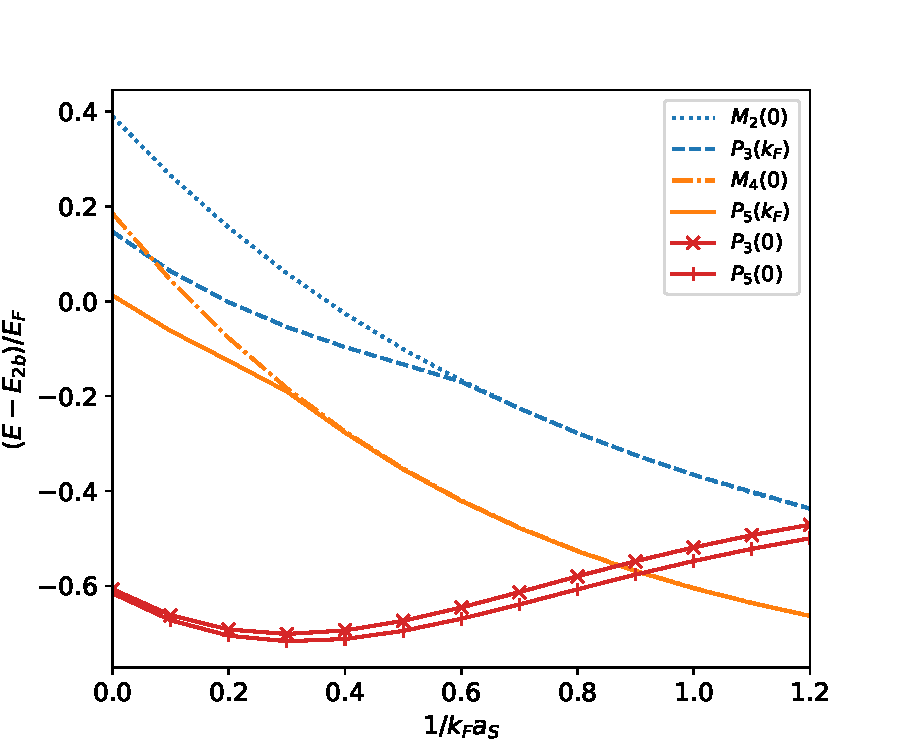
\includegraphics[width=0.7\textwidth]{fig2.pdf}
    \bicaption{一个杂质与两个个费米子的1+2体系在$S_{tot,z}=1/2$子希尔伯特空间的能谱随自旋交换相互作用与无自旋交换的接触相互作用强度的变化。a(1)代表的是带自旋交换相互作用1+2体系。我们用红色的点来标记其中特殊的$S_{tot=3/2}$的铁磁态。剩下的态都是$S_{tot}=1/2$的态。a(2)代表的是带纯接触势的1+2体系的能谱。其中$E$与$J$的量纲为$\omega$与$\sqrt{\omega/M}$。}{(Color online).(a1) Energy spectrum of two fermions and one impurity with spin-exchange interaction in the $S_{tot,z}=1/2$ subspace. The FM states with $S_{tot}=3/2$ are highlighted by red color, and the rest are all with total spin $S_{tot}=1/2$. (a2) Same as (a1) except that the interaction between fermions and impurity is a pure contact type without spin-exchange, see text. }
    \label{fig:fig2}
\end{figure}
根据前面章节讨论的一个杂质与两个费米子体系的变分求解,我们将关注点放在$S_{tot,z}=1/2$的封闭子希尔伯特空间中,图~\ref{fig:fig2}~展示了我们求解得到的三体能谱。可以清楚地看到,跟纯接触势的三体体系相比,带有自旋交换相互作用的三体体系能谱拥有更丰富的结构,接下来我们着重介绍由自旋交换相互作用带来的新奇特性。

首先,类似于1+1体系中attractive 与 repulsive branch的定义,我们将1+2体系里随着相互作用$|J|$从$0$到$\infty$,对应的本征能量趋近于$-\infty$的态称为attractive branch,将随着$|J|\to\infty$其本征能量趋近于有限数值的态称为upper branch。当然,这里的1+2体系都是处于谐振子势场中,如果取$\omega\to 0$,lower branch将过渡到一维少体束缚态(对于有限的$\omega$,当lower branch比较深的时候其行为已经非常接近一维接触势的束缚态了),upper branch将过渡到散射态。

具体地,图~\ref{fig:fig2}~a(1)中在铁磁($J<0$)与反铁磁($J>0$)两种情况下,我们注意到体系都有attractive branch,这是自然的。对应不同的磁性结构。作为对比,图~\ref{fig:fig2}~a(2)中展示的纯接触势的能谱则仅在$J<0$的情况下才有attractive branch。这是由自旋交换相互作用导致的最直接的能谱变化。进一步地,我们考虑强耦合极限下$|J|\to \infty$,lower branch的行为。

在铁磁耦合的情况下,随着$J\to+\infty$,我们发现,这些lower branch的渐近行为都是
\begin{equation}
E\sim\frac{-9J^2}{8}+C
\end{equation}
这个能量恰好是一个自旋单重束缚态的渐近行为。我们将$J>0$的能谱偏移$\frac{-9J^2}{8}$,结合我们对1+1体系的了解,图~\ref{fig:fig3}~a(1,2)中,我们看到减掉自旋单重态束缚能之后,剩余的能量趋近于$1.5\omega,3.5\omega...$。这些有限值远小于已经形成的自旋单重束缚态的能量。

鉴于能量上如此特殊的行为,我们得到物理图像上的启发,强铁磁耦合极限下,1+2体系中的两个费米子,其中一个被杂质束缚住,与杂质构成自旋单重束缚态,也可以说杂质自旋被其中一个费米子屏蔽。另一个费米子在已经形成的束缚态二聚体的影响下,只能形成repulsive branch,不能被进一步被二聚体所束缚,就好像这个可以束缚费米子的自旋被屏蔽了一样。从行为上很像掺杂金属中,局域杂质被费米面附近的电子所屏蔽,出现近藤单态类似\cite{mahanmany}。不过近藤屏蔽效应是一个典型的多体效应,不同于我们此处的少体物理,但是在我们的少体体系中,我们可以进一步添加巡游费米子来实现一个多体体系。随着添加费米子我们发现的这一图像还是否成立,以及与最终如何跟多体里面近藤屏蔽效应有何联系与区别,这些开放的问题都有待后续进一步的研究。

\begin{figure}[!htbp]
    \centering
    %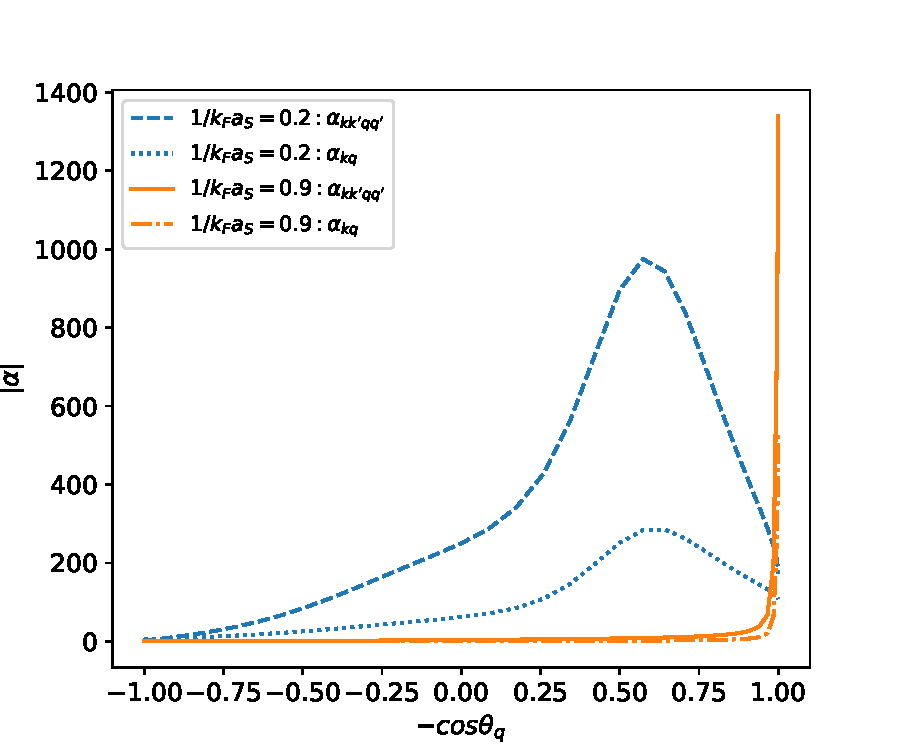
\includegraphics[width=0.7\textwidth]{fig3.pdf}
    \bicaption{铁磁($J>0$)与反铁磁($J<0$)耦合下整个体系平移对应的自旋单重态与自旋三重态能量后的能谱。其中a(1)代表能谱减掉$\frac{-9J^2}{8}$后的行为,b(1)代表了a(1)中灰色区域的放大。a(2)代表能谱减掉$\frac{-J^2}{8}$后的行为,可以看到基态依然随着$|J|$增大而能量越来越低,不再饱和到某一有限值。b(2)代表了a(2)中灰色区域的放大,从第一激发态开始,能量最终饱和在有限值。其中$E$与$J$的量纲为$\omega$与$\sqrt{\omega/M}$。}{a(1) Energies of deep bound states  for large and positive $J$, shifted by the spin-singlet binding energy $-9J^2/8$. All shifted energies saturate to a finite value, signifying the Kondo screening effect (see text).a(2) Energies of deep bound states  for large and negative $J$, shifted by the spin-triplet binding energy $-J^2/8$. The lowest bound state does not saturate as in b(1), showing the absence of screening effect for FM coupling. b(1,2) show the magnified plot for the shaded region in b(1,2), illustrating the asymptotic behavior towards odd harmonic levels. The units of $E$ and $J$ are respectively $\omega$ and $\sqrt{\omega/M}$.  }
    \label{fig:fig3}
\end{figure}

而在反铁磁情况下,基态branch的行为不同于铁磁情况。如图~\ref{fig:fig3}~a(2)所示,我们看到随着$J\to-\infty$,基态branch在减掉自旋三重束缚态二聚体能量$\frac{-J^2}{8}$之后依然越来越低,没有饱和在有限值。这表明此能量不仅由一个自旋三重束缚态贡献,剩下的那个费米子继续被二聚体所束缚,继续形成三体束缚态,导致能量进一步降低。除此之外,基态上面的激发态在减掉二聚体能量后最终趋向于有限的数值,如图~\ref{fig:fig3}~b(2)所示。

通过比较铁磁耦合与反铁磁耦合两种情况下基态的性质,我们发现对于一个杂质与两个费米子的1+2体系,铁磁耦合下,系统最多只能形成两体束缚态,局域的磁性杂质被一个费米子屏蔽之后无法再束缚更多的费米子。而对于反铁磁耦合,系统可以形成三体束缚态,局域杂质束缚了一个费米子之后还能继续束缚第二个费米子,导致能量比两体束缚态能量更低。这种特殊的少体关联效应是自旋交换相互作用所独有的。

为了进一步确认这种反铁磁耦合下系统的三体束缚态行为,我们考虑撤掉谐振子外势,考虑在一个一维自由体系,原点处固定一个自旋1/2的局域杂质,另有两个自旋1/2的全通费米子,长度为$L$,采用周期性边界条件,系统的哈密顿量为:
\begin{equation}
        \hat{H} = \sum_{j=1}^{2}  -\frac{1}{2M} \frac{\partial^2}{\partial x_{j}^2} + 2J\cdot\sum_{j=1}^2\delta(x_j){\hat{\Vector{S}}}_j\cdot {\hat{\Vector{S}}}.
\end{equation}
写在动量空间下的二次量子化哈密顿量为:
\begin{equation}\label{eq:free1+2}
\begin{split}
        \hat{H} &= \sum_{\Vector{k},\sigma}\epsilon_{\Vector{k},\sigma} \hat{C}^\dagger_{\Vector{k},\sigma} \hat{C}_{\Vector{k},\sigma}  + \sum_{\Vector{k}',\Vector{k}} \frac{J}{L} ( \hat{C}_{\Vector{k}'\uparrow}^\dagger  \hat{C}_{\Vector{k}\downarrow} \hat{S}_- + h.c. \\
        & \quad \quad +   (\hat{C}_{\Vector{k}'\uparrow}^\dagger  \hat{C}_{\Vector{k}\uparrow}-\hat{C}_{\Vector{k}'\downarrow}^\dagger  \hat{C}_{\Vector{k}\downarrow}) \hat{S}_{z} ).
\end{split}
\end{equation}
其中$\epsilon_{\Vector{k}} = \frac{\Vector{k}^2}{2M}$。在周期边界条件下,动量$\Vector{k} = \frac{2\pi\cdot n}{L}, n=0, \pm1, \pm2,...$。
在一维的情况下,对于纯接触势不需要做重整化,因此我们可以直接计算。由于方程(\ref{eq:free1+2})在形式上很类似于方程(\ref{eq:H2}),唯一的不同在于写在了不同的基矢表象下,对此我们依然采用矩阵对角化(\ref{final_eq})的办法,唯一的修改在于将其中的$\phi_m(0)$换为$\frac{1}{\sqrt{L}}$,$E_m$换为$\epsilon_{\Vector{k}}$,相应地,矩阵元变为:
\begin{equation}
\begin{split}
e_{kk'} &= \frac{1}{L}\frac{1}{E-E_k-E_{k'}}\\
q_{kk'} &= \delta_{kk'}  \frac{1}{L}\sum_p \frac{1}{E-E_k-E_p}\\
\end{split}
\end{equation}

在进行具体的数值计算之前,我们还需进一步讨论体系的特征尺度。在带有谐振子外势的体系中,系统有两个特征长度,分别是相互作用决定的$\frac{1}{MJ}$以及谐振子特征长度$\frac{1}{\sqrt{M\omega}}$。去掉谐振子之后的自由体系,仅有相互作用决定的特征长度$\frac{1}{MJ}$。因此我们用这个特征长度来做无量纲化,我们把具备这种特性的体系称为普适性体系。我们关心的物理是体系基态的束缚行为,对应的短程高能的物理,因此体系长度的选择于我们要考察的物理是不相关的,我们取足够大的动量截断$k_{\Lambda}/(MJ)=50$。{\color{red} 待补充 }

除了上面讨论的attractive branch的行为以外,我们还发现在能谱中有这样一类特殊的激发态。首先我们在能谱中将$S_{tot}=3/2$的态标记为红色。而且我们注意到这些$S_{tot}=3/2$的特殊态只在$J<0$的情况下成为lower attractive branch,在$J>0$的情况下趋向于有限值。如此特殊的行为也是很容易理解的,因为在$J>0$的区域,形成lower attractive branch的前提是其中一个费米子与杂质形成自旋单重二聚体束缚态,对应二聚体总的自旋为零,因此无法继续与剩下的费米子形成总自旋$S_{tot}=3/2$的自旋结构。由于自旋旋转对称性的保护,红色的$S_{tot}=3/2$与蓝色的$S_{tot}=1/2$的态之间永远正交,没有任何耦合,不会发生能级排斥现象。而且在$J>0$的情况下形成了upper repulsiev branch,我们称为铁磁repulsive branch。

如果我们仔细去考虑这支特殊的$S_tot=3/2$的铁磁branch的自旋部分,构型有三种:
\begin{equation}
    \begin{split} 
    |1\rangle &= |\uparrow\downarrow\Uparrow\rangle\\
    |2\rangle &= |\downarrow\uparrow\Uparrow\rangle\\
    |3\rangle &= |\uparrow\uparrow\Downarrow\rangle\\
    \end{split}
\end{equation} 
受到1+1中波函数自旋与空间分离的启发,其中铁磁要求任意一对自旋之间形成自旋三重态。我们构造$S_tot=3/2$的自旋波函数:
\begin{equation}
\Psi_{3,FM}(x_1,x_2)=\frac{1}{\sqrt{6}}\left|\begin{array}{cc}\psi_1(x_1) & \psi_1(x_2) \\\psi_2(x_1) & \psi_2(x_2)\end{array}\right| \left(|\uparrow\downarrow\Uparrow\rangle+|\downarrow\uparrow\Uparrow\rangle+|\uparrow\uparrow\Downarrow\rangle\right),
\end{equation}
其中自旋部分关于两个费米的自旋交换为对称,空间部分关于两个费米子交换为反对称。在这特殊的自旋构型下,相互作用中的自旋部分再一次地被对角化,自旋交换相互作用退化为纯的接触相互作用$U_t(x_i)=\gamma_t\delta(x_i)$,只影响波函数中的空间部分。其中$\psi_{1,2}$代表1+1体系中自旋三重态解的空间部分。我们巧妙的构造了这一特殊波函数,带入到薛定谔方程中:
\begin{equation}
\hat{H}\Psi_{3,FM}(x_1,x_2) = (E_1(J)+E_2(J))\Psi_{3,FM}(x_1,x_2)
\end{equation}
其中$E_1(J), E_2(J)$为1+1体系中自旋交换相互作用为$J$时候对应的自旋三重态本征能量。这时候三体体系是两体体系简单的相加。如果选取图~\ref{fig:fig2}~中三重态的基态与第一激发态,相加得到的三体能量即为铁磁态在整个相互作用区间的本征能量。$J\to-\infty$时,三体能量渐近行为是$E\to-\frac{J^2}{8}+1.5$;$J=0$时,$E=1.5+1.5=3$;$J\to\infty$时,$E\to1.5+3.5=5$。

值得一提的是,我们在自旋交换体系中发现的铁磁态与之前发现的自旋1/2费米子体系中的铁磁态\cite{cui2014ground}有很大不同,之前发现的铁磁态不会被s波相互作用所影响,其能量不随着相互作用变化。

除了上面讨论的铁磁态在$J>0$的时候是三体upper repulsive branch外,体系还有别的repulsive branch吗?要回答这个问题我们需要寻找能量随着相互作用$J\to\infty$而趋向于有限数值。我们仔细观察能谱,在能量$E=3\omega$附近有一支branch与能量不断降低的attractive branch发生能级排斥,$E=5\omega$附近有两条也发生能级排斥,发生能级排斥的位置最终逐渐饱和在有限值(随着$J\to\infty$能级排斥的能量区间越来越小,超过导致画图取点的分辨率),再加上已经发现的铁磁branch一共三条repulsive branch。受到铁磁态的启发,我们发现在$1/J=0$的极限情况下。铁磁的波函数为



\section{小结与展望}\label{sec:spex-summary}


%\chapter{极化子-分子转变的本质}\label{chap2polaron}

在论文的介绍部分{\color {red} 第一章}我们介绍了费米极化子的理论与实验研究脉络。其中三维和二维下极存在化子到分子的转变。一直以来这一转变的证据来自于两个分立的变分波函数。在我们最新的工作中,我们用一个截止到2对粒子-空穴对激发的统一变分波函数V-2ph来研究极化子-分子的转变。我们证实在三维和二维下确实存在极化子到分子的一阶转变。通过这一统一的变分波函数我们给出这一转变的本质在于不同总动量$\Vector{Q}=0$和$|\Vector{Q}|=k_F$和的转变。这里的$\Vector{Q}$指的是总动量相对于费米海的动量。之前研究中广泛使用的分子态变分波函数是我们V-2ph变分波函数$|\Vector{Q}|=k_F$在强相互作用下的渐近极限,并因此带来很大的$SO(3)$(三维是$SO(3)$,二维是$SO(2)$)基态简并。这一简并的发现导致了态密度的变化,这一变化改变了有限温度和有限密度下分子态的占据。我们与实验观测到的结果相比较,可以在弱耦合和共振区间得到较好的符合。我们进一步在二维下采用了高斯态的变分办法,验证了我们提出的极化子到分子的转变的本质在于动量的转变。在一维下变分法给出没有一阶转变,与贝特假设严格解的结果一致。最终得到极化子-分子的转变存在性由费米统计原理和维度带来的量子涨落共同决定。

\section{引言}
在论文的开始部分我们梳理了极化子理论与实验研究的进展。其中我们提到对于高维的情况,随着杂质原子与背景费米海之间相互作用的增强,系统基态发生极化子到分子的转变。相应的物理图像也很直观,当相互作用不那么强的时候杂质的运动被背景费米海的粒子空穴对激发所修饰,单粒子性质被重整化。一旦相互作用越过临界点,一个杂质可以与背景费米海的一个原子结合在一起形成服从玻色统计的分子态,不过这个分子态是有费米海存在的分子态,并不是真空的分子态。通常用两个独立的变分波函数来表征:
\begin{equation}
\begin{aligned}
&P_{2 n+1}(0) \\
&\quad=\left[\psi_{0} c_{\mathbf{0}_{\downarrow}}^{\dagger}+\sum_{l=1}^{n} \sum_{\mathbf{k}_{i} \mathbf{q}_{j}} \psi_{\mathbf{k}_{\mathbf{q}_{j}}} c_{\mathbf{P} \downarrow}^{\dagger} \prod_{i=1}^{l} c_{\mathbf{k}_{i} \uparrow}^{\dagger} \prod_{j=1}^{l} c_{\mathbf{q}_{j} \uparrow}\right]|\mathrm{FS}\rangle_{N}\\
M_{2 n+2}(0)=& {\left[\sum_{\mathbf{k}} \phi_{\mathbf{k}} c_{-\mathbf{k}, \downarrow}^{\dagger} c_{\mathbf{k}, \uparrow}^{\dagger}+\sum_{l=1}^{n} \sum_{\mathbf{k}_{i} \mathbf{q}_{j}} \phi_{\mathbf{k}_{i} \mathbf{q}_{j}} c_{\mathbf{P} \downarrow}^{\dagger}\right.} \\
&\left.\times \prod_{i=1}^{l+1} c_{\mathbf{k}_{i} \uparrow}^{\dagger} \prod_{i=1}^{l} c_{\mathbf{q}_{j} \uparrow}\right]|\mathrm{FS}\rangle_{N-1}
\end{aligned}
\end{equation}
这里$\hat{c}^\dagger_{\Vector{k},\sigma}$为动量为$\Vector{k}$的自旋$1/2$费米子。在我们接下来中取自旋向上为背景原子,$|FS\range_N$为N个原子的费米海。自旋向下为杂质原子。求和中的$\Vector{q}$限制在费米球内部,$\Vector{k}$限制在费米海外部。其中$\Vector{P}=\sum_{j} \Vector{q}_{j}-\sum_{i} \Vector{k}_{i}$,通过分别将变分波函数带入到薛定谔方程中可以得到极化子分子一阶转变的图像。尽管这种分立的变分波函数物理上很直观,但是这种两个预先选定的变分波函数来给出相变带有很大的认为选择因素。对此最直接的一个不完善点在于一个观察\cite{edwards2013smooth}:该研究发现以上两个变分波函数通过考虑不同的角动量和不同阶的粒子空穴对激发下是互相包含的。因此在这个意义下,这种分立的变分波函数需要小心对待。

而在实验这边,实验解析到的准粒子留数是连续地趋向于零,并没有出现跳变。尤其是最近的实验通过动量分辨的Raman谱直接解析到不同物理量在转变前后连续的变化\cite{Sagi2020}。再一次印证了变分波函数下极化子到分子的转变需要谨慎对待。

基于上面理论与实验方面的动机,在最近的研究中,通过统一的变分波函数来研究极化子与分子的必要性被重视起来\cite{Cui2020Fermi}。通过统一的变分波函数$V-1ph$:$P_3(\Vector{Q}),即将动量扩展到非零动量$来研究三维极化子。我们这里的$\Vector{Q}$指的是系统总的动量减掉费米海$|FS\range_N$的动量。

\section{模型}

\section{结果}

\section{小结与展望}


\chapter{热化中的反常动力学}\label{chap:ETH}

孤立系统的热化在理解宏观系统的量子统计描述中扮演重要的角色。对于仅有局域相互作用的哈密顿量,本征热化假说被提出用来给出孤立系统热化的解释。目前为止对此假说的论证主要集中于数值模拟。但是人们目前还不严格清楚其适用的范围。有趣的的是在一些特殊体系中,本征热化假说完全失效,称为强违背本征热化假说体系,其中以量子可积系统与多体局域化系统最为典型。随着认识的不断加强,依赖于初态选取的弱违背本征热化假说体系被发现:从某些初态出发会热化,但是从某些初态出发则不会热化。在本章中,我们选择固定的初态如$|Z_2\rangle$出发,探索整个参数区间下带有纵场的横场伊辛模型的热化相图,并讨论发现的不同热化区域及其背后的物理解释。我们在~\ref{4sec:intro}~节中给出此研究的动机,~\ref{4sec:method}~节中讨论涉及的模型和方法,~\ref{4sec:result}~节中针对得到的热化相图做分析,我们主要发现了整个many body scar区域的非热化行为,并于严格可解极限做了联系,最后我们还发现了基态附近的弱热化行为。在~\ref{4sec:sum}~节我们总结目前的结果并做简要的小结。

\section{引言}\label{4sec:intro}
在热力学平衡态的角度,量子统计力学给出了宏观物体的热力学描述。仅用几个参数就可以描述处于热力学平衡态的宏观数目自由度的体系。而量子统计力学中一个关键原理即是等概率原理——具有相同能量的微观量子态在热力学平衡态分布中出现的几率相同。基于此原理,我们引入微正则系综来描述平衡态分布,为了与实验体系方便比较,我们又引入了在热力学极限下与之等价的正则系综与巨正则系综。但是在另一个角度,根据量子力学基本定律,我们知道孤立量子体系的演化为幺正的。如果我们准备一个孤立系统处于初态$|\psi(t=0)\rangle$,初态在不同本征态上的投影几率为$\langle E_\alpha|\psi(t=0)\rangle$,这一几率在幺正时间演化下是不变的。对于一个系统的长时间平均测量,其观测值似乎在初态决定的时候就已经决定了,看似是初态依赖的,这与统计力学中假设的时间平均等价于等概率系综平均乍一看是矛盾的。为了解决这一矛盾,Deutsch J M\cite{Deutsch1991quantum}与Srednicki M\cite{Srednicki1994chaos}分别独立地提出了本征热化假说(ETH),其核心思想为当我们观测一个孤立系统的局域可观测量时,系统的剩余部分作为这个局域自由度的热库,这一热接触的温度由系统总的能量给出。这一假说在后续很多体系的数值试验中得到验证。具有很强的普适性,局域算符的可观测量仅由能量决定。更加形式化的讨论以及数值证据可以参见我们~\ref{1sec:ETH}~节中给出的介绍。但大自然总是奇妙的,这一假说很快就被发现在某些体系里面完全失效,其中以量子可积系统\cite{kinoshita2006quantum,Rigol2007Relaxation,Calabrese2011Quantum,essler2016quench,vidmar2016generalized}与多体局域化系统最为典型\cite{basko2006metal,Serbyn2013local,Huse2014Phenomenology},其完全失效的原因目前仍没有确切定论,这种体系被称为完全违背本征热化假说体系。

完全符合本征热化假说与完全违背本征热化假说是两个极端。很快介于两个极端的弱违背本征热化假说系统被发现。典型的例子就是量子多体伤痕。这一现象最早发现于冷原子中里德堡原子平台\cite{bernien2017probing}。在一维原子链中,每个格点上里德堡原子近似为二能级体系,原子间的库伦相互作用禁止相邻的两个原子处于二能级中的里德堡激发态,可以用PXP哈密顿量来描述。该实验在$|Z_2\rangle$初态出发的动力学中发现了局域算符反常的长时间震荡行为,并且其时间平均值并不等于吉布斯系综所预测的热力学吉布斯正则系综平均值。
这一实验很快地激发了相关的理论研究\cite{turner2018weak,Turner2018quantum,Ho2019periodic,Choi2019emergent,Michailidis2020slow,serbyn2021quantum,Yao2022quantum},这一反常动力学来自于PXP哈密顿量中涌现出的近似封闭的子希尔伯特空间。数值严格对角化的结果给出这一子空间里的本征态违背本征热化假说的规律。而不在此子空间的态则服从本征热化假说。基于这一图像,严格封闭的子希尔伯特空间在不同哈密顿量中被构造出来\cite{Shiraishi2017Systematic,Moudgalya2018exact,Moudgalya2018entanglement,Khemani2020lacalization,Moudgalya2020eta,Lin2019Exact,Schecter2019weak,Mark2020unified,Mark2020eta,Pakrouski2020many,Ren2021quasi,ODea2020from},自然地这些空间里的态也违背本征热化假说。但是这些态为何存在?如何在一个哈密顿量中找到这些态?我们离这些问题的答案依然很遥远。除了量子多体伤痕,在一些格点规范模型\cite{magnifico2020real,Chanda2020confinement,Borla2020confined}和禁闭模型\cite{Nandkishore2017many,kormos2017real,Robinson2019signature,Yang2020Hilbert,Castro2020entanglement}中也有观测到这种弱本征热化假说违背的现象。其与量子多体伤痕的关系目前仍尚未明确\cite{serbyn2021quantum}。


介于完全服从本征热化假说与完全违背本征热化假说的中间情况还有一种叫做弱热化的现象\cite{banuls2011strong}。这是在带有纵场的横场伊辛模型中被发现的。当纵场不为零时候,该模型不再是可积的。通常来讲没有无序的不可积模型是热化的,会符合本征热化假说。但是张量网络模拟的结果给出,从$|Z+\rangle$出发的动力学表现出一种围绕热力学均值震荡的行为。这一震荡并不是热力学涨落,被称为弱热化现象。这一现象的一个解释是震荡由基态附近准粒子激发带来\cite{Lin2017quasiparticle}。并且这一反常行为在超导量子比特模拟中被发现\cite{Chen2021observation}。

基于上述的讨论,我们看到各种热化与非热化的现象。对于一个哈密顿量来讲,本征热化假设总归是一个很严格的要求,很容易有部分违背这一假说本征态。简单的做二分类是粗糙的。目前的研究很多是固定莫某个参数或者选取某个初态来研究。在我们本章工作中,我们基于带有纵场的横场伊辛模型,选取固定的基态$|Z_2\rangle$出发,在整个带有纵场的横场伊辛模型参数区间研究其热化的相图,以期得到一个较为全面的认识。

\section{模型与方法}\label{4sec:method}
我们采用严格对角化的数值方法来研究带有纵场的横场伊辛模型,我们取$g=1,\hbar=1$,哈密顿量为。
\begin{equation}
\hat{H}_{Ising} = J\sum_{i}\hat{\sigma}^z_i\sigma^z_{i+1} + h\sum_{i}\hat{\sigma}^z_i + g\sum_i\hat{\sigma}^x_i
\label{Ising}
\end{equation}
选取周期性边界条件,选取$|\downarrow\rangle=|0\rangle$,$|\uparrow\rangle=|1\rangle$,其中$\sigma_i^{x,y,z}$为泡利算符。

\subsection{对称性}
哈密顿量拥有晶格平移对称性以及空间反演对称性。对于晶格平移对称性,我们定义平移算符$\hat{T}$:
\begin{equation}
	\hat{T} |0,1 \rangle_{i} =  |0,1 \rangle_{i+1}, i=1,2...L
\end{equation}
平移算符与哈密顿量对易:
\begin{equation}
	\hat{T}^{-1}\hat{H}_{Ising}\hat{T} = \hat{H}_{Ising}\\
\end{equation}
因此我们选取布洛赫动量态,作为晶格平移算符与哈密顿量共同本征态。布洛赫动量量子数可以取 $K_i=\frac{2\pi\cdot i}{L},i=0,1...L-1$,为动量算符$\hat{K}$的本征值,其中$\hat{K}$的定义为$\hat{T} = e^{-i\cdot\hat{\vec{K} }\cdot \vec{a}}$的生成元。

第二个全局对称性为空间反演对称性$\hat{I}$:
\begin{equation}
	\hat{I} |0,1 \rangle_{i} =  |0,1 \rangle_{L+1-i}, i=1,2...L
\end{equation}
同样地与哈密顿量对易关系为:
\begin{equation}
	\hat{I}^{-1}\hat{H}_{Ising}\hat{I} = \hat{H}_{Ising}\\
\end{equation}

不巧的是$\hat{K}$ 与 $\hat{I}$并不对易。但是在某些动量态比如$K_i=0$ 与 $K_i=\pi$子空间中,反演算符与$\hat{K}$与$\hat{I}$是对易的,此时我们可以进一步将空间划分为宇称为$+$与$-$的子空间。
\begin{comment}
在做了如上所述的块对角化之后,我们将要严格对角化的矩阵维度最大为动量宇称$KP=0+$
子空间的维度$L=18,KP=0+$,此时$D=7685$。
\end{comment}

\subsection{时间平均与系综平均}
考虑某个初态出发,在判断系统的局域可观测量最终是否热化时,我们需要将长时间平均的结果与热力学吉布斯系综平均的结果做比较。其中对于时间平均,在将对称性导致的简并考虑完毕后,体系通常情况下不再拥有简并。我们记此时子空间的本征能量与本征解为$E_\alpha$ 与 $|\alpha\rangle$:
\begin{equation}
\hat{H} |\alpha\rangle = E_\alpha |\alpha\rangle, \alpha=1,2...D
\end{equation}
其中D为考虑全局对称性块对角化之后子空间的维度。当考虑局域算符$\hat{L}$的长时间演化时,从初态$|\psi(t=0)\rangle$出发,t时刻$|\psi(t)\rangle$ 有:
\begin{equation}
|\psi(t)\rangle = e^{-i\hat{H}t}|\psi(t=0)\rangle = \sum_{\alpha=1}^D e^{-i E_\alpha t} \langle\alpha|\psi(t=0) \rangle  |\alpha\rangle
\end{equation}
时间平均为:
\begin{equation}
\begin{split}
	\bar{L}_{\infty}  &= \lim_{T\to \infty} \frac{1}{T} \int_{t_0}^{t_0+T} \langle\psi(t)|\hat{L}|\psi(t)\rangle dt \\
		\quad &=  \sum_{\alpha} \langle\alpha|\hat{L}|\alpha\rangle |\langle\alpha|\psi(t=0)\rangle|^2  +  \lim_{T\to \infty} \frac{1}{T} \int_{t_0}^{t_0+T} dt \\
		&\quad \cdot\sum_{\alpha\neq\gamma} \langle\alpha|\hat{L}|\gamma\rangle \langle\gamma|\psi(0)\rangle \langle\psi(0)|\alpha\rangle e^{-i(E_\gamma-E_\alpha)t}
\end{split}
\end{equation}
从黎曼积分定理我们知道非对角元的部分在长时间$T\to\infty$平均下贡献为零。仅剩对角元部分有贡献,此即对角系综:
\begin{equation}
	\bar{L}_{\infty} =  \sum_{\alpha} \langle\alpha|\hat{L}|\alpha\rangle |\langle\alpha|\psi(t=0)\rangle|^2  = Tr(\hat{\rho}_{DE}\hat{L}) = \bar{L}_{DE}
\end{equation}

而在另一方面,考虑吉布斯系综平均时我们有平均能量与动量定义为:
\begin{equation}
\begin{split}
 \bar{E} &= \langle\psi(t=0)|\hat{H}|\psi(t=0)\rangle \\
 \bar{K} &= \langle\psi(t=0)|\hat{K}|\psi(t=0)\rangle\\
\end{split}
\end{equation}
接着我们定义对应吉布斯系综分布:
\begin{equation}
\hat{\rho}_{th} = \frac{1}{Z}e^{-\beta\hat{H}-\lambda\hat{K}}, Z = Tr(e^{-\beta\hat{H}-\lambda\hat{K}})
\end{equation}
其中的$\beta,\lambda$由下式给定:
\begin{equation}
\begin{split}
	\bar{E} &= Tr(\hat{\rho}_{th}\hat{H} ) \\
	\bar{K} &= Tr(\hat{\rho}_{th}\hat{K})
\end{split}
\end{equation}
一旦我们得到$\beta$ 与 $\lambda$,局域算符的热力学系综期望值即为:
\begin{equation}
	\bar{L}_{th} = Tr(\hat{\rho}_{th}\hat{L})
\end{equation}

为了消除严格对角化中尺寸的效应,我们对两种平均都做了有限尺寸修正。

\section{相图与分析}\label{4sec:result}
我们主要的数值模拟结果可以总结在下面的相图里面,对于固定的哈密顿量,参数为$J,h$,我们从初态$|Z_2\rangle$出发,我们考虑局域算符$\hat{L}=\hat{\sigma}_1^z\hat{\sigma}_2^z$,比对由对角系综求得的长时间平均以及正则系综平均得到吉布斯平均,比较两者之间的差值,我们画出有限尺寸修正后的结果:

%***********************************
\begin{figure}[h]
\centering
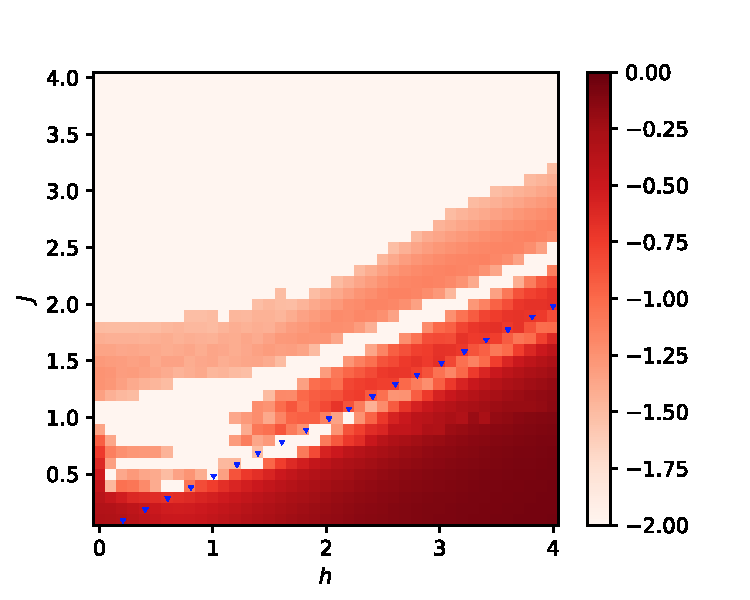
\includegraphics[width=0.7\textwidth]{./scar/scar1.pdf}
\bicaption{初态为$|Z_2\rangle$的局域算符时间平均期望值与吉布斯系综平均期望值之差。选取不同的链长L=10,12,14,16,18,我们做有限尺寸修正,然后对两种平均的期望值做差取绝对值后再画在10为底的对数坐标下。我们选取截断$\Delta=0.03$作为临界值,绝对值低于临界值的我们在图中用白色表示。绿色的点标记$J=\frac{h}{2}$。}{Difference between long time average and Gibbs canonical ensemble average of local operator $\hat{L}=\hat{\sigma}_1^z\hat{\sigma}_2^z$. By choosing different length of chain $L=10, 12,14,16,18$, we do finite size scaling to obtain $L=\infty$ result and take $log_{10}$ for difference. We choose critical difference between two average to be $\Delta=0.03$. When $|\Delta|<0.03$, we mark as white color to represent thermalization. Green points mark special line $J=\frac{h}{2}$. }
\label{scarphasediag}
\end{figure}
%***********************************

我们将相图分为几个区域来讨论:


\subsection{Many body scar区域}
首先是many body scar区域,对于里德堡哈密顿量,带入$\hat{n}_i = \frac{\hat{\sigma}_i^z+1}{2}$:
\begin{equation}
\begin{split}
	\hat{H}_{Rydberg}(V) &= \sum_{i=1}^{L} \hat{\sigma}_{i}^{x} + V \sum_{i}^{L} \hat{n}_i\cdot\hat{n}_{i+1} \\
	\quad &= \sum_{i=1}^{L} \hat{\sigma}_{i}^{x} + \frac{V}{4}  \sum_{i}^L \hat{\sigma}_i^z\hat{\sigma}_{i+1}^z + \frac{V}{2} \sum_i^L \hat{\sigma}_i^z  + \frac{V}{4} \sum_i^L \hat{1} \\
\end{split}
\end{equation}
我们发现如果在$\hat{H}_{Ising}(g,J,h)$中取$g=1,J=V/4,h=V/2$,则两者是等价的(仅相差一个与链长有关的常数):
\begin{equation}
\hat{H}_{Ising}(g=1,J=\frac{V}{4},h=\frac{V}{2}) = \hat{H}_{Rydberg}(V) + C
\end{equation}
因此在带有纵场的横场伊辛模型中,如果沿着$J=h/2$这条特殊的线来看,在$J$较大的极限下,有效模型为PXP模型,。

如果我们把$J=h/2$这条线从相图里摘出,我们就得到了里德堡哈密顿量,对应$V=4J$,如图~\ref{scar1_2}~(a)所示。沿着$J=h/2$这条线,当$J\ll 1$处于弱耦合的时候,此时由于靠近单自旋极限,从$|Z_2\rangle$出发的动力学具有非热化的行为是可以期待的。当$J\gg 1$处于强耦合的时候,此时为PXP极限,基态子空间对应没有近邻格点同时处于$\uparrow$,有效模型为:
\begin{equation}
	\hat{H}_{PXP} = \sum_i\hat{P}_{i-1}\hat{\sigma}_{i}^x\hat{P}_{i+1}
\end{equation}
其中$\hat{P}_i=|\downarrow\rangle\langle\downarrow|$,从$|Z_2\rangle$作为初态出发,会观察到局域算符期望值的持续震荡行为,其长时间系综平均不等于热力学系综平均,此即量子多体伤痕动力学。这是违背本征热化假说的反常动力学。在中间区域$h\sim 1$,我们看到由于时间平均随着$J$的变化存在一极大值结构,导致仅在与热力学吉布斯正则系综平均曲线的两个交点处有局域算符的时间平均与系综平均之差为0,在其余情况下局域算符期望的时间平均不等于系综平均。随着$J$从0开始增大,体系逐渐远离单自旋极限,同时局域算符的时间平均与热力学系综平均的差值在缩小,但是随着$V=4J$慢慢增大,PXP有效模型开始涌现,再一次使得局域算符的时间平均期望值远离了其热力学系综平均期望值。对于这一连续的渡的过程,我们展示更多的细节我们分别取三个不同的参数区间下计算与本征态与初态的投影、半链纠缠熵与实际动力学,如图~\ref{scar1_2_detail}~所示:
%***********************************
\begin{figure}[h]
\centering
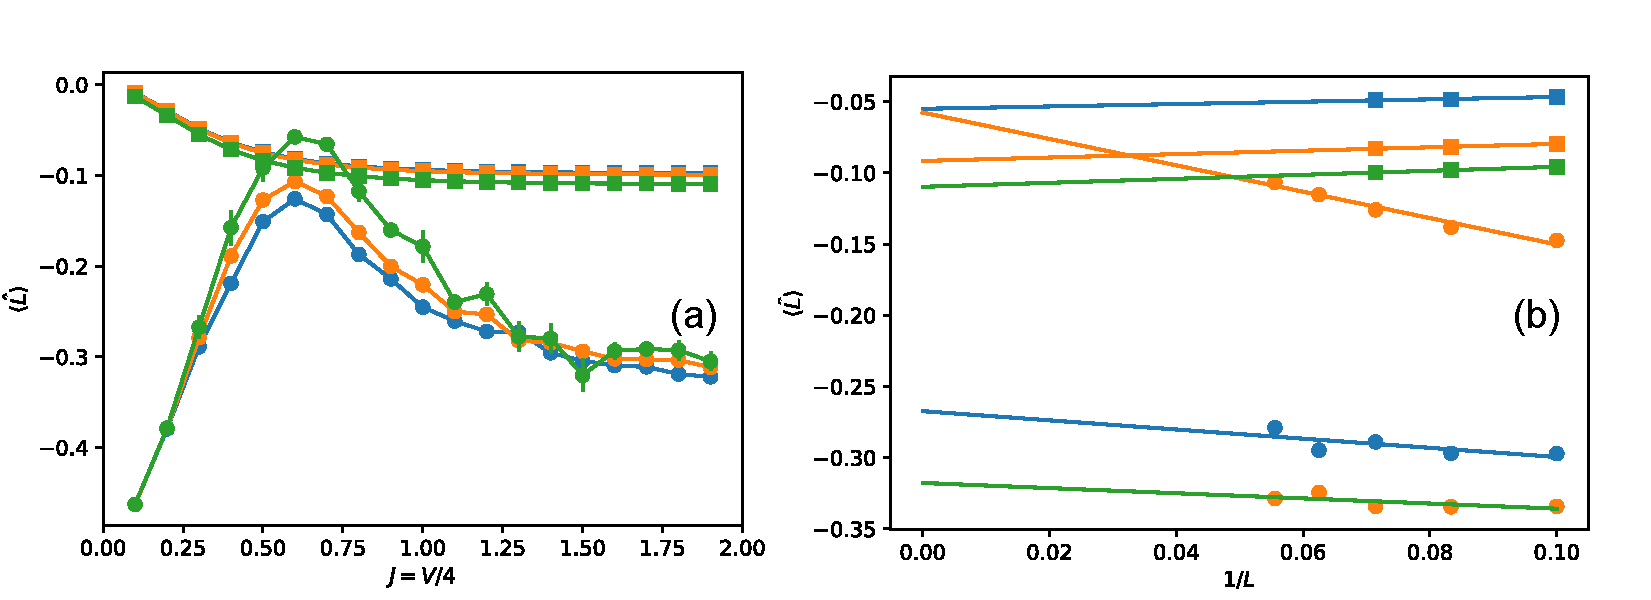
\includegraphics[width=0.9\textwidth]{./scar/scar2.pdf}
\bicaption{图(a)为沿$J=h/2$特殊比例下局域算符$\hat{L}=\hat{\sigma}_1^z\hat{\sigma}_2^z$时间平均(圆点)与系综平均(方点),其中蓝色点为$L=14$,橘色点为$L=18$,绿色点为有限尺寸修正结果,带有线性拟合的误差。图(b)为$J=0.3$(蓝色),$J=0.6$(橘色),$J=2.5$(绿色)下的有限尺寸修正,圆点代表时间平均,方点代表吉布斯系综平均。}{ Fig (a) for time average(dots) and Gibbs canonical ensemble average(square points) of local operator $\hat{L}=\hat{\sigma}_1^z\hat{\sigma}_2^z$ along $J=h/2$, blue points for $L=14$, orange points for $L=18$ and green points for result of finite size scaling with error bar of linear fitting. Fig (b) for finite size scaling of time average(dots), Gibbs conanical ensemble average(square points) and linear scaling fitting (solid lines) under $J=0.3$(blue), $J=0.6$(orange), $J=2.5$(green). }
\label{scar1_2}
\end{figure}
%***********************************
从图(a,b)中我们可以看到,在弱耦合以及中间区域,与初态$|Z_2\rangle$交叠较大的本征态中,都会有一些反常低熵态。此时能谱尚未在里德堡库伦blockade的作用下发生片段化(以相邻的$\uparrow\uparrow$的数目来分隔不同的片段),这些反常低熵态处于能谱中靠近基态的位置,正是由于这些反常低熵态的存在导致这一非热化行为的出现,其动力学如图(d,e)所示。在图(c,f)中我们进一步展示了PXP极限下的情况,在这一极限下这些由于能谱发生片段化,仅考虑最低子空间中(没有$\uparrow\uparrow$),与初态$|Z_2\rangle$交叠较大的本征态中仍然会出现反常低熵态,这些反常低熵态有规律的近似等间距分布,导致局域算符动力学中具有清晰的非热化震荡行为。
%***********************************
\begin{figure}[h]
\centering
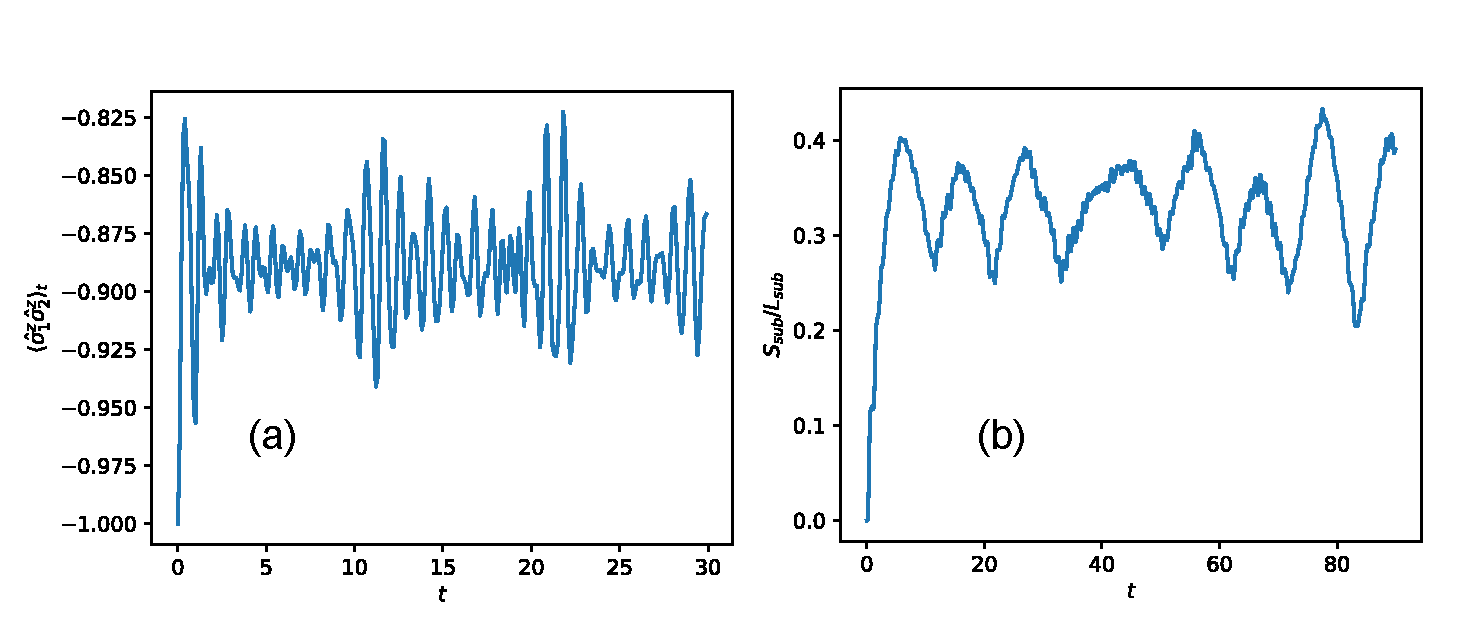
\includegraphics[width=1.2\textwidth]{./scar/scar3.pdf}
\bicaption{不同参数$J$下的本征态到初态投影权重、半链纠缠熵、演化动力学。其中(a,d)对应$J=0.3$,(b,e)对应$J=0.6$,(c,f)对应$J=2.5$。图(a,b,c)中散点代表与初态的投影权重,颜色代表半链纠缠熵。图(d,e,f)代表不同$J$下从初态为$|Z_2\rangle$出发的局域算符动力学。橘黄色虚线代表有限尺寸修正后$\hat{L}$的热力学吉布斯正则系综平均。}{Overlap between initail state and eigenstate, entanglement entropy of half chain and local operator dynamics under different J: (a, d)$J=0.3$, (b, e) for $J=0.6$, (c, f) for $J=2.5$. In Fig (a, b, c) scatterd dots for overlap and color bar for entanglement entropy of half chain. Fig (d, e, f) for dynamics of $\hat{L}=\hat{\sigma}_1^z\hat{\sigma}_2^z$ under different J starting from $|Z_2\rangle$. Orange dashed lines for Gibbs conanical ensemble average of $\hat{L}$ after finite size scaling.}
\label{scar1_2_detail}
\end{figure}
%***********************************

%***********************************
\begin{figure}[h]
\centering
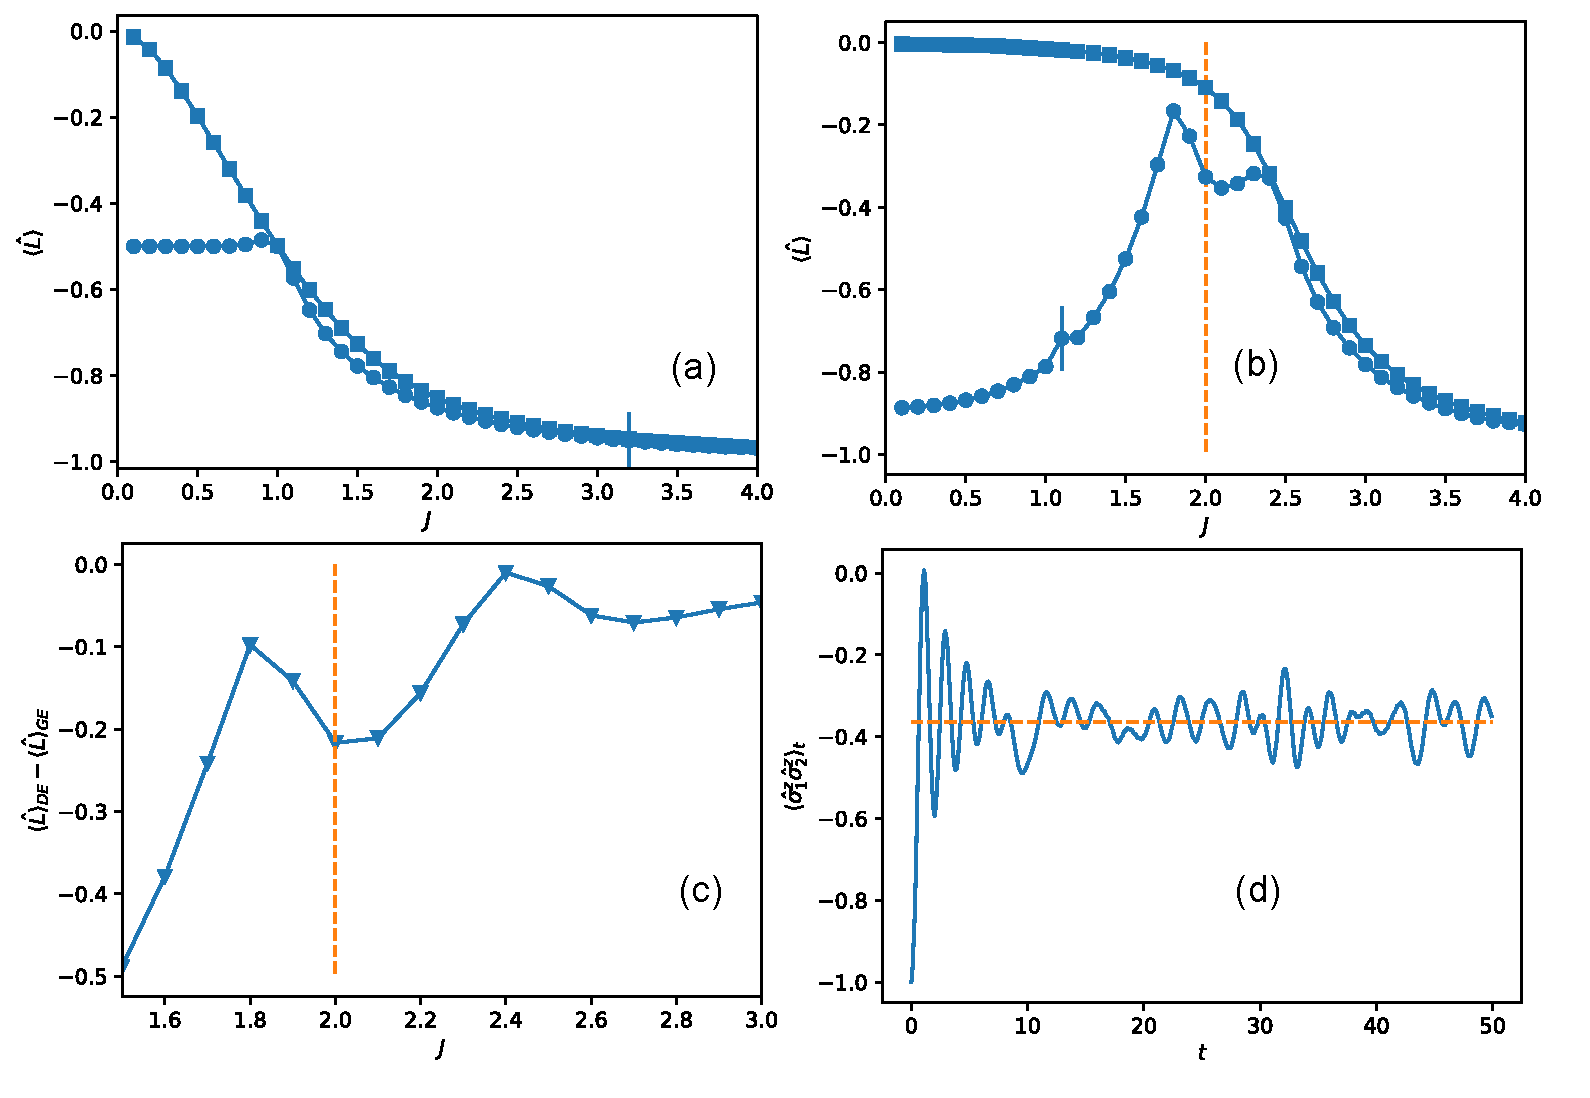
\includegraphics[width=0.8\textwidth]{./scar/scar4.pdf}
\bicaption{图(a)为$h=0$下$\hat{L}=\hat{\sigma}_1^z\hat{\sigma}_2^z$的时间平均与热力学吉布斯正则系综平均。图(b)为$h=4$下的时间平均与热力学吉布斯正则系综平均。圆点代表有限尺寸修正下的时间平均,方点代表有限尺寸修正下的热力学吉布斯正则系综平均。图(c)三角点为沿$h=4$局域算符$\hat{L}$的有限尺寸修正后时间平均与吉布斯系综平均的差值。图(b,c)中橘黄色虚线代表$J=h/2$处。图(d)为$L=16,J=2.4,h=4$下的局域算符期望值动力学演化。图(d)中橘黄色虚线代表有限尺寸修正后的热力学吉布斯正则系综平均。}{  Fig (a, b) for time average and Gibbs canonical ensemble average of local operator $\hat{L}=\hat{\sigma}_1^z\hat{\sigma}_2^z$ under $h=0$(a) and $h=4$(b). Dots for time average and square points with error bar for Gibbs canonical ensemble average after finite size scaling. In Fig (c) triangle ponits for difference between time average and Gibbs canonical ensemble average. Orange dashed line in Fig (b, c) for $J=h/2$. Fig (d) for dynamics of local operator $\hat{L}=\hat{\sigma}_1^z\hat{\sigma}_2^z$ starting from $|Z_2\rangle$ under $J=2.4,h=4$. Orange dashed line in Fig (d) for Gibbs canonical ensemble average of local operator after finite size scaling. }
\label{h04}
\end{figure}
%***********************************
在上述沿着$J=h/2$的特殊比例下,我们分析了相图的热化性质。进一步我们在PXP极限下,改变这一$h:J$的比例,探索不同$J$带来的影响,此时我们选取足够大的$h=2$,对于$J=h/2+a$,则在$h,J\gg a$的区域:
\begin{equation}
\begin{split}
\hat{H}_{Ising}&=\sum_i\hat{\sigma}^x_i + J\sum_{i}\hat{\sigma}^z_i\sigma^z_{i+1} + 2(J-a)\sum_{i}\hat{\sigma}^z_i  \\
\quad &= \sum_i\hat{\sigma}^x_i + 4J\sum_{i}^{L} \hat{n}_i\cdot\hat{n}_{i+1} - 2a\sum_{i}\hat{\sigma}^z_i  + C\\
\end{split}
\end{equation}
额外纵场项会变成PXP模型中的$h_{eff}\sum_i\sigma^z_i = -2a\sum_i\sigma^z_i$,物理意义相当于在PXP模型中再加一个沿$z$方向纵场,即:
\begin{equation}
\hat{H}_{eff} = \sum_{i}^{L} \hat{P}_{i-1}\hat{\sigma}_i^x\hat{P}_{i+1} + h_{eff}\sum_i\hat{\sigma}^z_i 
\end{equation}
在图~\ref{h04}~(b)中我们给出这一PXP极限附近加有效磁场的时间平均与热力学吉布斯正则系综平均,在图~\ref{h04}~(c)中我们给出两种平均的差值。随着a的增大,$h_{eff}<0$,首先会破坏many body scar动力学,使其先变为热化的行为,大约在$a_c=0.4$附近,此时多体伤痕动力学被完全破坏,此时动力学如图~\ref{h04}~(d)所示,这一现象在最近的研究中已经被发现\cite{Yao2022quantum}。如果反向增加磁场及$h_{eff}>0$,我们也会看到这一非单调的行为,表明many body scar动力学反常行为被抑制,但是并没有被彻底破坏,如图~\ref{h04}~(c)所示。

而在$h=0$时,此时为严格可解的横场伊辛模型,此时我们展示这一严格可解系统的时间平均与热力学系综平均,如图~\ref{h04}~(a)所示。可以看到仅在$J=1$时间平均等于系综平均,对于这样的严格可解模型,研究者提出用generalized Gibbs ensemble可以给出整个$J$区间的广义热化预测\cite{vidmar2016generalized}。而在$J\gg 1$极限下,系统进入特殊的弱热化区间。



\subsection{弱热化区域}
在相图的上半部分,此时$J \gg \frac{h}{2}$,当$g=0$时,我们有$|Z_2\rangle=|10101010...\rangle$与$|Z'_{2}\rangle=|0101001...\rangle$为系统的两个简并基态。但是着两个简并基态无法通过动力学联系起来。当$g\neq 0$时候,打开量子涨落,动力学局限在基态以及基态附近的准粒子激发附近。此时的准粒子激发主要有两类,近似为$|...00...\rangle$
与$|...11...\rangle$,对应的准粒子能量为$4J-2h$与$4J+2h$,当初态处于$|Z_2\rangle$时,此时的动力学即由准粒子决定的弱热化动力学。其震荡频率反映的是准粒子的能量,其振幅由$\sum_i \hat{\sigma}_i^x$引发的量子跃迁决定,如图~\ref{weak}~所示,同时单自旋的熵远低于$ln2$并伴有明显的震荡行为。
%***********************************
\begin{figure}[h]
\centering
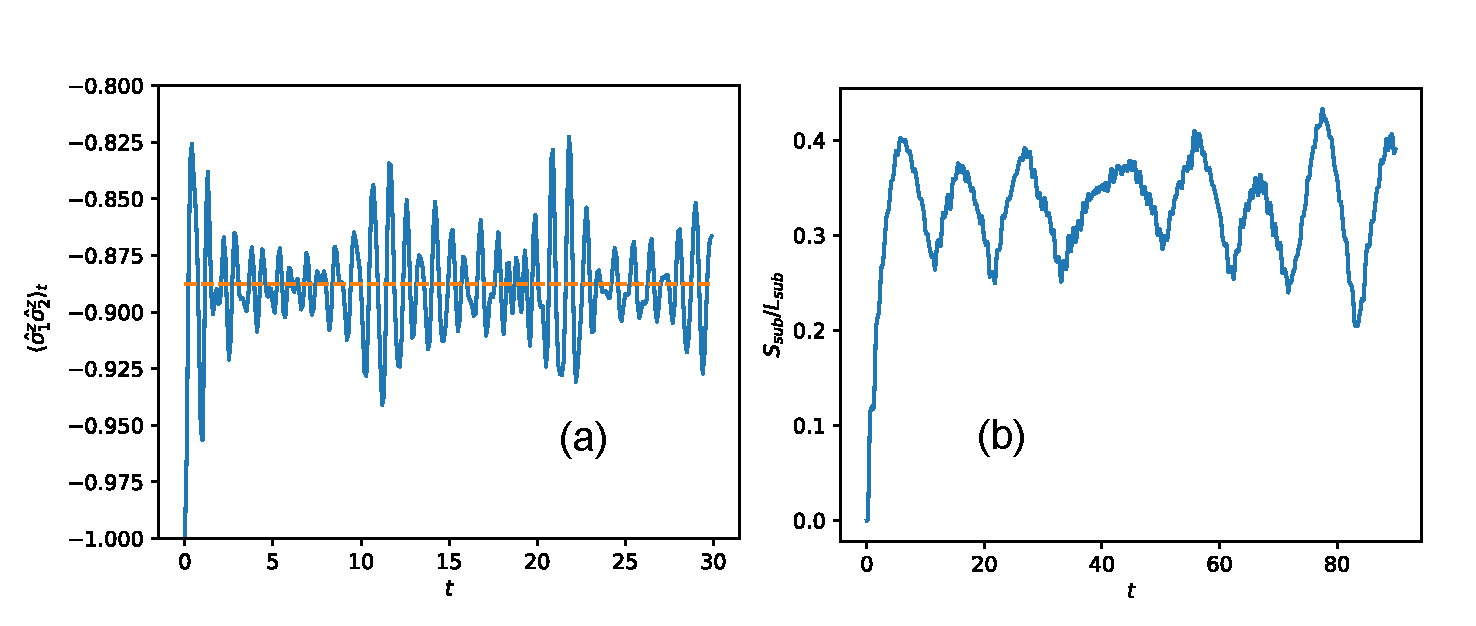
\includegraphics[width=1.0\textwidth]{./scar/scar5.pdf}
\bicaption{图(a)代表初态为$|Z_2\rangle$的动力学演化。图(b)为第一个格点的纠缠熵随时间的变化。我们选取此时链长为$L=16$。橘黄色虚线代表有限尺寸修正后下的热力学吉布斯正则系综平均。我们选取$L=16, J=2.3, h=1.1$。}{Fig (a) for dynamics of local operator $\hat{L}=\hat{\sigma}_1^z\hat{\sigma}_2^z$ starting from$|Z_2\rangle$. Orange dashed line for Gibbs canonical ensemble average of after finite size scaling. Fig (b) for entanglement entropy dynamics of spin degree on first site. We choose $L=16, J=2.3, h=1.1$ for simulation.}
\label{weak}
\end{figure}
%***********************************

最后在中间区域$h\sim 1, J \sim 1$附近,我们从$|Z_2\rangle$出发的动力学结果表明此时热化仍然是很慢的,其行为类似于之前观测到的弱热化行为,与此时选取初态为$|Y-\rangle = |Y-\rangle_0 \otimes|Y-\rangle_1\otimes |Y-\rangle_2 \otimes... $的热化动力学有很大不同,局域算符与单自旋纠缠熵的动力学中表现出明显强于强热化行为的震荡,单自旋熵的上界为$ln2$,如图~\ref{midweak}~所示。

\section{小结与展望}\label{4sec:sum}
我们选取$|Z_2\rangle$作为初态,进行长时间动力学平均与热力学系综平均的比较,发现这一初态对应的热化相图。首先对于many body scar物理,对应$J:h=1:2$,在此区域我们发现在这个强弱耦合区间内系统时间平均都不等于系综平均。在这一特殊比例附近,对应在PXP模型下加入沿z方向的磁场,这一磁场沿正向和反向都会抑制反差的多体伤痕动力学,但仅在$h_{eff}<0$的时候会彻底破坏。在$J\gg h/2$的弱热化区域下,我们观察到了靠近基态带来的弱热化动力学,并给出简单的准粒子激发解释。最后在中间区域,我们也观测到了弱热化的迹象,并与此时强热化的动力学做了对比,其中单自旋熵的震荡行为揭示了这一点。

尽管我们选取了初态为$|Z_2\rangle$,但是选取比如$|Z_0\rangle$作为初态的动力学也是值得继续研究的,讨论这些初态的异同可以帮助我们得到关于相图更加全面和系统的认识,这是在未来理解热化现象研究中值得进一步探索的。




%***********************************
\begin{figure}[h]
\centering
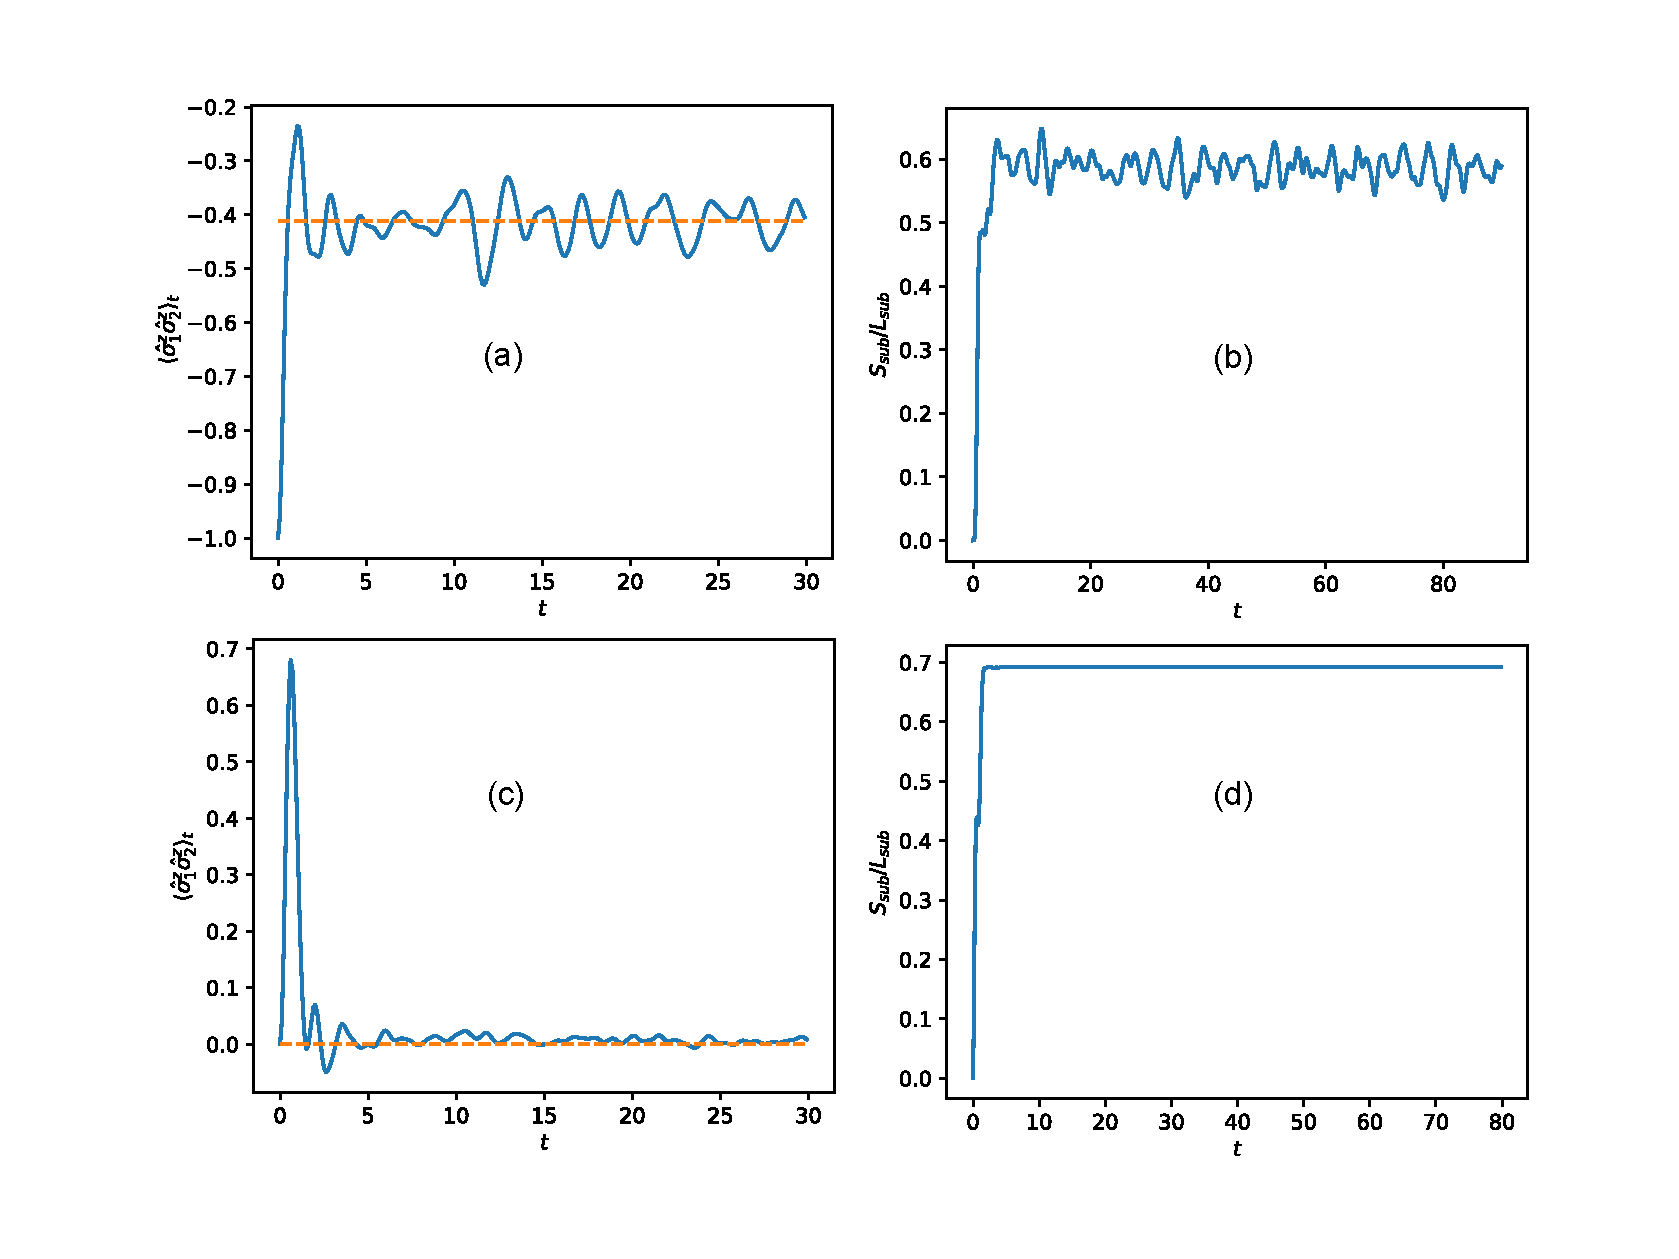
\includegraphics[width=1.0\textwidth]{./scar/scar6.pdf}
\bicaption{图(a,b)为$J=0.9,h=0.8,L=16$下初态为$|Z_2\rangle$的局域算符$\hat{L}=\hat{\sigma}_1^z\hat{\sigma}_2^z$动力学演化(a)与第一格点纠缠熵的动力学演化(b)。图(c,d)为同参数下初态为$|Y-\rangle$的局域算符$\hat{L}=\hat{\sigma}_1^z\hat{\sigma}_2^z$动力学演化(a)与第一格点纠缠熵的动力学演化(b)。橘黄色虚线代表有限尺寸修正后的热力学吉布斯正则系综平均。}{ Fig (a, b) for dynamics of local operator $\hat{L}=\hat{\sigma}_1^z\hat{\sigma}_2^z$(a) and entanglement entropy of spin degree on first site(b) starting from $|Z_2\rangle$. Fig (c,d ) for dynamics of local operator $\hat{L}=\hat{\sigma}_1^z\hat{\sigma}_2^z$(c) and entanglement entropy of spin degree on first site(d) starting from $|Y-\rangle$. We choose $L=16, J=0.9, h=0.8$ for simulation. Orange dashed lines in Fig (a, c) for Gibbs canonical ensemble average after finite size scaling. }
\label{midweak}
\end{figure}
%***********************************








\chapter{总结与展望}\label{chap:summaryandoutlook}

\section{总结}
随着冷原子实验技术的进步,越来越多不同于传统固体物理的实验体系可以在实验中实现。基于这些新的实验体系,有丰富的理论规律以待去探索。本文便沿着样这样一条思路。

我们先从少体杂质体系出发,探究了自旋交换相互作用体系局域自旋杂质与两个巡游费米子相互作用的能谱结构。其中铁磁耦合与反铁磁耦合带来基态特殊的屏蔽效应。而对于激发态upper branch,我们研究了这些特殊的激发态自旋与空间部分行为,利用无限大耦合附近下的简并微扰论研究其能级劈裂行为。其中最为特殊的铁磁upper branch由于对称性的保护与lower branch之间耦合为零,并且具有良好的自旋电荷分离的行为。通过系统地分析少体体系的能谱,我们期望在少体中发现的特殊关联规律可以在多体极限下有所保留。

接着我们从少体研究转到多体物理。我们考虑一个运动杂质与背景费米海相互作用体系的基态转变。采用统一截止到两对电子空穴激发的变分波函数V-2ph,我们理清了在不同维度下的极化子到分子转变的存在性。在三维和二维下,存在这一一阶转变。在二维下我们还用高斯态变分方法进一步证实了这一结论。在一维下我们用V-2ph与贝特假设一起验证了一维下不存在这一转变。 在我们统一波函数的框架下这一转变对应1+N体系基态总动量从零动量到费米动量的转移。我们最终得到结论这一转变来自于粒子空穴激发于泡利不相容原理的共同作用。通过揭示分子态变分波函数为动量为$k_F$的极化子波函数的强耦合渐近描述,我们发现了分子态这一巨大的简并。这一简并在实际体系有限温度有限密度的情况下,会在极化子与分子共存区间增大分子态的占据数。考虑局域密度近似我们计算了实际体系下平均准粒子留数、contact以及极化子能量,并于实验做了细致比较。V-2ph考虑高阶的粒子空穴激发导致准粒子留数降低,因此在弱耦合区间与共振区间与实验符合相比V-1ph较好。

通过上述少体到多体探索,我们研究了杂质体系中相互作用诱导的关联以及维度变化导致的新奇物理。在考虑以上能谱的静态信息之后,我们转向考虑能谱的动力学特征。我们系统地考虑了带有纵场的横场伊辛模型,通过从不同的初态出发,探索了整个参数区间的热化相图。得到不同相区的分界,并对不同相区做了分析。以期对热化动力学有更加系统全面的认知。

\section{展望}
\subsection{少体物理}
在我们计算完成1+2三体体系之后,一个自然的问题是如果继续放入一个巡游费米子变成四体体系会怎样?由于此时系统的自由度距离数值计算的上限自由度还较远,这个问题可以此框架下直接处理。甚至更进一步,我们继续增加巡游费米子,一个自然的问题就是局域杂质束缚巡游费米子的数目是否存在上界?如果存在上界这个上界是由自选所决定吗?以及在反铁磁耦合下增加巡游费米子到近藤物理区间,这一束缚态与近藤单态之间有何联系?这些问题都是值得考虑的。

再者冷原子物理中除了自旋交换相互作用以外,研究较为广泛的还有偶极相互作用,如果在三体体系中将相互作用变成偶极相互作用,那体系的能谱将会有怎样的结构,是否有新的特殊关联出现?这也是值得继续探索的。

\subsection{极化子}
基于我们扩展到有限动量V-2ph,在二维情况下,我们的计算能力以及迭代算法允许我们考虑更高阶的激发V-3ph。在V-3ph中,除了两原子分子态的特殊关联之外,三原子分子态、四原子分子态关联也可以考虑进来。当考虑三、四原子分子态的时候,我们需要进一步放松杂质原子与背景费米子质量比约束。因为这涉及到真空中三体、四体分子态的形成。基于上述简单图像,我们在此方向上有了初步的探索,分别是一个少体体系与多体体系。在少体体系的探索中,我们考虑一个杂质最多可以与多少个背景费米子在真空下形成束缚态。在幺正极限下,我们发现三体分子态出现的临界质量为3.38,四体分子态出新的临界质量为5.14。这两类多体分子态的内禀角动量均为零。但是在动量空间中的粒子空穴关联却展示出很大不同。这种不同可以用原子-分子配对来理解。在多体体系,我们考虑V-3ph变分波函数,研究改变质量比下极化子到三体分子以及四体分子的转变。在超过相应的临界质量比之后,不同极化子到两体分子的一阶转变,极化子到三体分子以及四体分子的转变是一个连续渡越。多体背景下三体与四体关联导致了动量分布晶格化的特征。为进一步探索超越超流配对图像的费米-费米混合气体打开突破口。以上两者扩展都有希望在目前的冷原子实验技术下直接探测验证。




%---------------------------------------------------------------------------%
% main content
%-
%-> Appendix
%-
\cleardoublepage%
\appendix% initialize the environment
\chapter{中国科学院大学学位论文撰写要求}

学位论文是研究生科研工作成果的集中体现,是评判学位申请者学术水平、授予其学位的主要依据,是科研领域重要的文献资料。根据《科学技术报告、学位论文和学术论文的编写格式》(GB/T 7713-1987)、《学位论文编写规则》(GB/T 7713.1-2006)和《文后参考文献著录规则》(GB7714—87)等国家有关标准,结合中国科学院大学(以下简称“国科大”)的实际情况,特制订本规定。

\section{论文无附录者无需附录部分}

\section{测试公式编号 \texorpdfstring{$\Lambda,\lambda,\theta,\bar{\Lambda},\sqrt{S_{NN}}$}{$\textLambda,\textlambda,\texttheta,\bar{\textLambda},\sqrt{S_{NN}}$}} \label{sec:testmath}

\begin{equation} \label{eq:appedns}
    \adddotsbeforeeqnnum%
    \begin{cases}
        \frac{\partial \rho}{\partial t} + \nabla\cdot(\rho\Vector{V}) = 0\\
        \frac{\partial (\rho\Vector{V})}{\partial t} + \nabla\cdot(\rho\Vector{V}\Vector{V}) = \nabla\cdot\Tensor{\sigma}\\
        \frac{\partial (\rho E)}{\partial t} + \nabla\cdot(\rho E\Vector{V}) = \nabla\cdot(k\nabla T) + \nabla\cdot(\Tensor{\sigma}\cdot\Vector{V})
    \end{cases}
\end{equation}
\begin{equation}
    \adddotsbeforeeqnnum%
    \frac{\partial }{\partial t}\int\limits_{\Omega} u \, \mathrm{d}\Omega + \int\limits_{S} \unitVector{n}\cdot(u\Vector{V}) \, \mathrm{d}S = \dot{\phi}
\end{equation}
\[
    \begin{split}
        \mathcal{L} \{f\}(s) &= \int _{0^{-}}^{\infty} f(t) e^{-st} \, \mathrm{d}t, \ 
        \mathscr{L} \{f\}(s) = \int _{0^{-}}^{\infty} f(t) e^{-st} \, \mathrm{d}t\\
        \mathcal{F} {\bigl (} f(x+x_{0}) {\bigr )} &= \mathcal{F} {\bigl (} f(x) {\bigr )} e^{2\pi i\xi x_{0}}, \ 
        \mathscr{F} {\bigl (} f(x+x_{0}) {\bigr )} = \mathscr{F} {\bigl (} f(x) {\bigr )} e^{2\pi i\xi x_{0}}
    \end{split}
\]

mathtext: $A,F,L,2,3,5,\sigma$, mathnormal: $A,F,L,2,3,5,\sigma$, mathrm: $\mathrm{A,F,L,2,3,5,\sigma}$.

mathbf: $\mathbf{A,F,L,2,3,5,\sigma}$, mathit: $\mathit{A,F,L,2,3,5,\sigma}$, mathsf: $\mathsf{A,F,L,2,3,5,\sigma}$.

mathtt: $\mathtt{A,F,L,2,3,5,\sigma}$, mathfrak: $\mathfrak{A,F,L,2,3,5,\sigma}$, mathbb: $\mathbb{A,F,L,2,3,5,\sigma}$.

mathcal: $\mathcal{A,F,L,2,3,5,\sigma}$, mathscr: $\mathscr{A,F,L,2,3,5,\sigma}$, boldsymbol: $\boldsymbol{A,F,L,2,3,5,\sigma}$.

vector: $\Vector{\sigma, T, a, F, n}$, unitvector: $\unitVector{\sigma, T, a, F, n}$

matrix: $\Matrix{\sigma, T, a, F, n}$, unitmatrix: $\unitMatrix{\sigma, T, a, F, n}$

tensor: $\Tensor{\sigma, T, a, F, n}$, unittensor: $\unitTensor{\sigma, T, a, F, n}$ 


% appendix content
%-
%-> Backmatter: bibliography, glossary, index
%-
\backmatter% initialize the environment
\intotoc*{\cleardoublepage}{\bibname}% add link to toc
\artxifstreq{\artxbib}{bibtex}{% enable bibtex
    \bibliography{Biblio/ref}% bibliography
}{%
    \printbibliography% bibliography
}
%---------------------------------------------------------------------------%
%->> Backmatter
%---------------------------------------------------------------------------%
\chapter[致谢]{致\quad 谢}\chaptermark{致\quad 谢}% syntax: \chapter[目录]{标题}\chaptermark{页眉}
%\thispagestyle{noheaderstyle}% 如果需要移除当前页的页眉
%\pagestyle{noheaderstyle}% 如果需要移除整章的页眉

感谢...

\chapter{作者简历及攻读学位期间发表的学术论文与研究成果}


\section*{作者简历:}

彭程,山东省潍坊市人,中国科学院物理研究所博士研究生。

\section*{已发表(或正式接受)的学术论文:}

{
\setlist[enumerate]{}% restore default behavior

\begin{enumerate}[nosep]
    \item {\bfseries\sffamily Cheng Peng}, Xiaoling Cui, Few-body solutions under spin-exchange interaction: Magnetic bound state and the Kondo screening effect, Phys. Rev. A. 102, 033312(2020)
    
    \item {\bfseries\sffamily Peng, Cheng*}, Ruijin Liu*, Wei Zhang , Xiaoling Cui, Nature of the polaron-molecule transition in Fermi polarons, Phys. Rev. A. 103, 063312(2021)

    \item Yinfeng Ma, {\bfseries\sffamily Cheng Peng}, Xiaoling Cui, Borromean Droplet in Three-Component Ultracold Bose Gases, Phys. Rev. Lett. 127, 043002(2021)

    \item Ruijin Liu, {\bfseries\sffamily Cheng Peng}, Xiaoling Cui, Universal tetramer and pentamer in two-dimensional fermionic mixtures, arXiv:2202.01437

    \item Ruijin Liu, {\bfseries\sffamily Cheng Peng}, Xiaoling Cui, Emergence of Crystalline Few-body Correlations in Mass-imbalanced Fermi Polarons, arXiv:2202.03623

\end{enumerate}
}


\section*{参加的研究项目及获奖情况:}
...

\cleardoublepage[plain]% 让文档总是结束于偶数页,可根据需要设定页眉页脚样式,如 [noheaderstyle]
%---------------------------------------------------------------------------%
% other information
\end{document}
%---------------------------------------------------------------------------%
